\documentclass[11pt]{article}
\usepackage{fullpage}

\usepackage{amsthm,amsmath,amssymb}

\usepackage[bookmarks=true,hypertexnames=false,pagebackref]{hyperref}
\hypersetup{colorlinks=true, citecolor=blue, linkcolor=red,
  urlcolor=blue}
\usepackage{amsthm}
\usepackage[lining,semibold,type1]{libertine} % a bit lighter than Times--no osf in math
\usepackage[T1]{fontenc} % best for Western European languages
\usepackage{textcomp} % required to get special symbols
\usepackage[varqu,varl]{inconsolata}% a typewriter font must be defined
\usepackage[libertine,vvarbb]{newtxmath}
\usepackage[scr=rsfso,cal=cm]{mathalfa}
\usepackage{bm}
\usepackage{cleveref}
\usepackage{graphicx}
\usepackage{todonotes}
\usepackage{enumerate}
\usepackage{thmtools}

% \usepackage{natbib}

\newtheorem{theorem}{Theorem}
\newtheorem{lemma}[theorem]{Lemma}
%\newtheorem{problem}[theorem]{Problem}
\newtheorem{corollary}[theorem]{Corollary}
\newtheorem{definition}[theorem]{Definition}
\newtheorem{definitions}[theorem]{Definitions}
\newtheorem{conjecture}[theorem]{Conjecture}
\newtheorem{claim}[theorem]{Claim}
\newtheorem{fact}[theorem]{Fact}
\newtheorem{block}[theorem]{}
\newtheorem*{myclaim}{Claim}
\newtheorem*{remark}{Remark}
\newtheorem{proposition}[theorem]{Proposition}
\newtheorem{condition}{Condition}
\newtheorem{problem}{Problem}
\newtheorem{property}{Property}

\crefname{condition}{Condition}{Conditions}
\crefname{proposition}{Proposition}{Propositions}
\crefname{lemma}{Lemma}{Lemmas}
\crefname{theorem}{Theorem}{Theorems}

% \DeclareMathAlphabet{\mathcal}{OMS}{cmsy}{m}{n}
% \DeclareSymbolFont{largesymbols}{OMX}{cmex}{m}{n} % This command seems not compatible with the package {newtxmath}

\newcommand{\norm}[1]{\left\Vert#1\right\Vert}
\newcommand{\abs}[1]{\left\vert#1\right\vert}
\newcommand{\set}[1]{\left\{#1\right\}}
\newcommand{\tuple}[1]{\left(#1\right)} \newcommand{\eps}{\varepsilon}
\newcommand{\inner}[2]{\langle #1,#2\rangle} \newcommand{\tp}{\tuple}
\renewcommand{\mid}{\;\middle\vert\;} \newcommand{\cmid}{\,:\,}
\newcommand{\numP}{\#\mathbf{P}} \renewcommand{\P}{\mathbf{P}}
\newcommand{\defeq}{\triangleq} \renewcommand{\d}{\,\-d}
\newcommand{\ol}{\overline}

\newcommand{\id}[1]{\mathbb{1}\left[#1\right]}

\usepackage[ruled,linesnumbered,vlined]{algorithm2e}
%\renewcommand{\thealgorithm}{} %% disable the algorithm counter
\usepackage{algpseudocode}
\SetKwRepeat{Do}{do}{while}

\def\*#1{\mathbf{#1}} \def\+#1{\mathcal{#1}} \def\-#1{\mathrm{#1}} \def\^#1{\mathbb{#1}} \def\$#1{\mathtt{#1}}
\newcommand{\bb}{\mathbb}

\def\!#1{\mathtt{#1}}
\def\@#1{\mathscr{#1}}

\def\EG{\emph{e.g.}}
\def\IE{\emph{i.e.}}

% Zhidan's macros
\def\bad{\!{bad}}
\def\cp{\!{cp}}
\def\good{\!{good}}
\def\poly{\mathrm{poly}}

\def\symbolwidth{\phantom{{}={}}}

\newcommand{\wt}[1]{\widetilde{#1}}
\newcommand{\wh}[1]{\widehat{#1}}
\newcommand{\BuildTime}{\poly\left(\Delta^{\Delta\ell}\right)}
\newcommand{\Couple}{\!{Couple}}
\newcommand{\Ham}{\!{Ham}}
\newcommand{\Holant}{\mathrm{Holant}}
\newcommand{\Par}{\!{Par}}
\newcommand{\Pick}{\!{Pick}}
\newcommand{\RunningTimeExponent}{\poly\left((1 + r^2)^{\Delta}\right)}

\newcommand{\zero}{\boldsymbol{0}}
\newcommand{\vecf}{\boldsymbol{f}}
\newcommand{\seqS}{\boldsymbol{s}}

\usepackage{xifthen}
\usepackage{thm-restate}

\renewcommand{\Pr}[2][]{ \ifthenelse{\isempty{#1}}
  {\mathbf{Pr}\left[#2\right]} {\mathbf{Pr}_{#1}\left[#2\right]} }
\newcommand{\E}[2][]{ \ifthenelse{\isempty{#1}}
  {\mathbf{E}\left[#2\right]}
  {\mathop{\mathbf{E}}_{#1}\left[#2\right]} }
\newcommand{\Var}[2][]{ \ifthenelse{\isempty{#1}}
  {\mathbf{Var}\left[#2\right]}
  {\mathop{\mathbf{Var}}_{#1}\left[#2\right]} }


\newcommand{\zdtodo}[1]{\todo[color = blue!40, size = \tiny]{\textbf{zhidan:} #1}}
\newcommand{\qtodo}[1]{\todo[color = purple!40, size = \tiny]{\textbf{guoliang:} #1}}
\newcommand{\ctodo}[1]{\todo[color = lime!40, size=tiny]{\textbf{Chihao:} #1}}

\newcommand{\qgl}[1]{{\color{purple}{#1}}}
\newcommand{\hktodo}[1]{{\color{blue}{#1}}}

\newcommand{\zd}[1]{{\color{green} #1}}
\newcommand{\zdnew}[1]{{\color{cyan} #1}}
%%% article specific macros %%%

\title{Deterministic Counting}
\author{}
%\address{Shanghai Jiao Tong University}

%\date{Last modified on Oct 28, 2020}
\date{\today}
\begin{document}

\maketitle

\section{Introduction}

Holant problems, namely the read-twice counting CSP, are a family of expressive framework for counting problems. An instance of (binary) Holant problem is a tuple $\Phi=(G=(V,E),\set{f_v}_{v\in V})$ where each $f_v:\set{0,1}^{E(v)}\to \bb C$ is a constraint function with domain $E(v)$, the set of edges incident to $v$. The problem is to compute the \emph{Holant}, or the \emph{partition function} defined as \ctodo{use $E(v)$ or $E_v$?}
\[
    \-{Holant}(\Phi) = \sum_{\sigma\in\set{0,1}^E} \prod_{v\in V}f_v(\sigma|_{E(v)}),
\]
where $\sigma|_{E(v)}$ is the restriction of $\sigma$ on $E(v)$. The framework encodes a broad family of counting problems including counting matchings ($f_v(\tau) = \id{\abs{\tau}\le 1}$), perfect matchings ($f_v(\tau) = \id{\abs{\tau}= 1}$), counting edge covers ($f_v(\tau) = \id{\abs{\tau}\ge 1}$) etc. 

Despite the success in classifying the exact counting complexity~\cite{}, it has been a long-term yet incomplete task to understand their approximability. Even for those \emph{symmetric} constraint functions, namely those $f_v(\tau)$ whose value only depends on the Hamming weights of $\tau$, the complete picture is far from clear. 

One notable benchmark problem for algorithmic techniques is the problem of counting $b$-matchings, which asks for the number of $\set{0,1}$-assignments to edges such each vertex is adjacent to \emph{at most} $b$ edges with value $1$. It can be phrased in the Holant framework where each $f_v(\tau)=\id{\abs{\tau}\le b}$. Clearly, when $b=1$, it is the counting matching problem, which has been a central problem in approximate counting. However, when $b$ becomes larger, many good properties of matchings break down, posing new challenges in algorithm design. The problem was perhaps first studied in the work of ~\cite{}, in which the rapid mixing of a particular Markov chain whose stationary distribution is the uniform distribution over all $b$-matchings was established for $b\le 7$ using the method of canonical paths. Recently, using a simple and neat coupling argument, among many other things, the \emph{spectral independence} property for the uniform distribution of $b$-matching was establish in ~\cite{}, which implies the rapid mixing of Glauber dynamics for sampling $b$-mathcings. As a result, one obtains fully polynomial-time randomized approximation scheme (FPRAS) for counting $b$-matchings for any $b$.

In this work, we focus on \emph{deterministic} approximate counting algorithms. There are a few popular techniques for designing deterministic algorithms, including the method of correlation decay and polynomial interpolation, which result in fully polynomial-time approximation schemes (FPTAS) for counting problems. Both the methods of correlation decay and polynomial interpolation are successful for counting matchings and many other Holant problems. However, for $b$ larger than $1$, the problem of $b$-matching resists both methods: the problem lacks a concise and lossless recursion for computing marginals necessary to apply the correlation decay technique, and it is challenging to determine the location of zeros for the partition function in order to use the polynomial interpolation method. 

We design FPTAS for $b$-matching and more generally Holant problems with log-concave signature by developing the method of linear programming, invented by Moitra in \cite{}, and was previously only applied to counting problems on hypergraphs. 

\subsection{Main results}

\paragraph{\ensuremath{b}-matchings}

Given a graph $G = (V, E)$, let $E_v \defeq \set{e \in E \cmid \mbox{$e$ is incident to $v$}}$ be the collection of all edges incident to $v$ for each $v \in V$. For a positive integer $b \ge 1$, we say that $S \subseteq E$ is a \emph{$b$-matching of $G$} if $\abs{S \cap E_v} \le b$ for every $v \in V$. Let $\Omega = \Omega_{G, b}$ be the set of all $b$-matchings and $\mu = \mu_{G, b}$ be the uniform distribution over $\Omega$. 
% \qgl{Moreover, we remark here that the definitions above can be safely extended to graphs with dangling edges.}\qtodo{In introduction, it is not necessary to introduce the notion of dangling edges.}

\zdtodo{State SOTA of $b$-matchings here, and following is our main result on it.}

\begin{theorem} \label{thm:counting-b-matchings}
    Given positive integers $\Delta > 0$, there is an FPTAS for counting the number of $b$-matchings for any graph with maximum degree $\Delta$ and every positive integer $b > 0$.
\end{theorem}
\zdtodo{suggest this version: the running time is seemingly slow.}

\begin{theorem} \label{thm:counting-b-matchings}
    There exists a deterministic algorithm that given any graph $G = (V, E)$ with maximum degree $\Delta$, any positive integer $b \ge 1$ and any $\varepsilon \in (0, 1)$, it outputs a number $\wh{Z}$ such that
    \begin{align*}
        (1 - \varepsilon)\abs{\Omega_{G, b}} \le \wh{Z} \le (1 + \varepsilon) \abs{\Omega_{G, b}}
    \end{align*}
    in time $(\abs{E} \cdot \varepsilon^{-1})^{\poly(\Delta^b)}$.
\end{theorem}

\paragraph{Holant problems with log-concave signatures}

Beyond counting the number of $b$-matchings, we also consider a family of Holant problems with binary symmetric log-concave signatures. Given a function $f$ of arity $d > 0$, we say that $f$ is \emph{binary symmetric} if $f : \set{0, 1}^d \to \mathbb R_{\ge 0}$ and its value only depends on the hamming weight of the input. By symmetry, it is safe to identity $f$ as $f = [f(0), f(1), \ldots, f(d)]$.

For a family of binary symmetric functions $\+F$, the Holant problem, denoted by $\Holant(\+F)$, is a family of counting problems defined on graphs by assigning a signature in $\+F$ to each vertex in the graph. Specifically, an instance of $\Holant(\+F)$ can be specified by $ \Phi = \left(G = (V, E), \vecf = \set{f_v}_{v \in V}\right)$ where for each $v \in V$, $f_v \in \+F$ is called the \emph{signature at $v$}. \qtodo{We should introduce the external field here?}
The counting problem is to (approximately) compute the partition function $Z= Z_\Phi$ defined as follows:
$$
   Z\defeq \sum_{\sigma\in \set{0,1}^{E}} \prod_{v \in V} f_v\left(\abs{\sigma \vert_{E_v}}\right),
$$ where $\sigma \vert_{E_v}$ is the restriction of $\sigma$ on the edges $E_v$.
%\qtodo{Use $\sigma \vert_{E_v}$ or $\sigma_{E_v}$?}
% Then the corresponding Gibbs distribution $\mu = \mu_\Phi$ can be defined as
% % \begin{align*}
% %     \mu(\sigma) = \mu_\Phi(\sigma) \defeq \frac{1}{Z} \prod_{v \in V} f_v\left(\abs{\sigma_{E_v}}\right), \quad \forall \sigma \in \set{0,1}^{E},
% % \end{align*} 
% \begin{align*}
%     \mu(S) \defeq \frac{1}{Z} \prod_{v \in V} f_v(\abs{S \cap E_v}), \quad \forall S \subseteq E,
% \end{align*} 
% where $Z= Z_\Phi$ is the partition function defined as $ Z  \defeq \sum_{S \subseteq E} \prod_{v \in V} f_v(\abs{S \cap E_v})$. 
Furthermore, it is natural to induce the probability distribution $\mu=\mu_\Phi$ over $\Omega = \Omega_\Phi=\set{0,1}^{E}$ where 
\begin{equation}\label{def-holant-mu}
\begin{aligned}
\forall \sigma\in \Omega, \quad \mu(\sigma)=\frac{1}{Z}  \prod_{v \in V} f_v\left(\abs{\sigma \vert_{E_v}}\right)
\end{aligned}
\end{equation}
% \begin{align*}
%    \mu(\sigma)\triangleq \frac{1}{Z} \prod_{v \in V} f_v\left(\abs{\sigma_{E_v}}\right).
% \end{align*}
% \begin{align*}
%     Z  \defeq \sum_{S \subseteq E} \prod_{v \in V} f_v(\abs{S \cap E_v}).
% \end{align*}
% $$
% \begin{gathered}
% 	\mu(S) = \mu_\Phi(S) \defeq \frac{1}{Z} \prod_{v \in V} f_v(\abs{S \cap E_v}), \quad \forall S \subseteq E, \\
% 	Z = Z_\Phi \defeq \sum_{S \subseteq E} \prod_{v \in V} f_v(\abs{S \cap E_v}).
% \end{gathered}
% $$
\qgl{When $f_v(k) = \id{k \le b}$, it can be shown that the Holant problem becomes an instance of $b$-matchings by regarding any subset of edges $S\subseteq E$ as the binary vector.} \qtodo{maybe add more famous problem here to show the expressibility of the holant.}

%Note that, for a Holant instance $(G = (V, E), \set{f_v}_{v \in V})$, 
In this paper, we focus on a family of Holant problems with signatures being log-concave. A binary symmetric signature $f = [f(0), f(1), \ldots, f(d)]$ of arity $d$ is \emph{log-concave} if and only if it satisfies: (1) $f(k)^2 \ge f(k - 1) f(k + 1)$ for every $1 \le k \le d - 1$; (2) If $f(k_1) > 0$ and $f(k_2) > 0$ for some $0 \le k_1 \le k_2 \le d$, then for every $k_1 \le j \le k_2$, $f(j) > 0$. We say that $\Phi = \left(G = (V, E), \vecf = \set{f_v}_{v \in V}\right)$ is log-concave if all its signatures are log-concave. 
We always assume \emph{w.l.o.g.} that $f_v(d)=0$ for each $v\in V$ and $d> \Delta$, where $\Delta$ is the maximum degree of $G$.
\qgl{state that the log-concave signature is powerful enough to express many counting problems.}

We consider a family of Holant instances satisfying the following conditions.
\begin{condition} \label{cond:Holant-condition}
    Consider the Holant instance $\Phi=(G= (V, E),\vecf)$ satisfying that $\vecf = \set{f_v}_{v \in V}$ is a family of binary symmetric log-concave signatures and $f_v(0) > 0$ for every $v \in V$.

\end{condition}

% \begin{condition} \label{cond:Holant-condition}
%     Let $\Delta$ be a positive integer. Consider the Holant instance $\Phi = (G=(V,E), \vecf)$ satisfying 
%     \begin{itemize}
%         \item $\Delta(G)\leq \Delta$;
%         \item $\vecf = \set{f_v}_{v \in V}$ is a family of binary symmetric log-concave signatures and $f_v(0)>0$ for each $v\in V$.
%     \end{itemize}
% \end{condition}

\zdtodo{State SOTA of Holant problems with log-concave signatures here, and following is our main result on it.}

% \begin{theorem} \label{thm:counting-Holant}
%     Given a positive integer $\Delta > 0$ and a real number $r > 0$, there is an FPTAS for the partition function of every Holant instance $\Phi = \left(G = (V, E), \vecf = \set{f_v}_{v \in V}\right)$ satisfying~\Cref{cond:Holant-condition} with the maximum degree of $G$ at most $\Delta$ and $f_v(1) \le r f_v(0)$ for each $v \in V$.
% \end{theorem}
% \zdtodo{suggest this version: the running time is seemingly slow.}

\begin{theorem} \label{thm:counting-Holant}
    There is a deterministic algorithm such that given as input any $\varepsilon>0$ and any instance $\Phi = \left(G = (V, E), \vecf = \set{f_v}_{v \in V}\right)$ satisfying~\Cref{cond:Holant-condition}, it outputs a number $\wh{Z}$ such that
    $$
        (1 - \varepsilon) Z_\Phi \le \wh{Z} \le (1 + \varepsilon) Z_{\Phi}
    $$
    \zdnew{within time $(\abs{E} \cdot \varepsilon^{-1})^{\RunningTimeExponent}$. Here $\Delta$ is the maximum degree of $G$ and $r = \max_{v} \frac{f_v(1)}{f_v(0)}.$}
    % \qgl{within time $\poly\left(\left(\abs{E} \cdot \varepsilon^{-1}\right)^{C_{\ref{thm:counting-Holant}}}\right)$ where coefficients of the polynomial and $C_{\ref{thm:counting-Holant}}$ depend only on $\Delta$ and $r$. Here $\Delta$ is the maximum degree of $G$ and $r=\max_v \frac{f_v(1)}{f_v(0)}$.} 
    \qtodo{continue here later}
\end{theorem}

\subsection{Technique overview}


\section{Preliminaries}

\subsection{Notations}

For a natural number $n \in \mathbb N$, we use $[n]$ to denote the set $\set{1, 2, \ldots, n}$.
We use $\log(\cdot)$ to denote the logarithm with the natural base.
For an event $\+E$, we use $\id{\+E}$ to denote the indicator of it. 
We will use boldface type, e.g., $\boldsymbol{S},\boldsymbol{c}$, for vectors.
Specifically, we use $\boldsymbol{0}$ and $\boldsymbol{1}$ to denote the all-zero vector and the all-one vector, respectively.
For any sequence $\seqS = (s_1, \ldots, s_\ell)$ and any element $t$, let $\seqS \circ t$ denote $(s_1, \ldots, s_\ell,t)$, the concatenation of $\seqS$ and $t$.
With a slight abuse of notation, we will occasionally use the sequence $\seqS= (s_1, \ldots, s_\ell)$ to denote the set $\{s_1, \ldots, s_\ell\}$ when it is clear from the context.
% Let $\seqS = \set{s_1, \ldots, s_\ell}$ be an ordered sequence of length $\ell$ and $\alpha$ be an element, we use $\seqS \circ \alpha$ to denote the concatenation of $\seqS$ and $\alpha$ defined as $\seqS \circ e \defeq \set{s_1, \ldots, s_\ell, s_{\ell + 1} = \alpha}$. 
Moreover, we use the notation $\varnothing$ to denote an empty sequence.

We consider the graphs with ``half-edges'' in this paper.
Formally, given a set of nodes $V$, an \emph{normal} edge on $V$ is a pair of different nodes $\{u,v\}$ where $u,v\in V$,
and a half-edge on $v$ is a singleton tuple $\{u\}$ where $u \in V$.
A graph with half-edges is a pair $(V,E_1\cup E_2)$ where $V$ is a set of nodes, $E_1$ is a set of normal edges,
and $E_2$ is a set of half-edges. 
\qgl{To distinguish the graph with no half-edges, we will consistently refer to the graph with half-edges as $G=\left(V,E=E_1\cup E_2\right)$. One can verify that the notations $\mu_\Phi$, $Z_\Phi$, e.t.c., can be generalized to the instances where the graph has half edges.}
% \hktodo{
% For convenience, we allow the ``half-edges'' in the graph $G=(V,E)$ we considered. These half-edges refer to the edges in the graph which have only one endpoint. Then we write $E = E_1 \cup E_2$ where $E_1$ is the set of all normal edges and $E_2$ collects all half-edges in $G$. }
Given a graph $G$, we always use $V(G)$ to denote the vertex set of $G$, $E(G)$ to denote the edge set, $E_1(G) \subseteq E(G)$ to denote the collection of normal edges, $E_2(G)\subseteq E(G)$ to denote the set of half-edges, and $\Delta(G)$ to denote the maximum degree. 
For every $v \in V$, we use $\deg_G(v)$ to denote the degree of $v$ in $G$, \IE, the number of edges incident to $v$.
% We also let $\Delta(G)$ be the maximum degree of $G$. 
If $G$ is clear from the context, we may omit $G$ from these notations.
% When the context is clear, we omit explicitly indicating the graph $G$. 
For convenience, we suppose that an arbitrary order is assumed over all the edges in $E_1$.
% For convenience, we fix an arbitrary order to the edges.

% Given a rooted tree $T = (V(T), E(T))$, we use $\rho = \rho(T)$ to denote its root. For every vertex $v \in V(T)$, we use $\Par(v)$ to denote the parent of $v$ and $\+C(v)$ to denote the collection of children of $v$ with convention $\Par(\rho(T)) = \varnothing$.\qtodo{recheck here}

We call $\sigma: E\rightarrow \set{0,1}$ an assignment of $G$.
For any subset $S\subseteq E$ and any assignment $\sigma$, we use $\sigma(S)$ to denote the assignments of $\sigma$ on $S$.
For simplicity, let $\sigma(e)$ denote $\sigma(\{e\})$ for each $e\in E$. For any $S\subseteq E$, we call $\sigma: S\rightarrow \set{0,1}$ a \emph{partial assignment} of $G$ defined on $S$.
For any subset $S \subseteq E$ and any partial assignment $\sigma$ defined on $S$, 
let $\Lambda(\sigma)$ denote $S$.
For any assignment $\sigma$ and any partial assignment $\tau$,
we abuse the notation $\sigma\in \tau$ to denote the event that $\sigma(\Lambda(\tau)) =\tau$.

Given any partial assignment $\sigma$ and any vertex $v \in V$, we use $\Ham(\sigma, E_v)$ to denote $\abs{\sigma(E_v \cap \Lambda(\sigma))}$, i.e., the Hamming weight of $\sigma$ restricted to $E_v \cap \Lambda(\sigma)$.
For two partial assignments $\sigma$ and $\tau$ where $\Lambda(\sigma)\cap \Lambda(\tau) = \emptyset$, we use $\sigma \land \tau : \Lambda(\sigma) \cup \Lambda(\tau) \to \set{0, 1}$ to denote the concatenation of $\sigma$ and $\tau$, \IE, $(\sigma \land \tau)(e)=\sigma(e)$ for each $e\in \Lambda(\sigma)$ and $(\sigma \land \tau)(e)=\tau(e)$ for each $e\in \Lambda(\tau)$. 
{Additionally, for any $S\subseteq E$ and any $\boldsymbol{c} \in \{0,1\}^S$, we use $S \gets \boldsymbol{c}$ to denote the partial assignment $\sigma$ where $\Lambda(\sigma) = S$ and $\sigma(S) = \boldsymbol{c}$.}

Fix an instance $ \Phi = \left(G = (V, E), \vecf = \set{f_v}_{v \in V}\right)$ of the Holant problem.
Recall the distribution $\mu \triangleq \mu_{\Phi}$ defined in \eqref{def-holant-mu}.
We say an assignment $\sigma$ of $G$ is feasible if $\mu(\sigma)>0$. 
We say a partial assignment $\tau$ is \emph{feasible} if there exists a feasible assignment $\sigma\in \tau$.



% We say that $\sigma_{\Lambda}$ is \emph{a feasible partial assignment} if $\set{\sigma\in \set{0,1}^E \ \vert \ \sigma \vert_\Lambda=\sigma_{\Lambda}\land  \mu(\sigma)>0} \neq \emptyset$.

 
% Given a distribution $\mu$ defined among $\set{0,1}^E$, we say an assignment $\sigma: E\rightarrow \set{0,1}$ is feasible if $\mu(\sigma)>0$. For any subset $\Lambda \subseteq E$, we use $\sigma_\Lambda : \Lambda \to \set{0, 1}$ to denote the partial assignment defined on $\Lambda$. 
% We say that $\sigma_{\Lambda}$ is \emph{a feasible partial assignment} if $\set{\sigma\in \set{0,1}^E \ \vert \ \sigma \vert_\Lambda=\sigma_{\Lambda}\land  \mu(\sigma)>0} \neq \emptyset$.
% \hktodo{ Moreover, we abuse the notation $\sigma_{\Lambda}$ to denote the event that $\set{\sigma \vert_\Lambda=\sigma_{\Lambda} \ \vert \ \mu(\sigma)>0}$.}

% With this notation, it is convenient to indicate that the restriction of the assignment $\sigma$ coincides with $\sigma_\Lambda$ by expressing it as $\sigma\in \sigma_{\Lambda}$. 


For any partial assignment $\tau$ and any vertex $v\in V$, we use $E_v^\tau \defeq E_v \setminus \Lambda(\tau)$ to denote the set of unpinned edges incident to $v$ under $\tau$. 
Given any feasible partial assignment $\tau$ and any subset $S \subseteq E \setminus \Lambda(\tau)$, we denote by $\mu_S^\tau$ the marginal probability distribution of $\mu$ projected to $S$ conditional on $\tau$.
Similarly, let $\mu_S$ denote the marginal probability distribution of $\mu$ projected to $S$.
Furthermore, given any partial assignment $\sigma$ where $S\subseteq \Lambda(\sigma)$ and any $e\in E$ where $e\not\in \Lambda(\tau)$, we will use the following simplified notations:
\begin{itemize}
\item Let $\mu_S^\tau(\sigma),\mu_S(\sigma)$ denote $\mu_S^\tau(\sigma(S)),\mu_S(\sigma(S))$, respectively;
\item Let $\mu^\tau(\sigma),\mu(\sigma)$ denote $\mu_{\Lambda(\sigma)\setminus\Lambda(\tau)}^\tau(\sigma),\mu_{\Lambda(\sigma)}(\sigma)$, respectively;
\item Let $\mu_e^\tau(\sigma),\mu_e(\sigma)$ denote $\mu_{\{e\}}^\tau(\sigma),\mu_{\{e\}}(\sigma)$, respectively.
\end{itemize}




\iffalse
\subsection{$b$-matchings and notations}
    Consider a graph $G=(V,E)$ with an integer $b\geq 1$. A $b$-matching of $G$ is a subset of edges $S\subseteq E$ such that for each $v\in V$, we have $\abs{S\cap E_v}\leq b$ where $E_v\triangleq \set{e\in E \mid v\in e}$ is the collection of incident edges of $v$. Let $\Omega=\Omega_{G,b}$ be the set of all $b$-matchings of $G$ and $\mu=\mu_{G,b}$ be the uniform distribution over $\Omega$. 


    For convenience, we use a binary indicator vector $\sigma: E\rightarrow \set{0,1}$ to represent any subset of edge $S\subseteq E$ where $\sigma(e)=1$ if $e\in S$ for each $e\in E$. 
    Moreover, we use $\sigma_S:S\rightarrow \set{0,1}$ to denote the partial assignment defined on $S\subseteq E$ or the partial assignment defined on $S\subseteq E$ induced from $\sigma$, i.e., for any variable $e$ in $S$, we have $\sigma_S(e)=\sigma(e)$. \zdtodo{If necessary: change the notation here. Suggest $\sigma \vert_S$.} \qgl{We sometimes use the notation $v\gets a$ to denote the partial assignment on a single edge.}

    Given any partial assignment $\tau: E'\rightarrow \set{0,1}$ defined on $E'\subseteq E$, we abuse $\tau$ to denote the event that $\set{\sigma_S=\tau \ \vert \ \mbox{$\sigma$ is a $b$-matching}}$. By this notation, we call a partial assignment $\tau$ is feasible if $\tau\neq \emptyset$. (\qgl{and we can use $\tau_1\land \tau_2$ to denote the concatenation of the partial assignments}) Furthermore, given any subset of edges $S\subseteq E\setminus E'$, we use $\mu_S^{\tau}$ to denote the marginal distribution on $S$ conditioned on the event $\tau$. \qgl{In particular $\mu_v=\mu_{\set{v}}$.} \qgl{here, we also define $E^{\tau}_v$ as the unpinned edges in $E_v$.} 
    % We can equivalently view the instance with pinned partial assignment as a instance with no pinning.

    In our later discussion, {we also allow the existence of the \qgl{dangling edges}}. Specifically, we represent the graph by $G=(V,E=E_1\cup E_2)$ where $E_1$ is the set of normal edges and $E_2$ is the set of dangling edges.
    {One can generalize the previous notations and notions in the graph with dangling edges similarly.} 

\subsection{Holant problems with log-concave signatures}

\iffalse
    In this paper, we consider the Holants problem with binary symmetric signatures.
    Given a set of signature $\+F$ where each $f\in \+F$ of arity $d>0$ is a binary symmetric function $f: \set{0,1}^d\rightarrow \^R$ that the value depends only on the hamming weight of the input, the Holant problem, denoted by $\HH(\+F)$ is a family of counting problems defined on the graphs by associating the signature with each vertex in $\+F$. Specifically, an instance of $\HH(\+F)$ can be specified by the tuple $\left(G=(V,E),\set{f_v}_{v\in V}\right)$ where $f_v\in \+F$, and our goal is to compute the following partition function
    \begin{align*}
        \HH(G,\set{f_v}_{v\in V})\triangleq \sum_{\sigma\in \set{0,1}^{E}} \prod_{v\in V} f_v(\sigma_{E_v})
    \end{align*}
    where $f_v(\sigma_{E_v})$ is well-defined by the symmetry of the signature. \qgl{continue here.}
\fi

In this paper, we consider the Holant problem with binary symmetric log-concave signatures. Given a function $f$ of arity $d > 0$, we say that $f$ is \emph{binary symmetric} if $f : \set{0, 1}^d \to \mathbb R_{\ge 0}$ and its value only depends on the hamming weight of the input. By symmetry, it is safe to identity $f$ as $f = [f(0), f(1), \ldots, f(d)]$.

For a family of binary symmetric functions $\+F$, the Holant problem, denoted by $\Holant(\+F)$, is a family of counting problems defined on graphs by assigning a signature in $\+F$ to each vertex in the graph. Specifically, an instance of $\Holant(\+F)$ can be specified by the tuple $\left(G = (V, E), \set{f_v}_{v \in V}\right)$ where for each $v \in V$, $f_v \in \+F$ is called the \emph{signature at $v$}. Our goal is to (approximately) compute the following partition function\qtodo{Note that the notation $E_v$ has been defined when we introduce the b-matching problem}
$$
    \Holant(G, \set{f_v}_{v \in V}) \defeq \sum_{\sigma : E \to \set{0, 1}} \prod_{v \in V} f_v\left(\abs{\sigma_{E_v}}\right),
$$ where $\abs{\sigma_{E_v}}$ is the hamming weight of the partial assignment $\sigma_{E_v}$.
\qtodo{Use $\sigma \vert_{E_v}$ or $\sigma_{E_v}$?}
\qgl{When $f_v(k) = \id{k \le b}$, it can be shown that the Holant problem becomes an instance of $b$-matchings.} \qtodo{maybe add more famous problem here to show the expressibility of the holant.}

Note that, for a Holant instance $(G = (V, E), \set{f_v}_{v \in V})$, it is natural to induce the following probability distribution over $\Omega = \set{0,1}^{E}$:
\begin{align*}
    \mu(\sigma) = \mu\left(G,\set{f_v}_{v\in V};\sigma\right)\triangleq \frac{1}{\Holant(G, \set{f_v}_{v \in V})} \prod_{v \in V} f_v\left(\abs{\sigma_{E_v}}\right).
\end{align*}

In this paper, we focus on the Holant problems with all signatures being positive and log-concave. A binary symmetric signature $f = [f(0), f(1), \ldots, f(d)]$ of arity $d$ is \emph{positive and log-concave} if and only if it satisfies:
\begin{itemize}
	\item $f(0) > 0$.
    \item $f(k)^2 \ge f(k - 1) f(k + 1)$ for every $1 \le k \le d - 1$.
    \item If $f(k) > 0$ for some $k \le d$, then for every $0 \le j \le k$, $f(j) > 0$.
\end{itemize}

\fi

\subsection{Properties of Holant instances}

% the marginal bound from [CG24]

For a symmetric signature $f = [f(0), f(1), \ldots, f(d)]$ of arity $d$, its \emph{local polynomial} introduced by~\cite{GLLZ21Holant} is defined as follows:
\begin{align} \label{eq:local-polynomial}
    P_f(x) \defeq \sum_{i = 0}^{d} \binom{d}{i} f(i) x^i.
\end{align}
Let $\Phi = \left(G = (V, E_1 \cup E_2), \vecf = \set{f_v}_{v \in V}\right)$ be a Holant instance satisfying~\Cref{cond:Holant-condition}. Recall that $\mu = \mu_{\Phi}$ is the corresponding Gibbs distribution. Define 
\begin{align}\label{eq-def-bmin}
    B = B(\Phi) \defeq \min_{v \in V} \frac{P_{f_v}(0)}{P_{f_v}(r_{\max})}
\end{align}
where 
\begin{align}\label{eq-def-rmax}
    r_{\max} = r_{\max}(\Phi) \defeq \max_{v \in V} \frac{f_v(1)}{f_v(0)}.
\end{align}
Note that since $\Phi$ satisfies~\Cref{cond:Holant-condition}, it holds that $r_{\max} \ge 0$. Hence $0 \le P_{f_v}(0) \le P_{f_v}(r_{\max})$ by~\eqref{eq-def-bmin}, leading to $0 < B \le 1$. When $B = 1$, it follows from the definition that $f_{v}(1) = 0$ for all $v \in V$. In this case, the only feasible assignment of $\Omega_{\Phi}$ is $\sigma(e) = 0$ for every $e \in E$ and the partition function is $Z = \prod_{v \in V} f_v(0)$, which is trivial. Thus throughout the subsequent part of this work, we assume that $0 < B < 1$.

Given any partial assignment $\sigma$ and vertex $v\in V$, recall that $E_v^\sigma$ is the set of unpinned edges incident to $v$ under $\sigma$. The following lemma in~\cite{CG24bMatching} establish lower bounds of the marginal probability of $\mu$.
\begin{restatable}[Lemma 18 and Proposition 20 in~\cite{CG24bMatching}]{lemma}{MarginalBound} \label{lem:marginal-bound}
    Given any Holant instance $\Phi = \left(G=(V,E=E_1\cup E_2) , \vecf \right)$ satisfying~\Cref{cond:Holant-condition}, it holds that
    \begin{align} \label{eq:marginal-bound}
        \mu_{E_v^\sigma}^{\sigma}(\zero) \ge B(\Phi) \qgl{\ge (1 + r_{\max}^2)^{-\Delta},}
    \end{align}
    for any feasible partial assignment $\sigma$ and vertex $v\in V$ where $E^{\sigma}_v\subseteq E_1$.
\end{restatable}
    % \zdtodo{a difference here: we need the support of the marginal probability only containing normal edges.} 
    As shown in subsequent sections, to apply~\Cref{lem:marginal-bound}, we also need to decide the feasibility of the partial assignment by the following lemma. The proof of this lemma is provided in~\Cref{sec:proof-Holant-properties}.

\begin{restatable}{lemma}{PartialFeasibility}\label{lem:partial-assignment-feasibility}
    Given any instance $\Phi = \left(G =(V,E=E_1\cup E_2), \vecf \right)$ satisfying~\Cref{cond:Holant-condition} with any partial assignment $\sigma$, there is an algorithm deciding whether $\sigma$ is feasible in time $O(\abs{\Lambda(\sigma)})$.
\end{restatable}

% We  the proof of~\Cref{lem:partial-assignment-feasibility} in~\Cref{sec:proof-Holant-properties}.


For every edge $e \in E$, define its \emph{marginal ratio} as
\begin{align}\label{def-rphie}
    R(e)=R_{\Phi}(e) \defeq \frac{\Pr[X \sim \mu]{X(e) = 1}}{\Pr[X \sim \mu]{X(e) = 0}} = \frac{\mu_e(1)}{\mu_e(0)},
\end{align}which is well-defined since $f_v(0)>0$ for each $v\in V$ by~\Cref{cond:Holant-condition}.
In addition, for $e \in E$ and $c \in \set{0, 1}$, we use $Z^{e \gets c}=Z_{\Phi}^{e \gets c}$ to denote the partition function conditional on assigning $c$ to $e$, \IE,
\begin{align*}
    Z^{e \gets c}=Z_{\Phi}^{e \gets c} \defeq \sum_{\sigma \in \set{0, 1}^E :  \sigma(e) = c} \prod_{v \in V} f_v\left(\abs{\sigma ({E_v})}\right).
\end{align*}
One can verify that $R(e) = Z^{e \gets 1} / Z^{e \gets 0}$. The marginal ratio of a half-edge can be bounded as follows.
\begin{restatable}{lemma}{MarginalRatioBound} \label{lem:marginal-ratio-upper-bound}
       Given any Holant instance $\Phi = \left(G =(V,E=E_1\cup E_2), \vecf \right)$ satisfying~\Cref{cond:Holant-condition} , for each half-edge $e \in E_2$, it holds that
    \begin{align*}
        R_{\Phi}(e) \le r_{\max}(\Phi).
    \end{align*}
\end{restatable}
For completeness, we prove~\Cref{lem:marginal-ratio-upper-bound} in~\Cref{sec:proof-Holant-properties}.




\section{Technique Overview} \zdtodo{Move it to the introduction}

\qgl{very rough draft.}
First, state that it suffices to design an efficient marginal ratio estimator for approximate counting. To estimate the marginal ratio, we use the standard split operation on an edge and reduce it to the estimation of the marginal ratio of the half-edges. By CZC's coupling, the marginal distribution exhibits certain correlation decay. List the previous work here. These work exploits the decay properties to decide the counting algorithm. Notablly, introduce the work of Moitra. To emphasize the technical ingredient.

The technical contribution here. First, the coupling error. Then the difficulty for the choose of the updated edge. emphasize the hard instance here.

\section{The Coupling Process}



In the subsequent discussion, we consider instances satisfying the following condition.
% \qtodo{We may change all $\Phi = (G, \vecf)$ to $\Phi = (G, \vecf,\boldsymbol{\lambda})$. Maybe not in this version.}

 
\begin{condition}\label{cond-instancepair}
    The following holds for the tuple $\left(\Phi = (G, \vecf),  \sigma_\bot, \tau_\bot,v_{\bot}\right)$:
    \begin{itemize}
        \item $G = (V, E = E_1 \cup \set{e_\bot})$ is a graph with a unique half edge $e_\bot = \set{v_{\bot}}$ where $v_\bot \in V$;
        \item $\Phi=(G,\vecf)$ satisfying~\Cref{cond:Holant-condition};
		\item $\sigma_\bot = (e_\bot \gets 1)$ and $\tau_\bot = (e_\bot \gets 0)$.
    \end{itemize}
\end{condition}
% \begin{condition}\label{cond-instancepair}
%     The following holds for the tuple $\left(\Phi = (G, \vecf),  \sigma_\bot, \tau_\bot,v_{\bot}\right)$:
%     \begin{itemize}
% 		\item $G = (V, E = E_1 \cup \set{e_\bot})$ is a graph with a unique half edge $e_\bot = \set{v_{\bot}}$ where $v_\bot \in V$;
% 		\item $\vecf = \set{f_v}_{v \in V}$ is a family of binary symmetric log-concave signatures and $f_v(0) > 0$ for every $v \in V$;
% 		\item $\sigma_\bot = (e_\bot \gets 1)$ and $\tau_\bot = (e_\bot \gets 0)$.
%     \end{itemize}
% \end{condition}
% \begin{remark}
%     \qtodo{back to this statement later, this is not necessary}
%     \emph{Conditional on $\sigma_\bot$ or $\tau_\bot$, if the assignment on $E_{v_\bot} \setminus \set{e_\bot}$ is determined, we can safely remove the vertex $v_\bot$ and edges incident to it from the graph. Then it follows directly from the definition that the instances conditional on $\sigma_\bot$ and $\tau_\bot$ after necessary removal satisfy~\Cref{cond:Holant-condition}.}
%     % with parameters $\Delta(G)$ and $r_{\max}(\Phi)$.}
% \end{remark}
    
For an instance $(\Phi = (G, \vecf), \sigma_\bot, \tau_\bot, v_\bot)$ satisfying~\Cref{cond-instancepair}, recall that an arbitrary order is assumed over all the edges in $E_1$.
Also recall the distribution $\mu \triangleq \mu_{\Phi}$ defined in \eqref{def-holant-mu}.

\hktodo{move the notation disagreeing and discrepancy}
    
    Let $\sigma, \tau$ be two partial assignments of $G$ where $\Lambda(\sigma) = \Lambda(\tau)$.
    We say that a vertex $v \in V$ is \emph{disagreeing under $(\sigma, \tau)$} if ${\!{Ham}\left(\sigma,{E_v}\right)}\neq{\!{Ham}\left(\tau,{E_v}\right)}$. Furthermore, a vertex $v$ is \emph{1-disagreeing} under $(\sigma, \tau)$ if $\abs{{\!{Ham}\left(\sigma,{E_v}\right)}-{\!{Ham}\left(\tau,{E_v}\right)}}=1$.
    We say that $(\sigma, \tau)$ is a pair of \emph{1-discrepancy partial assignments} if there is a unique disagreeing vertex $v \in V$ and $v$ is 1-disagreeing.

    Given a pair of 1-discrepancy partial assignments $(\sigma,\tau)$,
    Algorithm \ref{algo:Couple} from \cite{CG24bMatching} defines a 
    coupling of $\mu^{\sigma}$ and $\mu^{\tau}$.
    \hktodo{the use of the coupling in our paper}

	\begin{algorithm}[th]
		\caption{$\!{Couple}(\Phi, \sigma, \tau, v)$}
		\label{algo:Couple}
             % \qgl{$L\gets 0$; \quad \tcp{a global variable. I don't know how to write this appropriately in latex.} }
             \KwIn{A Holant instance $\Phi = \left(G = (V, E = E_1\cup \set{e_\bot}), \vecf = \set{f_v}_{v \in V}\right)$, a pair of 1-discrepancy partial assignments $(\sigma, \tau)$ of $G$ where $\sigma(e_\bot) = 1, \tau(e_\bot) = 0$, and the unique {disagreeing} vertex $v \in V$ under $(\sigma, \tau)$.}
		
		  \KwOut{A pair of assignments drawn from a coupling between $\mu^{\sigma}$ and $\mu^{\tau}$.}	
           
            $S \leftarrow \emptyset$\;
            \While{
                $E_v^{\sigma} \neq \emptyset$\label{line-while}
            }
            {
                \If{${\!{Ham}\left(\sigma, {E_v}\right)} < {\!{Ham}\left(\tau, {E_v}\right)}$}
                {
                    let $e = \set{u,v}$ be the first edge satisfying $e \in E_v^{\sigma}$ and   $\mu^{\sigma}_e(1) \geq \mu^{\tau}_e(1)$\; \label{line:pick-dominating-edge-1}
                }
                \Else{
                    let $e = \set{u,v}$ be the first edge satisfying $e\in E_v^{\sigma}$ and 
                    $\mu^{\sigma}_e(1) \leq \mu^{\tau}_e(1)$\; \label{line:pick-dominating-edge-2}
                }
                sample $(\sigma_e, \tau_e)$ from an optimal coupling of $(\mu^{\sigma}_e, \mu^{\tau}_e)$\label{line-edge-sample}\;
                $\sigma \gets \sigma \land \sigma_e$, $\tau \gets \tau \land \tau_e$, $S \gets S\cup \{e\}$\; 
                \If{$\sigma_e \neq \tau_e$}
                {
                    $(\sigma',\tau')\leftarrow \!{Couple}(\Phi,\sigma, \tau, u)$; \quad 
                    \tcp{The disagreeing vertex has been changed}\label{line-recursive-call}
                    \Return $\left(\sigma(S)\land \sigma',\tau(S)\land \tau'\right)$
                }    
            }
            Sample $\sigma'\sim \mu^{\sigma}$\;
           \Return $(\sigma(S)\land \sigma', \tau(S)\land \sigma')$\;     
		%\Return{$(\sigma', \tau')$;}
	\end{algorithm}
    % The correctness of the coupling relies on the following fact. 
    % \begin{lemma}\label{lem-marignal-dominance}
    %     Here we should introduce the lemma concerning the marginal dominance phenomenon.
    % \end{lemma}

The following proposition demonstrates the correctness of the coupling process, which has been proved in~\cite{CG24bMatching}.
% Now we show some properties of the coupling process and the correctness of the coupling process follows immediately. The following proposition has been shown in~\zd{[CG23]. For completeness, we state it here.
\begin{proposition}[Proposition 16 in~\cite{CG24bMatching}] \label{prop:coupling-correctness}
    The procedure $\!{Couple}(\Phi, \sigma_\bot, \tau_\bot, v_\bot)$ 
    satisfies the following properties:
    \begin{enumerate}
        \item \textbf{(Soundness of the coupling)} It always terminates.
        
        \item \textbf{(Validity of the recursive call)} At each call of $\!{Couple}(\Phi, \sigma, \tau, u)$ in Line \ref{line-recursive-call}, $(\sigma, \tau)$ is always a pair of 1-discrepancy partial assignments where $\sigma(e_\bot) = 1, \tau(e_\bot) = 0$, and $u$ is always the unique disagreeing vertex under $(\sigma, \tau)$. Moreover, $\sigma$ and $\tau$ are feasible.
        
        \item \textbf{(Existence of edges satisfying monotonicity)} When $E_v^\sigma \neq \emptyset$ in Line \ref{line-while}, if $\!{Ham}(\sigma, E_v) < \!{Ham}(\tau, E_v)$, then there always exists some $e \in E_v^\sigma$ such that $\mu_e^\sigma(1) \ge \mu^\tau_e(1)$; otherwise, there always exists some $e \in E_v^\sigma$ such that $\mu_e^\sigma(1) \le \mu^\tau_e(1)$.
        
        \item \textbf{(Correctness of the coupling)} The outcome of $\!{Couple}(\Phi, \sigma, \tau, v)$ is a coupling of $(\mu^{\sigma}, \mu^{\tau})$.
    \end{enumerate}
\end{proposition}

%\hktodo{the following statement is strange}
    
% According to~\Cref{prop:coupling-correctness}, \qgl{we claim that the partial assignments $(\sigma, \tau)$ are always 1-discrepancy} throughout the algorithm and thus the coupling process is well-defined. 
%    In the subsequent discussion, we consider the instance satisfying the following condition.
%    \begin{condition}\label{cond-instancepair}
%    The following holds for the tuple $\left(\Phi = (G, \vecf),  \sigma_\bot, \tau_\bot,v_{\bot}\right)$:
%        % Consider a binary symmetric Holant instance $\Phi = \left(G, \vecf\right)$ with a pair of partial assignments $\sigma_\bot$ and $\tau_\bot$.
%        % It holds that
%        \begin{itemize}
%            \item $G = (V, E = E_1 \cup \set{e_\bot})$ is a graph with a unique half edge $e_\bot = (v_{\bot})$ where $v_\bot \in V$;
%            \item $\vecf = \set{f_v}_{v \in V}$ is a family of binary symmetric positive log-concave signatures;
%            \item $\sigma_\bot = (e_\bot \gets 1)$ and $\tau_\bot = (e_\bot \gets 0)$. 
%        \end{itemize}
%    \end{condition}

    % We can prove the following lemma by similar analysis in \zd{[CG23]}.
% Given any instance $\left(\Phi, \sigma_\bot, \tau_\bot,v_{\bot}\right)$ satisfying \Cref{cond-instancepair}, the subroutine $\!{Couple}(\cdot)$ would not be called recursively many times in the coupling procedure $\!{Couple}(\Phi, \sigma_\bot, \tau_\bot, v_\bot)$ by the following fact. The proof can be found in~\Cref{sec:omitted Proofs}.\qtodo{recheck this paragraph. I think it is better to state a decay lemma here. Because it provides the intuition for study the truncated coupling process.}


\iffalse
    \begin{lemma}\label{lem:decay}
        Given any graph $G = (V, E = E_1 \cup \set{e_0})$ of maximum degree $\Delta$ with an integer $b\geq 1$ and a vertex $v\in V$ where the dangling edge $e_0$ is incident to $v$, let $\sigma_\perp, \tau_\perp : \set{e_0} \rightarrow \set{0, 1}$ be the partial assignments where $\sigma_\perp = e_0 \gets 0$ and $\tau_\perp = e_0 \gets 1$. For any non-negative integer $\ell$, we have
        \begin{align*}
            \Pr{L \geq \ell} \leq \left(1 - {2^{-\Delta}}\right)^{\ell}
        \end{align*}
        in the coupling procedure $\!{Couple}(G, \sigma_\perp, \tau_\perp, v)$.
    \end{lemma}
    \begin{proof}
        We prove it by induction. 
        % Note that it suffices to prove that for any positive integer $\ell$, we have 
        % \begin{align*}
        %     \Pr{L= \ell}\leq \left(1-\frac{1}{2^{\Delta}}\right)^{\ell}
        % \end{align*}
        The base case where $\ell=0$ holds immediately. Given that the statement holds for any non-negative integer $\ell$, we claim that the statement holds for $\ell+1$. Observe that the event $\set{L\geq \ell}$ is equivalent to the event that subroutine $\!{Couple}(\cdot)$ was called with at least $\ell$ times. At the beginning of the $\ell$-th call of the subroutine $\!{Couple}(\cdot)$, a new call of the subroutine $\!{Couple}(\cdot)$ happens with probability at most $1-1/2^{\Delta}$ according to~\Cref{lem:marginal-bound}. \qgl{this is because we execute an optimal coupling} Consequently, we have
        \begin{align*}
            \frac{ \Pr{L\geq \ell+1}}{ \Pr{L=\ell}}\leq \frac{1-2^{-\Delta}}{2^{-\Delta}}.
        \end{align*}
        Note that 
        \begin{align*}
            \Pr{L\geq \ell}&= \Pr{L\geq \ell+1} + \Pr{L= \ell}\\
            &\geq \Pr{L\geq \ell+1} + \Pr{L\geq \ell+1} \cdot 
            \frac{2^{-\Delta}}{1-2^{-\Delta}}\\
            &\geq \Pr{L\geq \ell+1} \cdot 
            \frac{1}{1-2^{-\Delta}}.
        \end{align*}
        Combined with the induction hypothesis, it implies that $\Pr{L\geq \ell+1}\leq \left(1-{2^{-\Delta}}\right)^{\ell+1}$ and the proof is complete.
    \end{proof}
\fi



% \begin{restatable}{lemma}{OneroundDecay}\label{lem:one-round-decay}
% For any input $(\Phi, \sigma, \tau, v)$ of Algorithm \ref{algo:Couple}, we have 
% \[\Pr{\!{Couple}(\cdot) \text{ is recursively called in Line \ref{line-recursive-call} of $\!{Couple}(\Phi, \sigma, \tau, v)$}}\leq 1 - B(\Phi).\]
% \end{restatable}

% According to~\Cref{lem:one-round-decay}, we can establish the following tail bounds for the maximum depth of recursive calls of the subroutine $\!{Couple}(\cdot)$ in $\!{Couple}(\Phi, \sigma_\bot, \tau_\bot, v_\bot)$.
% \hktodo{the proof of this lemma}

% \begin{lemma} \label{lem:decay}
% 	Given any instance $\left(\Phi,  \sigma_\bot, \tau_\bot,v_{\bot}\right)$ satisfying~\Cref{cond-instancepair}  and  any integer $\ell \ge 0$, we have
% 	\begin{align}\label{eq-lem-decay}
% 		\Pr{L \ge \ell} \le \left(1 - B(\Phi)\right)^{\ell},
% 	\end{align}
%         where $L$ is the {maximum depth of recursive calls} of the subroutine $\!{Couple}(\cdot)$ in $\!{Couple}(\Phi, \sigma_\bot, \tau_\bot, v_\bot)$.
%         % the times that the subroutine $\!{Couple}(\cdot)$ is called in $\!{Couple}(G, \sigma_\bot, \tau_\bot, v_\bot)$.
% \end{lemma}
% \begin{proof}
% 	We prove the lemma by induction. The induction basis is when $\ell = 0$, in which case we have 
%  $$\Pr{L \ge \ell} =\Pr{L \ge 0}  = 1 = \left(1 - B\right)^{0} = \left(1 - B\right)^{\ell}.$$
% Thus, \eqref{eq-lem-decay} is proved.

% For the induction step,  we have $\Pr{L \ge \ell-1} \le \left(1 - B\right)^{\ell-1}$.
% Observe that the event $\set{L \ge \ell}$ is equivalent to the event that subroutine $\Couple(\cdot)$ was called with at least $\ell$ times. At the $\ell$-th call of the subroutine $\Couple(\cdot)$ identified as $\Couple(G, \sigma, \tau, v)$, a new call happens when there exists some $e \in E_v^\sigma$ such that $\sigma_e \neq \tau_e$. By~\Cref{prop:coupling-correctness,lem:marginal-bound}, it holds that
% 	\begin{align*}
% 		\Pr{\exists e \in E_v^\sigma \cmid \sigma_e \neq \tau_e \mid \sigma, \tau} &\le 1 - \Pr{\sigma_{E_v^\sigma} = \tau_{E_v^\sigma} = \zero \mid \sigma, \tau} \\
% 		&\le 1 - \min\set{\mu_{E_v^\sigma}^\sigma(\zero), \mu_{E_v^\sigma}^\tau(\zero)} \\
% 		&\le 1 - B.
% 	\end{align*}
% 	Consequently, we have
% 	$$
% 		\Pr{L \ge \ell + 1 \mid L \ge \ell} \le 1 - B.
% 	$$
% 	Then it holds that
% 	$$
% 		\Pr{L \ge \ell + 1} \le (1 - B) \Pr{L \ge \ell} \le (1 - B)^{\ell + 1},
% 	$$
% 	and the proof is immediate.
% \end{proof}


    

\subsection{Random process simulating the truncated coupling procedure}

In this section, given an instance $(\Phi = (G, \vecf), \sigma_\bot, \tau_\bot, v_\bot)$ satisfying~\Cref{cond-instancepair}, we construct a random process to simulate $\!{Couple}(\Phi, \sigma_\bot, \tau_\bot, v_\bot)$ with truncation. 

In the subsequent discussion, we always consider the tuples satisfy the following conditions.
\begin{condition}\label{condition-sigma-tau}
The tuples $(\sigma,\tau,\seqS)$, $(\sigma,\tau,\seqS,e)$,  $(\sigma,\tau,\seqS, v, L)$ and $(\sigma,\tau,\seqS, v, L,e)$ satisfy the following:
\begin{itemize}
\item $(\sigma, \tau)$ is a pair of 1-discrepancy partial assignments and $\sigma(e_\bot) = 1, \tau(e_\bot) = 0$;
\item $\seqS$ records the sequence of assigned edges in $\Lambda(\sigma)\setminus \{e_\bot\}$;
\item $v$ is the unique disagreeing vertex under $(\sigma, \tau)$;
\item $L = \abs{\{e'\in \Lambda(\sigma)\mid (e'\neq e_{\bot})\land (\sigma(e')\neq \tau(e'))\}}$;
\item $e$ is an edge in $E^{\sigma}_v$.
\end{itemize}
\end{condition}
For any tuple generated by certain processes, we will also ensure that \Cref{condition-sigma-tau} is satisfied, including those processes in Definitions  \ref{def:truncated-random-process} and \ref{def:truncated-coupling-tree}.
Given any $(\sigma,\tau)$, let $v(\sigma,\tau)$ denote the unique disagreeing vertex under $(\sigma, \tau)$ and $L(\sigma,\tau)$ denote $\abs{\{e\in \Lambda(\sigma)\mid (e\neq e_{\bot})\land (\sigma(e)\neq \tau(e))\}}$.

    


The random process to simulate $\!{Couple}(\Phi, \sigma_\bot, \tau_\bot, v_\bot)$ is as follows.

\begin{definition}[$\ell$-truncated random process] \label{def:truncated-random-process}
    \emph{
    For any instance $\left(\Phi = (G, \vecf),  \sigma_\bot, \tau_\bot,v_{\bot}\right)$ satisfying \Cref{cond-instancepair} and  any positive integer $\ell$, the $\ell$-truncated 
    random process $P^{\!{cp}} \triangleq P^{\!{cp}}_\ell(\Phi, \sigma_\bot, \tau_\bot, v_\bot) = \set{(\sigma_t, \tau_t, \seqS_t, v_t, L_t)}_{0\leq t \leq T}$ repeat the following operations:
    \begin{enumerate}
        \item The initial state is $(\sigma_0, \tau_0, \seqS_0, v_0, L_0) = (\sigma_\bot, \tau_\bot, \varnothing, v_\bot, 0)$.
        \item For $i = 0, 1, \cdots$: for the state $(\sigma_t, \tau_t, \seqS_t, v_t, L_t)$:
        \begin{enumerate}
            \item          
            If $L_t \geq \ell$ or $E_{v_t}^{\sigma_t}=\emptyset$, then the process lets $T \leftarrow t$, outcomes $(\sigma_t, \tau_t, \seqS_t, v_t, L_t)$, and stops.
            \item Otherwise, $E_{v_t}^{\sigma_t}\neq \emptyset$. 
            If ${\!{Ham}\left(\sigma_t, {E_{v_t}}\right)} < {\!{Ham}\left(\tau_t, {E_{v_t}}\right)}$,
            let $e = \set{u,v_t}$ be the first edge in $E_{v_t}^{\sigma_t}$ with 
            $\mu^{\sigma_t}_e(1) \geq \mu^{\tau_t}_e(1)$.
            Otherwise, let $e = \set{u,v_t}$ be the first edge in $E_{v_t}^{\sigma_t}$ with $\mu^{\sigma_t}_e(1) \leq \mu^{\tau_t}_e(1)$.
                \begin{enumerate}[(i)]
                    \item Sample $(\sigma_e,\tau_e)$ from an optimal coupling of $(\mu_e^{\sigma_t},\mu_e^{\tau_t})$.
                    \item Let $\sigma_{t + 1} \gets \sigma_t \land \sigma_e,\tau_{t + 1} \gets \tau_t \land \tau_e$, $\seqS_{t + 1} \gets \seqS_t \circ e$.
                    If $\sigma_e=\tau_e$, let $v_{t+1}\gets v_t, L_{t+1}\gets L_t$; otherwise, let $v_{t+1}\gets u$ and $L_{t+1}\gets L_t+1$.
                \end{enumerate} \label{item:construction-expanding-step}
        \end{enumerate}
    \end{enumerate} 
    }
\end{definition}

Intuitively, for any state $(\sigma_t, \tau_t, \seqS_t, v_t, L_t)$ in $P^{\!{cp}}$, $\seqS_t$ records the sequence of chosen edges and $L_t$ records the total number of edges $e$ in $\seqS_t$ where $\sigma_t(e)\neq \tau_t(e)$.
By comparing \Cref{def:truncated-random-process} with Algorithm \ref{algo:Couple}, one can verify that $P^{\!{cp}} \triangleq P^{\!{cp}}_\ell(\Phi, \sigma_\bot, \tau_\bot, v_\bot)$ simulates $\!{Couple}(\Phi, \sigma_\bot, \tau_\bot, v_\bot)$ while ensuring that the depth of recursion does not exceed $\ell$.
Moreover, one can verify the following lemma by \Cref{def:truncated-random-process} and the induction.


% Thus, one can verify that 
% $L_t = L(\sigma_t,\tau_t)$.
% Moreover, by comparing \Cref{def:truncated-random-process} with Algorithm \ref{algo:Couple},
% one can verify that $P^{\!{cp}}$ simulates $\!{Couple}(\Phi, \sigma_\bot, \tau_\bot, v_\bot)$.
% Combining with \Cref{prop:coupling-correctness},
% we have that $(\sigma_t, \tau_t)$ is a pair of 1-discrepancy partial assignments where $\sigma_t(e_\bot) = 1, \tau_t(e_\bot) = 0$, and $v_t = v(\sigma_t,\tau_t)$.
% In summary, we have the following lemma.

\begin{lemma}\label{lemma-trp-correctness}
In the $\ell$-truncated random process $P^{\!{cp}} \triangleq P^{\!{cp}}_\ell(\Phi, \sigma_\bot, \tau_\bot, v_\bot) = \set{(\sigma_t, \tau_t, \seqS_t, v_t, L_t)}_{0\leq t \leq T}$, we have 
$(\sigma_t, \tau_t,\seqS_t, v_t, L_t)$ satisfies \Cref{condition-sigma-tau} for each $0\leq t \leq T$.
\end{lemma}





% Combining with \Cref{cor-trp-vt} and \eqref{eq-trp-lt},
% we have $v_t = v(\sigma_t, \tau_t)$ and $L_t = L(\sigma_t, \tau_t)$.


% Thus, by the second item of \Cref{prop:coupling-correctness}, we have the following lemma. 

% \begin{lemma}\label{lemma-trp-correctness-feasible}
% In the $\ell$-truncated random process $P^{\!{cp}} \triangleq P^{\!{cp}}_\ell(\Phi, \sigma_\bot, \tau_\bot, v_\bot) = \set{(\sigma_t, \tau_t, \seqS_t, v_t, L_t)}_{0\leq t \leq T}$, we have 
% $(\sigma_t, \tau_t,\seqS_t, v_t, L_t)$ is feasible for each $0\leq t \leq T$.
% \end{lemma}



The following notations related to the random process $P^{\!{cp}} \triangleq P^{\!{cp}}_\ell(\Phi, \sigma_\bot, \tau_\bot, v_\bot) = \set{(\sigma_t, \tau_t, \seqS_t, v_t, L_t)}_{0\leq t \leq T}$ will be used in its analysis. 
\begin{definition}\label{def-notation-trp}
In the $\ell$-truncated random process $P^{\!{cp}}$, define $\mathbf{Pr}_{\!{cp}}$ as follows.
\begin{itemize}
\item For any $(\sigma, \tau, \seqS, v, L)$, let $\Pr[\!{cp}]{(\sigma, \tau, \seqS, v, L)}$ denote the probability that $(\sigma, \tau, \seqS, v, L)$ is a state in the random process $P^{\!{cp}}$.
Formally, for each $(\sigma, \tau, \seqS, v, L)$  where  $\abs{\seqS}=t$,
\begin{align}\label{eq-def-pro-stsvl}
    \Pr[\!{cp}]{(\sigma, \tau, \seqS, v, L)} \triangleq \Pr{\left(T\geq t\right)\land \left((\sigma, \tau, \seqS, v, L) = (\sigma_t, \tau_t, \seqS_t, v_t, L_t)\right)}.
\end{align}

\item For any $(\sigma, \tau, \seqS, v, L)$ and $e\in E^{\sigma}_v$, let $\Pr[\!{cp}]{(\sigma, \tau, \seqS, v, L,e)}$ denote the probability that $(\sigma, \tau, \seqS, v, L)$ is a state in the random process $P^{\!{cp}}$ and $e$ is the chosen edge at that state.
Formally, for each $(\sigma, \tau, \seqS, v, L)$  where  $\abs{\seqS}=t$ and each $e\in E^{\sigma}_v$,
{\begin{align}\label{eq-def-pro-stsvle}
\Pr[\!{cp}]{(\sigma, \tau, \seqS, v, L,e)} \triangleq \Pr{\left(T > t\right)\land \left((\sigma, \tau, \seqS, v, L) = (\sigma_t, \tau_t, \seqS_t, v_t, L_t)\right)\land \left(\seqS_{t+1} =\seqS\circ e\right) }.
\end{align}}
\end{itemize}
\end{definition}

% By \Cref{def-notation-trp}, for any $(\sigma, \tau, \seqS, v, L)$ we have 
% \begin{align}\label{eq-pr-sts-eq-pr-stsvl}
% \Pr[\!{cp}]{(\sigma, \tau, \seqS)} = \Pr[\!{cp}]{(\sigma, \tau, \seqS, v(\sigma,\tau), L(\sigma,\tau))} = \Pr[\!{cp}]{(\sigma, \tau, \seqS, v, L)},
% \end{align}
% where the last equality is by \Cref{condition-sigma-tau}.
% Similarly, for any $(\sigma, \tau, \seqS, v, L,e)$ we have 
% \begin{align}\label{eq-pr-stse-eq-pr-stsvle}
% \Pr[\!{cp}]{(\sigma, \tau, \seqS,e)} = \Pr[\!{cp}]{(\sigma, \tau, \seqS, v, L,e)},
% \end{align}

The following property on the random process $P^{\!{cp}}$ will be used in its analysis. For completeness, we provide its proof in~\Cref{sec:omitted Proofs}.


\begin{restatable}{lemma}{PropertyDefrpc}\label{lemma-property-def-rpc}
In \Cref{def:truncated-random-process}, the following properties hold:
\begin{enumerate}
\item For each $(\sigma, \tau, \seqS, v, L)$, we have 
\begin{align}\label{eq-def-trp-perperty-sigma}
\Pr[\!{cp}]{(\sigma, \tau, \seqS,v,L)}\leq \mu^{\sigma_{\bot}}_{\seqS}(\sigma), \quad \Pr[\!{cp}]{(\sigma, \tau, \seqS,v,L)}\leq\mu^{\tau_{\bot}}_{\seqS}(\tau).
\end{align}
\item For each $(\sigma, \tau, \seqS,v,L)$ and $e\in E^{\sigma}_v$, we have 
\begin{align}\label{eq-def-trp-perperty-sigma-e}
\Pr[\!{cp}]{(\sigma, \tau, \seqS,v,L,e)}\leq \mu^{\sigma_{\bot}}_{\seqS}(\sigma),\quad \Pr[\!{cp}]{(\sigma, \tau, \seqS,v,L, e)}\leq\mu^{\tau_{\bot}}_{\seqS}(\tau).
\end{align}
\end{enumerate}
\end{restatable}





\subsection{Truncated coupling tree} 

\hktodo{polish the following paragraph}

\zdnew{To estimate the marginal probability, we employ Moitra's method. First we construct a truncated coupling tree, and then we set up linear programming on it.} {However, since the choice of the edge in Line~\ref{line:pick-dominating-edge-1} and~\ref{line:pick-dominating-edge-2} is unknown, the coupling tree is implicit}. To overcome this barrier, we define the following recursion tree to mimic the random process $P^{\!{cp}}$.
Given a tuple $(\sigma,\tau,\seqS, v,L)$, we call the tuple \emph{feasible} if $\sigma$ and $\tau$ are feasible partial assignments. 



% \hktodo{Here, for each node, only three children are added. How about adding four children?}



\begin{definition}[$\ell$-truncated coupling tree] \label{def:truncated-coupling-tree}
    \emph{
    For any instance $\left(\Phi = (G, \vecf),  \sigma_\bot, \tau_\bot,v_{\bot}\right)$ satisfying \Cref{cond-instancepair} and  any positive integer $\ell$, the $\ell$-truncated coupling tree $\+T \triangleq \+T_{\ell}(\Phi, \sigma_\bot, \tau_\bot, v_\bot)$ is a rooted tree constructed as follows:      \begin{enumerate}
        \item The root of $\+T$ is the node with label $(\sigma_\bot, \tau_\bot, \varnothing, v_\bot, 0)$ of depth $0$.
        \item For $i = 0, 1, \cdots$: for each node $u$  of depth $i$ in the current $\+T$, suppose the label of $u$ is $(\sigma, \tau, \seqS, v, L)$.
        \begin{enumerate}
            \item          
            If $L \geq \ell$ or $E_v^{\sigma}=\emptyset$ or $(\sigma, \tau, \seqS, v, L)$ is infeasible, then $u$ is a leaf node in $\+T$;
            \item Otherwise, for each $e = \set{v,v'} \in E_v^{\sigma}$,
                \begin{enumerate}[(i)]
                    \item If ${\!{Ham}\left(\sigma,{E_v}\right)}<{\!{Ham}\left(\tau,{E_v}\right)}$, add three nodes with labels $(\sigma \land (e \gets 0), \tau \land (e \gets 0), \seqS \circ e, v, L)$, $(\sigma \land (e\gets 1), \tau \land (e \gets 0), \seqS \circ e, v', L+1)$, and $(\sigma \land (e \gets 1), \tau \land (e \gets 1), \seqS \circ e, v, L)$ as children of $u$;
                    \item Otherwise, add three nodes with labels $(\sigma \land (e \gets 0), \tau \land (e \gets 0), \seqS \circ e,v,L)$, $(\sigma \land (e \gets 0), \tau \land (e \gets 1), \seqS \circ e, v', L + 1)$, and $(\sigma \land e \gets 1, \tau \land (e \gets 1), \seqS\circ e,v,L)$ as children of $u$.
                \end{enumerate} 
        \end{enumerate}
    \end{enumerate} 
    {For simplicity, let $V(\+T)$ denote the set of nodes in $\+T$.}
    }
\end{definition}



% \hktodo{the following paragraph should be changed}

% Observe that for a node $(\sigma, \tau, \seqS, v, L) \in V(\+T)$, the values of $v$ and $L$ are determined by $(\sigma, \tau, \seqS)$. Then for convenience, we sometimes use $(\sigma, \tau, \seqS)$ to index the node $(\sigma, \tau, \seqS, v, L)$. The following fact shows that $\+T$ is well-defined and contains the \qgl{real coupling tree.}\qtodo{change this.}


By \Cref{def:truncated-coupling-tree} and the induction, one can verify the following properties:
\begin{itemize}
\item For each node $u$ with label $(\sigma,\tau,\seqS,v,L)$ and depth $i$, we have $\abs{\seqS} = i$.
Thus, any two nodes at different depths have distinct labels.
\item For each node $u\in V(\+T)$, the children of $u$ have distinct labels. Moreover, for any two nodes $u,v\in V(\+T)$ with distinct labels, the child $u'$ of $u$ and the child $v'$ of $v$ have distinct labels.
Thus, by using induction on depth, we can also prove that any two nodes at the same depth have distinct labels.
\end{itemize}
In summary, we have the following lemma.
\begin{lemma}\label{lemma-truncated-coupling-tree}
Any two different nodes in the $\ell$-truncated coupling tree have distinct labels.
\end{lemma}

By \Cref{lemma-truncated-coupling-tree}, one can use a label $(\sigma, \tau, \seqS, v, L)$ to refer to the unique node with this label in the $\ell$-truncated coupling tree $\+T$. 
Thus, we will say `the node $(\sigma, \tau, \seqS, v, L)$', `the feasible node $(\sigma, \tau, \seqS, v, L)$' rather than `the node with label $(\sigma, \tau, \seqS, v, L)$' and `the node with feasible label $(\sigma, \tau, \seqS, v, L)$', respectively.


\hktodo{the intuition of \Cref{def:truncated-coupling-tree} here}
By comparing \Cref{def:truncated-random-process} with \Cref{def:truncated-coupling-tree} and,

% By comparing \Cref{def:truncated-random-process} with \Cref{def:truncated-coupling-tree} and recalling that all the states in \Cref{def:truncated-random-process} are feasible as shown in \Cref{lemma-trp-correctness-feasible},
% one can verify that each possible state sequence of the $\ell$-truncated random process $P^{\!{cp}}$ is recorded as a path from the root to one leaf in the $\ell$-truncated coupling tree $\+T$.
% Thus, we have the following lemma. 
% \begin{lemma}\label{lemma-states-trp-path-tct}
% For the random process $P^{\!{cp}} = P^{\!{cp}}_\ell(\Phi, \sigma_\bot, \tau_\bot, v_\bot) = \set{(\sigma_t, \tau_t, \seqS_t, v_t, L_t)}_{0\leq t \leq T}$, any integer $r$, and any fixed tuples $((\sigma'_1, \tau'_1, \seqS'_1, v'_1, L'_1),\cdots,(\sigma'_r, \tau'_r, \seqS'_r, v'_t, L'_r))$
% where 
% \[\Pr{(T=r)\land\left((\sigma_1, \tau_1, \seqS_1, v_1, L_1)=(\sigma'_1, \tau'_1, \seqS'_1, v'_1, L'_1)\right)\land\cdots\land \left((\sigma_r, \tau_r, \seqS_r, v_r, L_r)=(\sigma'_r, \tau'_r,\seqS'_r, v'_r, L'_r)\right)}>0,\]
% there exists a path $(\sigma_\bot, \tau_\bot, \varnothing, v_\bot, 0),(\sigma'_1, \tau'_1, \seqS'_1, v'_1, L'_1),\cdots,(\sigma'_r, \tau'_r, \seqS'_r, v'_r, L'_r)$ in the $\ell$-truncated coupling tree $\+T$ where  $(\sigma'_r, \tau'_r,\seqS'_r, v'_r, L'_r)$ is a leaf.
% \end{lemma}


The following property on the nodes in $V(\+T)$ is immediate by \Cref{def:truncated-coupling-tree} and the induction.
\begin{lemma}\label{lemma-property-tct-vl}
Each node $(\sigma, \tau, \seqS, v, L)\in V(\+T)$ satisfies \Cref{condition-sigma-tau}.
\end{lemma}


% The following property is immediate by \Cref{def:truncated-coupling-tree}.
% \qgl{check from here}
% \begin{lemma}\label{lemma-property-def-tct}
% In \Cref{def:truncated-coupling-tree}, the following properties hold:
% \begin{enumerate}
% \item The label $(\sigma , \tau, \seqS, v, L)$ of 
% each non-root node $u$ in $\+T$ satisfies
% \[
% \sigma = \sigma' \land (e \gets a),\tau = \tau' \land (e \gets b), \seqS = \seqS' \circ e, e = \{v,v'\}\] 
% for some $\sigma',\tau',\seqS',v'\in V(G)$ and some $a,b\in \{0,1\}$.
% Moreover, if $a =  b$, then 
% $u$ is a child of the node with label $(\sigma', \tau', \seqS', v, L)$.
% Otherwise, $u$ is a child of the node with label $(\sigma', \tau', \seqS', v', L-1)$.

% \item For any node $u$ with label $(\sigma , \tau, \seqS, v, L)$ in $\+T$, any $w\in V(G)$, and any $a,b\in \{0,1\}$,
% at most one child of $u$ has the label $(\sigma',\tau' ,\seqS' , v', L')$ for some  $v', L'$ where 
% \[\sigma' = \sigma\land(e\leftarrow a), \tau'=\tau\land (e\leftarrow b),\seqS'=\seqS\circ e, e = \{v,w\}.\]
% Moreover, if $a =  b$, we have $v'=v$ and $L'=L$.
% Otherwise, we have $v'=w$ and $L'=L+1$.
% \end{enumerate}
% \end{lemma}


% By \Cref{lemma-property-def-tct}, we have the following property of the $\ell$-truncated coupling tree.
% \begin{corollary}\label{cor-truncated-coupling-tree}
% Any two different nodes in the $\ell$-truncated coupling tree have different labels.
% \end{corollary}
% % \begin{proof}
% % Given an $\ell$-truncated coupling tree $\+T$,
% % let $\+T^{i}$ be the truncation of $\+T$ by deleting all the nodes in $\+T$ with depths larger than $i$.
% % Specifically, $\+T^{0}$ is the truncated tree with only the root of $\+T$. 
% % To prove this corollary, it is sufficient to prove the claim that for each $i\geq 0$, any two different nodes in $\+T^{i}$ have different labels.
% % In the following, we prove this claim by induction.

% % The induction basis is when $i=0$, in which case $\+T^{0}$ has only one node, and the claim is immediate.

% % For the induction step, for any node $u$ in $\+T^{i+1}$, we show that any node $v\neq u$ in  $\+T^{i+1}$ have different label with $u$.
% % Assume that $u$ and $v$ have the same label for contradiction.
% % By the second item of \Cref{lemma-property-def-tct}, 
% % we have $u,v$ have different fathers.
% % Let $u',v'$ denote the fathers of $u,v$, respectively.
% % By the first item of \Cref{lemma-property-def-tct} and $u,v$ have the same label,
% % we have $u',v'$ have the same label.
% % In addition, by $u$ is in $\+T^{i+1}$ and $u'$ is the father of $u$,
% % we have $u'$ is in $\+T^{i}$.
% % Similarly, $v'$ is also in $\+T^{i}$.
% % Combining with the induction hypothesis, we have 
% % $u',v'$ have different labels.
% % This is contradictory with that $u',v'$ have the same label.
% % In summary, we have $u$ and $v$ have different labels,
% % which finishes the induction.
% % Then the lemma is proved.
% % \end{proof}

% By \Cref{cor-truncated-coupling-tree}, one can use a label $(\sigma, \tau, \seqS, v, L)$ to refer to the unique node with this label in the $\ell$-truncated coupling tree $\+T$. 
% Thus, we will say `the node $(\sigma, \tau, \seqS, v, L)$' rather than `the node with label $(\sigma, \tau, \seqS, v, L)$'.

% \zdnew{
% For a node $\alpha = (\sigma, \tau, \seqS, v, L) \in V(\+T)$, we use $\sigma^\alpha, \tau^\alpha, \seqS^\alpha, v^\alpha$ and $L^\alpha$ to denote the values revealed by $\alpha$ respectively. \zdtodo{use a simpler notation for it.}
% Moreover, define the subset $\+W$ as
% \begin{align*}
%     \+W \defeq \set{\alpha \in V(\+T) \setminus \+L \mid \alpha \neq \rho(\+T) \land v^{\alpha}\neq v^{\Par(\alpha)}}.
% \end{align*}
% }\qtodo{this can be moved.}


The following notations related to the $\ell$-truncated coupling tree $\+T_{\ell}$ will be used in its analysis.
% \qtodo{I think we can replace the notations here with our old notations. In the proof, we can add a sentence to state that we add the subscript $i$ in these notations to distinguish them.}
\begin{definition}\label{def-notation-v-tct}
Given any $\ell$-truncated coupling tree $\+T = \+T_{\ell}$,
define the sets $\+V,\+L,\+L_{\!{good}}$ and the function $\+D(\cdot)$ as follows:
\begin{itemize}
\item Let $\+V$ denote the set of \emph{feasible} nodes in $V(\+T)$;
\item Let $\+L$ denote the set of leaf nodes in $V(\+T)$;
\item Define $\+L_{\!{good}}= \set{(\sigma,\tau, \seqS,v,L) \in \+L\mid L<\ell}$ and $\+L_{\!{bad}}\triangleq \+L_{\!{bad}}(\ell) = \+L\setminus \+L_{\!{good}}$.
\item Given any $(\sigma,\tau,\seqS,v,L)\in \+V\setminus \+L$, define 
\[
\+D(\sigma,\tau,\seqS,v,L)\triangleq \left\{(\sigma',\tau',\seqS',v',L')\in V(\+T) \mid \sigma' = \sigma \land (E^{\sigma}_v \gets \boldsymbol{0}),\tau' = \tau \land (E^{\sigma}_v \gets \boldsymbol{0})\right\}.
\]
\end{itemize}
\end{definition}
\hktodo{
Intuitively, $\+L_{\!{good}}$ represents the set of leaves $(\sigma,\tau,\seqS,v,L)$ where 
$\mu^\sigma = \mu^\tau$ if $\sigma$ and $\tau$ are feasible.
These leaves are easily handled in \hktodo{our marginal ratio estimator}, as discussed in \Cref{sec-mre}.
Conversely, the leaves in $\+L_{\!{bad}}$ are more challenging to handle and can introduce errors into our estimator.
The notation $\+D(\cdot)$ is crucial for bounding such errors.
}
We remark that if $\abs{E^{\sigma}_v} > 1$, then $\abs{\+D(\sigma,\tau,\seqS,v,L)}$ can be larger than $1$, because each permutation $e_1,e_2,\cdots,e_{\abs{E^{\sigma}_v}}$ of the edges in $E^{\sigma}_v$ results in a possible sequence $\seqS' = \seqS\circ e_1 \circ e_2\cdots\circ e_{\abs{E^{\sigma}_v}}$.

The following proposition provides some useful properties of the $\ell$-truncated coupling tree. We defer its proof in~\Cref{sec:omitted Proofs}.


\begin{restatable}{proposition}{PropertyTruncateTree} \label{prop:property-of-truncated-tree}
The following holds for the $\ell$-truncated coupling tree $\+T$:
\begin{enumerate}[(1)]
\item $V(\+T)\setminus \+L = \+V\setminus\+L$. \label{item:CT-property-1}
\item $\+T$ is of degree at most $3\Delta$, of depth at most $\Delta \ell$.
Thus, $\abs{V(\+T)}\leq \left(3\Delta\right)^{\Delta \ell + 1}$.
In addition, for each node $(\sigma,\tau,\seqS,v,L)\in \+T$, we have $\abs{\Lambda(\sigma)} = \abs{\Lambda(\tau)} \leq \Delta \ell + 1$. \label{item:CT-property-size}
\item For each node $(\sigma,\tau,\seqS,v,L)\in \+L_{\!{good}}\cap \+V$, we have $\mu^\sigma = \mu^\tau$. Thus, 
\[\frac{\mu(\tau)}{\mu(\sigma)} =  \frac{f_v\left(\abs{\tau(E_v)}\right)}{f_v\left(\abs{\sigma({E_v})}\right)}.\] \label{item:CT-property-ratio}
\end{enumerate}
\end{restatable}



% By~\Cref{prop:correctness-of-truncated-tree}, the computation cost of $\+T$ is an immediate corollary.

% \begin{corollary} \label{cor:truncated-tree-computation-cost}
% 	The $\ell$-truncated coupling tree $\+T = \+T_\ell(G, \sigma_\bot, \tau_\bot, v_\bot)$ can be computed in time polynomial with $\Delta^{\Delta\ell}$.
% \end{corollary}


%
%\qgl{fromhere} Note that for any $(\sigma,\tau,S,v,L)\in \+V(\+T)$, the value of $v$ and $L$ are determined by the tuple $(\sigma,\tau,S)$. For convenience, we represent the nodes $(\sigma,\tau,S,v,L)$ by $(\sigma,\tau,S)$, and the value of $v$ and $L$ are denoted by $v(\sigma,\tau,S)$ and $L(\sigma,\tau,S)$, respectively. 
%
%\qgl{we should introduce a lemma here to specify the computational cost for the coupling tree construction. Moreover, we remark that the feasibility of the nodes can be decided in polynomial time.}
%\begin{lemma}
%    coupling tree construction computation cost.
%\end{lemma}

\subsection{The marginal quantities from the coupling procedure}
% \qtodo{To make the distinction between the previous algorithm, maybe we can move this section before the coupling tree. and only specify the definition on the node in the random process. We then propose the coupling tree to discussion the necessity of the extended states? If we do this, recheck this section}
\hktodo{polish the following paragraph}
In this section, we shall define a collection of quantities and verify some useful properties among them in the random process $P^{\!{cp}}$. 



For simplification, we will use $(\sigma,\tau,\seqS)$ to denote $(\sigma,\tau,\seqS,v(\sigma,\tau),L(\sigma,\tau))$.
Specifically, we will use $\Pr[\!{cp}]{(\sigma, \tau, \seqS)},\Pr[\!{cp}]{(\sigma, \tau, \seqS,e)}$ to denote $\Pr[\!{cp}]{(\sigma, \tau, \seqS,v(\sigma,\tau),L(\sigma,\tau))},\Pr[\!{cp}]{(\sigma, \tau, \seqS, v(\sigma,\tau),L(\sigma,\tau),e)}$, respectively.

\begin{definition}\label{def-key-quantity}
Define the following quantities related to \Cref{def:truncated-random-process}:
\begin{itemize}
\item For each node $(\sigma, \tau, \seqS) \in \+V$, define
    \begin{align}\label{eqn-marginal-all}
        p^{\sigma}_{\sigma, \tau, \seqS} \defeq \Pr[\!{cp}]{(\sigma,\tau, \seqS)}/ \mu^{\sigma_{\bot}}_{\seqS}(\sigma), \quad p^{\tau}_{\sigma, \tau, \seqS} \defeq 
        \Pr[\!{cp}]{(\sigma, \tau, \seqS)}/\mu^{\tau_{\bot}}_{\seqS}(\tau).
    \end{align}
\item  For each node $(\sigma, \tau, \seqS) \in \+V \setminus \+L$ and $e\in E_{v}^{\sigma}$, define
\begin{align}\label{eqn-marginal-inner}
    p^{\sigma}_{\sigma, \tau, \seqS, e} \triangleq 
    \Pr[\!{cp}]{(\sigma, \tau, \seqS,e)}/\mu^{\sigma_{\bot}}_{\seqS}(\sigma),
     \quad p^{\tau}_{\sigma, \tau, \seqS, e} \triangleq 
     \Pr[\!{cp}]{(\sigma, \tau, \seqS,e) }/\mu^{\tau_{\bot}}_{\seqS}(\tau).
\end{align}
\item For each node $(\sigma, \tau, \seqS)\in V(\+T)\setminus \+V$, define $ p^{\sigma}_{\sigma, \tau, \seqS}= p^{\tau}_{\sigma, \tau, \seqS} = 0$. 
% \item For each infeasible non-leaf node $(\sigma, \tau, \seqS, v, L) \in V(\+T)$ and each $e \in E_{v}^{\sigma}$,  define $p^{\sigma}_{\sigma, \tau, \seqS, e} = p^{\tau}_{\sigma,\tau, \seqS, e} = 0$.
\end{itemize}
\end{definition}

\begin{remark}
\emph{
For each $(\sigma, \tau, \seqS) \in \+V\setminus \+L$ and $e\in E_{v}^{\sigma}$, by the definition of $\+V$, we have $\sigma$ is feasible. Thus, $\mu(\sigma)>0$.
In addition, recall that $\sigma(e_{\bot}) = 1$, $\sigma_{\bot} = (e_{\bot}\leftarrow 1)$.
We have  
$\mu^{\sigma_{\bot}}_{\seqS}(\sigma) \geq \mu(\sigma)>0$.
Thus, $p^{\sigma}_{\sigma, \tau, \seqS}$ and $p^{\sigma}_{\sigma, \tau, \seqS,e}$
are well defined.
Similarly, we also have $p^{\tau}_{\sigma, \tau, \seqS}$ and $p^{\tau}_{\sigma, \tau, \seqS, e}$ are well defined.
}
\end{remark}


In the following, when we use the notations $p^{\sigma}_{\sigma, \tau, \seqS}$ and $p^{\tau}_{\sigma, \tau, \seqS}$,
we always assume  $(\sigma,\tau,\seqS)\in V(\+T)$.
Similarly, when we use the notations $p^{\sigma}_{\sigma, \tau, \seqS, e}$ and $p^{\tau}_{\sigma, \tau, \seqS, e}$, we always assume  $(\sigma,\tau,\seqS)\in \+V \setminus \+L$ and $e\in E_{v}^{\sigma}$.
One can verify that the following proposition holds for the above quantities. The proof of the proposition is deferred to~\Cref{sec:omitted Proofs}.


    \begin{restatable}{proposition}{LinearConstraints}\label{prop:coupling-linear-constraint}
    The following holds for the random process $P^{\!{cp}}$:
        \begin{enumerate}[(1)]
            \item All $p^{\sigma}_{\sigma, \tau, \seqS}, p^{\tau}_{\sigma, \tau, \seqS},p^{\sigma}_{\sigma, \tau, \seqS,e}, p^{\tau}_{\sigma, \tau, \seqS,e}$ are in $[0, 1]$. 
            In particular, $p^{\sigma_\bot}_{\sigma_\bot, \tau_\bot, \varnothing} = p^{\tau_\bot}_{\sigma_\bot, \tau_\bot, \varnothing} = 1$.
            \item For each $(\sigma, \tau, \seqS)\in \+V\setminus\+L$, 
            \begin{align}\label{eqn-inter-sum1}
               p^{\sigma}_{\sigma,\tau,\seqS} = \sum_{e \in E_v^{\sigma}} p^{\sigma}_{\sigma, \tau, \seqS, e}, \quad  p^{\tau}_{\sigma,\tau,\seqS}=\sum_{e \in  E_v^{\sigma}} p^{\tau}_{\sigma,\tau, \seqS, e}.
            \end{align}
            \item For each $(\sigma, \tau, \seqS)\in \+V\setminus\+L$ and each $e\in E_v^{\sigma}$, if {${\!{Ham}\left(\sigma, {E_v}\right)} < {\!{Ham}\left(\tau,{E_v}\right)}$}, we have 
            \begin{align}\label{eqn-inner-child-sum1}
                p^{\sigma}_{\sigma,\tau, \seqS,e} = p^{\sigma \land (e\gets 0)}_{\sigma \land (e\gets 0),\tau\land (e\gets 0), \seqS \circ e}, \quad  p^{\sigma}_{\sigma, \tau, \seqS, e}=p^{\sigma\land (e\gets 1)}_{\sigma\land (e\gets 1),\tau\land (e\gets 0), \seqS\circ e} + p^{\sigma\land (e\gets 1)}_{\sigma\land (e\gets 1),\tau\land (e\gets 1),\seqS \circ e},
            \end{align}
            \begin{align}\label{eqn-inner-child-sum2}
                p^{\tau}_{\sigma, \tau, \seqS, e} = p^{\tau \land (e \gets 0)}_{\sigma \land (e\gets 0),\tau\land (e\gets 0), \seqS \circ e} + p^{\tau\land (e\gets 0)}_{\sigma\land (e\gets 1),\tau\land (e\gets 0), \seqS \circ e}, \quad  p^{\tau}_{\sigma, \tau, \seqS, e}=p^{\tau \land (e\gets 1)}_{\sigma \land (e\gets 1), \tau\land (e \gets 1), \seqS\circ e}.
            \end{align}
            Otherwise, we have
            \begin{align}\label{eqn-inner-child-sum3}
                p^{\sigma}_{\sigma,\tau, \seqS,e}=p^{\sigma \land (e\gets 0)}_{\sigma\land (e\gets 0),\tau\land (e\gets 0), \seqS\circ e}+p^{\sigma\land (e\gets 0)}_{\sigma\land (e\gets 0),\tau\land (e\gets 1), \seqS \circ e}, \quad  p^{\sigma}_{\sigma,\tau, \seqS,e}=p^{\sigma\land (e\gets 1)}_{\sigma\land (e\gets 1),\tau\land (e\gets 1), \seqS\circ e},
            \end{align}
            \begin{align}\label{eqn-inner-child-sum4}
                p^{\tau}_{\sigma,\tau, \seqS,e}=p^{\tau\land (e\gets 0)}_{\sigma\land (e\gets 0),\tau\land (e\gets 0), \seqS\circ e}, \quad  p^{\tau}_{\sigma,\tau,S,e}=p^{\tau\land (e\gets 1)}_{\sigma\land (e\gets 0),\tau\land (e\gets 1), \seqS \circ e} + p^{\tau \land (e\gets 1)}_{\sigma\land (e\gets 1),\tau\land (e\gets 1), \seqS\circ e}.
            \end{align}
            \item For each $(\sigma, \tau, \seqS) \in \+V$, we have
            \begin{align}\label{eqn-ratio}
            	{p^{\sigma}_{\sigma,\tau, \seqS}} = p^{\tau}_{\sigma,\tau, \seqS} \cdot \frac{\mu_{e_{\bot}}(1)}{\mu_{e_{\bot}}(0)}\cdot \frac{ \mu(\tau)}{ \mu(\sigma)}.
            \end{align}
        \end{enumerate}
    \end{restatable}
    
    Recall the definitions of $B$ and $\+D(\cdot)$ in \eqref{eq-def-bmin} and \Cref{def-notation-v-tct}. The next lemma provides the key property for bounding \hktodo{the coupling error}.

    \begin{lemma} \label{lem:coupling-error}
       For each $(\sigma, \tau, \seqS) \in \+V\setminus \+L$,
       let $\+D \triangleq \+D(\sigma, \tau, \seqS)$.
       We have $\+D\neq \emptyset$, and 
       \begin{align}\label{eqn-error-bound}
           \sum_{(\sigma', \tau', \seqS') \in \+D} p^{\sigma'}_{\sigma', \tau', \seqS'}\geq  B \cdot p^{\sigma}_{\sigma, \tau, \seqS}, \quad \sum_{(\sigma',\tau', \seqS') \in \+D} p^{\tau'}_{\sigma', \tau', \seqS} \geq  B \cdot p^{\tau}_{\sigma,\tau, \seqS}.
       \end{align}
    \end{lemma}
    \begin{proof}
    Given any $(\sigma, \tau, \seqS) \in \+V\setminus \+L$, let $v = v(\sigma,\tau)$. 
    By \Cref{def:truncated-coupling-tree} and  $(\sigma, \tau, \seqS) \not \in \+L$, we have $(\sigma,\tau,\seqS)$ is feasible and $E^{\sigma}_v \neq \emptyset$.
    Assume $\emph{w.l.o.g.}$ ${\!{Ham}\left(\sigma, {E_{v}}\right)} < {\!{Ham}\left(\tau, {E_{v}}\right)}$.
    Let $t$ denote $\abs{\seqS}$ and $r$ denote $\abs{E^{\sigma}_v}$. 
    Define a sequence of edges $e_1,e_2,\cdots,e_r\in E^{\sigma}_v$ recursively as follows.
    For each $0\leq i<r$, let $e_{i+1}$ be the first edge in $E_{v}^{\sigma^{i}}$ with $\mu^{\sigma^{i}}_{e_{i+1}}(1) \geq \mu^{\tau^{i}}_{e_{i+1}}(1)$ where 
    \[\sigma^i \triangleq \sigma\land(e_1\leftarrow 0)\land \cdots\land (e_{i}\leftarrow 0), \quad \tau^i \triangleq \tau\land(e_1\leftarrow 0)\land \cdots\land (e_{i}\leftarrow 0).\]
    Specifically, we have $\sigma^0 = \sigma$ and $\tau^0 = \tau$.
    We remark that there must be an edge $e\in E_{v}^{\sigma^{i}}$ with $\mu^{\sigma^{i}}_{e}(1) \geq \mu^{\tau^{i}}_{e}(1)$, by 
    $\!{Ham}\left(\sigma^i, {E_v}\right) = \!{Ham}\left(\sigma, {E_v}\right) < \!{Ham}\left(\tau, {E_v}\right) = \!{Ham}\left(\tau^i, {E_v}\right)$,
    $\abs{E_{v}^{\sigma^{i}}} = \abs{E_{v}^{\sigma}} - i = r - i>0$ and the third item of \Cref{prop:coupling-correctness}. 
    Thus, $e_{i+1}$ is well-defined.
    For each $0\leq i<r$, Define 
    \[\seqS^i \triangleq \seqS\circ e_1\circ\cdots\circ e_{i-1}.\]
    Specifically, we have $\seqS^0 = \seqS$.
    We claim that 
    \begin{align}\label{eq-sigmar-sigma}
     \Pr[\!{cp}]{(\sigma^r, \tau^r, \seqS^r)} 
    \geq \Pr[\!{cp}]{(\sigma, \tau, \seqS)}\cdot B.
        \end{align}
    Meanwhile, by $(\sigma,\tau,\seqS)$ is feasible and $(\sigma,\tau,\seqS)\in V(\+T)$, we have $(\sigma,\tau,\seqS)\in \+V$. 
    By $(\sigma,\tau,\seqS)$ is feasible, $\sigma^r = \sigma\land  (E^{\sigma}_v \gets \boldsymbol{0}),\tau^r = \tau\land  (E^{\sigma}_v \gets \boldsymbol{0})$ and  \Cref{lem:marginal-bound}, one can also verify that 
    $(\sigma^r, \tau^r, \seqS^r)$ is also feasible.
    Moreover, by the condition of this lemma, we have 
    $(\sigma,\tau,\seqS)\in V(\+T)$ and $L(\sigma, \tau)<\ell$.
    Combined with \Cref{def:truncated-coupling-tree},
    one can also verify that $(\sigma^r, \tau^r, \seqS^r)\in V(\+T)$
    by induction.
    Therefore, we also have $(\sigma^r, \tau^r, \seqS^r)\in \+V$.
    Thus, we have 
    \begin{align*}
        &\quad p^{\sigma^r}_{\sigma^r, \tau^r, \seqS^r}\\
    (\text{by $(\sigma^r, \tau^r, \seqS^r)\in \+V$ and \eqref{eqn-marginal-all}}) \quad   &= \Pr[\!{cp}]{(\sigma^r,\tau^r, \seqS^r)}/ \mu^{\sigma_{\bot}}_{\seqS^r}(\sigma^r)\\
        &\geq \Pr[\!{cp}]{(\sigma^r,\tau^r, \seqS^r)}/ \mu^{\sigma_{\bot}}_{\seqS}(\sigma)\\
    (\text{by \eqref{eq-sigmar-sigma}})\quad    &\geq B\cdot \Pr[\!{cp}]{(\sigma,\tau, \seqS)}/ \mu^{\sigma_{\bot}}_{\seqS}(\sigma)\\
    (\text{by $(\sigma, \tau, \seqS)\in \+V$ and \eqref{eqn-marginal-all}}) \quad   &= B\cdot p^{\sigma}_{\sigma, \tau, \seqS}
    \end{align*}
    In addition, by $(\sigma^r, \tau^r, \seqS^r)\in V(\+T)$ and $\sigma^r = \sigma\land  (E^{\sigma}_v \gets \boldsymbol{0}),\tau^r = \tau\land  (E^{\sigma}_v \gets \boldsymbol{0})$, we have 
    $(\sigma^r, \tau^r, \seqS^r)\in \+D$ by \Cref{def-notation-v-tct}.
    Thus, we have $\+D\neq \emptyset$ and 
    \[\sum_{(\sigma', \tau', \seqS') \in \+D} p^{\sigma'}_{\sigma', \tau', \seqS'} \geq p^{\sigma^r}_{\sigma^r, \tau^r, \seqS^r} \geq  B \cdot p^{\sigma}_{\sigma, \tau, \seqS}.\]
    Similarly, one can also prove 
    \[\sum_{(\sigma',\tau', \seqS') \in \+D} p^{\tau'}_{\sigma', \tau', \seqS} \geq  B \cdot p^{\tau}_{\sigma,\tau, \seqS}.\]     
    Therefore, the lemma is immediate.
    

    In the following, we prove \eqref{eq-sigmar-sigma}, which completes the proof of the lemma.    
    Recall the $\ell$-truncated 
    random process $P^{\!{cp}} \triangleq P^{\!{cp}}_\ell(\Phi, \sigma_\bot, \tau_\bot, v_\bot) = \set{(\sigma_t, \tau_t, \seqS_t, v_t, L_t)}_{0\leq t \leq T}$.
    Let $\+E_i$ denote the event $(T\geq t+i)\land \left((\sigma_{t+i},\tau_{i+i}, \seqS_{t+i})= (\sigma^i,\tau^i,\seqS^i)\right)$.
    Assume $\+E_i$ happens.
    We have 
    $L(\sigma_{t+i},\tau_{t+i}) = L(\sigma^i,\tau^i) = L(\sigma,\tau)<\ell$.
    Meanwhile, recalling that $\abs{E_{v}^{\sigma^{i}}}>0$,
    we have $E_{v}^{\sigma_{t+i}} = E_{v}^{\sigma^{i}} \neq \emptyset$.
    Combining $L(\sigma_{t+i},\tau_{t+i})<\ell, E_{v}^{\sigma_{t+i}}  \neq \emptyset$ with  \Cref{def:truncated-random-process}, 
    we have 
    \begin{itemize}
    \item[$\circ$] $T>t+i$,
    \item[$\circ$] $e_{i+1}$ is the selected edge at the state $(\sigma_{t+i},\tau_{t+i},\seqS_{t+i})= (\sigma^i,\tau^i,\seqS^i)$,
    \item[$\circ$] $(\sigma_{t+i+1}(e_{i+1}),\tau_{t+i+1}(e_{i+1}))$ is sampled from an optimal coupling of $\left(\mu^{\sigma_{t+i}}_{e_{i+1}},\mu^{\tau_{t+i}}_{e_{i+1}}\right) =\left(\mu^{\sigma^i}_{e_{i+1}},\mu^{\tau^i}_{e_{i+1}}\right)$. 
    \end{itemize}    
    Thus, under the condition that $\+E_i$ happens,
    $\+E_{i+1}$ happens only if $\sigma_{t+i+1}(e_{i+1})=\tau_{t+i+1}(e_{i+1}) = 0$. Formally, 
    \begin{align*}
    \Pr{\+E_{i+1}\mid \+E_{i}} 
    =& \Pr{(\sigma_{t+i+1}(e_{i+1})=\tau_{t+i+1}(e_{i+1}) = 0)\mid \+E_{i}} = \min\left\{\mu^{\sigma^{i}}_{e_{i+1}}(0), \mu^{\sigma^{i}}_{e_{i+1}}(0)\right\} = \mu^{\sigma^{i}}_{e_{i+1}}(0),
    \end{align*}
    where the last inequality is by $\mu^{\sigma^{i}}_{e_{i+1}}(1) \geq \mu^{\tau^{i}}_{e_{i+1}}(1)$.
    Thus, we have 
    \begin{align}\label{eq-pr-er}
         \Pr{\+E_{r}} = \Pr{\+E_{0}} \cdot\prod_{i=0}^{r-1}\Pr{\+E_{i+1}\mid \+E_{i}}
        =& \Pr{\+E_{0}} \cdot \prod_{i=0}^{r-1}\mu^{\sigma^{i}}_{e_{i+1}}(0)= \Pr{\+E_{0}} \cdot  \mu_{E_v^\sigma}^{\sigma}(\zero)
    \geq \Pr{\+E_{0}}\cdot B,
        \end{align}
where the last inequality is by \Cref{lem:marginal-bound}.
In addition, by \Cref{def-notation-trp} we have 
    \begin{align}\label{eq-prcp-e0}
    \Pr[\!{cp}]{(\sigma, \tau, \seqS)} =\Pr{\left(T\geq t\right)\land \left((\sigma, \tau, \seqS) = (\sigma_t, \tau_t, \seqS_t)\right)} = \Pr{\+E_{0}},
    \end{align}
    \begin{align}\label{eq-prcp-er}
    \Pr[\!{cp}]{(\sigma^r, \tau^r, \seqS^r)} = \Pr{\left(T\geq t+r\right)\land \left((\sigma_r, \tau_r, \seqS_r) = (\sigma_{t+r}, \tau_{t+r}, \seqS_{t+r})\right)} = \Pr{\+E_{r}}.
    \end{align}
Therefore, \eqref{eq-sigmar-sigma} is immediate by \eqref{eq-pr-er}, \eqref{eq-prcp-e0} and \eqref{eq-prcp-er}.
\end{proof}


    
   
    
\section{Derandomization}

In this section, we show how to design a deterministic algorithm to efficiently approximate the marginal ratio for any Holant instance satisfying~\Cref{cond:Holant-condition}. We firstly set up and analyze a linear program built on the truncated coupling tree induced by an instance $(\Phi, \sigma_\bot, \tau_\bot, v_\bot)$ satisfying~\Cref{cond-instancepair}, and show how to design a marginal estimator based on this linear program.

%    Throughout this section, we consider any graph $G=(V,E=E_1\cup \set{e_0})$ of maximum degree $\Delta$ with $b\geq 1$, a vertex $v_0\in V$ where $e_0\in E_{v_0}$, and partial assignments $\sigma',\tau': \set{e_0}\rightarrow \set{0,1}$ where $\sigma'(e_0)=0$ and $\tau'(e_0)=1$.
%    We design an efficient algorithm to compute the marginal ratio $\frac{\Pr[X\sim \mu]{X(e_0)=0}}{\Pr[X\sim \mu]{X(e_0)=1}}$. 

% In this section, we consider the binary symmetric Holant problem $\Phi = (G, \vecf)$ with its induced Gibbs distribution $\mu = \mu_\Phi$ where $G = (V, E = E_1 \cup \set{e_\bot})$ is a graph of maximum degree $\Delta$ with a unique half-edge $e_\bot$ incident to $v_\bot$ and $\vecf = (f_v)_{v \in V}$ are positive log-concave signatures assigned to vertices in $G$. Let $\sigma_\bot, \tau_\bot : \set{e_\bot} \to \set{0, 1}$ be two partial assignments where $\sigma_\bot = e_\bot \gets 1$ and $\tau_\bot = e_\bot \gets 0$. Now we design an efficient algorithm to compute the marginal ratio $\frac{\Pr[X \sim \mu]{X(e_\bot) = 1}}{\Pr[X \sim \mu]{X(e_\bot) = 0}}$.

\subsection{Setting up the linear program}

This section introduces a linear program induced by the coupling process described in \Cref{def:truncated-random-process}.\qtodo{polish here}
In the coupling process, for each possible state $(\sigma_t,\tau_t,\seqS_t,v_t,L_t)$, if ${\!{Ham}\left(\sigma_t, {E_{v_t}}\right)} < {\!{Ham}\left(\tau_t, {E_{v_t}}\right)}$,
only one edge $e$ in $E_{v_t}^{\sigma_t}$ satisfying $\mu^{\sigma_t}_e(1) \geq \mu^{\tau_t}_e(1)$ is selected to be assigned at this state.
Otherwise, only one edge $e$ in $E_{v_t}^{\sigma_t}$ satisfying $\mu^{\sigma_t}_e(1) \leq \mu^{\tau_t}_e(1)$ is selected.
However, determining whether $\mu^{\sigma_t}_e(1) \geq \mu^{\tau_t}_e(1)$ is challenging 
because we do \emph{not} know how to estimate the marginal probability.
Therefore, rather than constructing an LP where the selected edge at each state is predetermined,
we build our LP on the $\ell$-truncated coupling tree in \Cref{def:truncated-coupling-tree},
where all the edges in $E_{v_t}^{\sigma_t}$ can be selected with undetermined probabilities.
The selected probability for each edge in $E_{v_t}^{\sigma_t}$
can then be determined by solving the LP.

% Later, we will show that the coupling process ensures the feasibility of a linear program concerning these variables.

\begin{definition}[Linear Program Induced by the Coupling] \label{def:induced-LP}
    For any instance $\left(\Phi = (G, \vecf),  \sigma_\bot, \tau_\bot,v_{\bot}\right)$ satisfying \Cref{cond-instancepair} and  any positive integer $\ell$, 
    let $\+T = \+T_{\ell}(\Phi, \sigma_\bot, \tau_\bot, v_\bot)$ be the $\ell$-truncated coupling tree in \Cref{def:truncated-coupling-tree} and $0 \leq r^- \leq r^+\leq 1$ be two parameters.
    % satisfying
    % \begin{align*}
    %     r^- \leq \frac{\mu_{e_{\bot}}(1)}{\mu_{e_{\bot}}(0)} \leq r^+.
    % \end{align*}
    The LP induced by the $\ell$-truncated random process in \Cref{def:truncated-random-process} is as follows.
    The variables of the LP are:
    \begin{itemize}
    \item For each $(\sigma, \tau, \seqS) \in V(\+T)$, there are two variables $\widehat{p}_{\sigma, \tau, \seqS}^{\sigma}$, $\widehat{p}_{\sigma,\tau, \seqS}^{\tau}$.
    \item For each $(\sigma,\tau,\seqS)\in \+V\setminus \+L$ and each $e\in E_{v(\sigma,\tau)}^{\sigma}$, there are two variables $\widehat{p}_{\sigma,\tau,\seqS,e}^{\sigma}$, and $\widehat{p}_{\sigma,\tau,\seqS,e}^{\tau}$.
    \end{itemize}
    The constraints of the LP are:
    \begin{enumerate}
        \item All $\widehat{p}^{\sigma}_{\sigma, \tau, \seqS}, \widehat{p}^{\tau}_{\sigma, \tau, \seqS},\widehat{p}^{\sigma}_{\sigma, \tau, \seqS,e}, \widehat{p}^{\tau}_{\sigma, \tau, \seqS,e}$ are in $[0, 1]$. In particular, $\widehat{p}^{\sigma_\bot}_{\sigma_\bot,\tau_\bot, \varnothing}=\widehat{p}^{\tau_\bot}_{\sigma_\bot,\tau_\bot,\varnothing} = 1$.\label{item-first-LP}
        \item For each $(\sigma, \tau, \seqS)\in \+V\setminus\+L$, 
            \begin{align}\label{eqn-hat-inter-sum1}
               \widehat{p}^{\sigma}_{\sigma, \tau, \seqS} = \sum_{e \in  E_v^{\sigma}} \widehat{p}^{\sigma}_{\sigma, \tau, \seqS, e}, \quad  \widehat{p}^{\tau}_{\sigma,\tau, \seqS}=\sum_{e\in  E_v^{\sigma}} \widehat{p}^{\tau}_{\sigma,\tau, \seqS,e}.
            \end{align}\label{item-second-LP}
        \item For each $(\sigma, \tau, \seqS)\in \+V\setminus\+L$ and each $e\in E_{v(\sigma,\tau)}^{\sigma}$,
            if ${\!{Ham}\left(\sigma,{E_v}\right)}<{\!{Ham}\left(\tau,{E_v}\right)}$, 
            \begin{align}\label{eqn-hat-inner-child-sum1}
                \widehat{p}^{\sigma}_{\sigma,\tau,\seqS,e}=\widehat{p}^{\sigma\land (e\gets 0)}_{\sigma\land (e\gets 0),\tau\land (e\gets 0), \seqS \circ e}, \quad  \widehat{p}^{\sigma}_{\sigma,\tau, \seqS,e}=\widehat{p}^{\sigma\land (e\gets 1)}_{\sigma\land (e\gets 1),\tau\land (e\gets 0), \seqS \circ e} + \widehat{p}^{\sigma \land (e\gets 1)}_{\sigma\land (e\gets 1),\tau \land (e\gets 1), \seqS \circ e},
            \end{align}
            \begin{align}\label{eqn-hat-inner-child-sum2}
                \widehat{p}^{\tau}_{\sigma,\tau, \seqS,e}=\widehat{p}^{\tau\land (e\gets 0)}_{\sigma\land (e\gets 0),\tau\land (e\gets 0), \seqS\circ e}+\widehat{p}^{\tau\land (e\gets 0)}_{\sigma\land (e\gets 1),\tau\land (e\gets 0), \seqS \circ e}, \quad  \widehat{p}^{\tau}_{\sigma,\tau,\seqS,e}=\widehat{p}^{\tau\land (e\gets 1)}_{\sigma\land (e\gets 1),\tau\land (e\gets 1),\seqS\circ e}.
            \end{align}
            Otherwise, 
            \begin{align}\label{eqn-hat-inner-child-sum3}
                 \widehat{p}^{\sigma}_{\sigma,\tau,\seqS,e}= \widehat{p}^{\sigma \land (e\gets 0)}_{\sigma\land (e\gets 0),\tau\land (e\gets 0),\seqS\circ e}+ \widehat{p}^{\sigma\land (e\gets 0)}_{\sigma\land (e\gets 0),\tau\land (e\gets 1), \seqS\circ e}, \quad  \widehat{p}^{\sigma}_{\sigma,\tau,\seqS,e}=\widehat{p}^{\sigma\land (e\gets 1)}_{\sigma\land (e\gets 1),\tau\land (e\gets 1), \seqS\circ e},
            \end{align}
            \begin{align}\label{eqn-hat-inner-child-sum4}
                 \widehat{p}^{\tau}_{\sigma,\tau,\seqS,e}= \widehat{p}^{\tau\land (e\gets 0)}_{\sigma\land (e\gets 0),\tau\land (e\gets 0),\seqS\circ e}, \quad   \widehat{p}^{\tau}_{\sigma,\tau,\seqS,e}= \widehat{p}^{\tau\land (e\gets 1)}_{\sigma\land (e\gets 0),\tau\land (e\gets 1),\seqS\circ e} +  \widehat{p}^{\tau \land (e\gets 1)}_{\sigma\land (e\gets 1),\tau\land (e\gets 1),\seqS\circ e}.
            \end{align} \label{item-third-LP}
        \item For any $(\sigma,\tau,\seqS)\in \+L_{\!{good}}\cap \+V$,
            \begin{align}\label{eqn-hat-ratio}
                 \frac{ \mu(\tau)}{ \mu(\sigma)}\cdot r^-\cdot {\widehat{p}^{\tau}_{\sigma,\tau, \seqS}}\leq {\widehat{p}^{\sigma}_{\sigma,\tau, \seqS}}\leq  \frac{ \mu(\tau)}{ \mu(\sigma)}\cdot  r^+ \cdot{\widehat{p}^{\tau}_{\sigma,\tau, \seqS}}.
            \end{align}\label{item-forth-LP}
        \item For any $(\sigma,\tau, \seqS)\in \+V\setminus \+L$ and $\+D \triangleq \+D(\sigma,\tau, \seqS)$,
           \begin{align}\label{eqn-hat-error-bound}
               \sum_{(\sigma',\tau',\seqS')\in \+D}\widehat{p}^{\sigma'}_{\sigma',\tau', \seqS'} \geq  B \cdot \widehat{p}^{\sigma}_{\sigma,\tau, \seqS}, \quad \sum_{(\sigma',\tau',\seqS')\in \+D}\widehat{p}^{\tau'}_{\sigma',\tau',\seqS'}\geq  B \cdot \widehat{p}^{\tau}_{\sigma,\tau,\seqS}.
           \end{align}\label{item-fifth-LP}
        \item  For each node $(\sigma, \tau, \seqS)$ in $V(\+T)\setminus \+V$, $ \widehat{p}^{\sigma}_{\sigma,\tau, \seqS}= \widehat{p}^{\tau}_{\sigma,\tau, \seqS}=0$. \label{item-sixth-LP}
    \end{enumerate}
\end{definition}


\subsection{The analysis of the linear program}
Recall the definition of the marginal ratio $R_{\Phi}(e_\bot)$ in \eqref{def-rphie}. In this section, 
we demonstrate that the feasibility of the LP in \Cref{def:induced-LP} can be efficiently checked. Furthermore, if the LP is feasible, one can obtain a good approximation of $R_{\Phi}(e_\bot)$.


Firstly we show that the LP can be constructed efficiently. For completeness, we provide the proof in~\Cref{sec:omitted Proofs}.
\begin{restatable}[Building Cost of LP]{lemma}{BuildingCost} 
\label{lem:building-cost-of-LP}
    For any instance $(\Phi, \sigma_\bot, \tau_\bot, v_\bot)$ satisfying~\Cref{cond-instancepair}, any non-negative integer $\ell \ge 0$ and any two real numbers $0 \le r^- \le r^+$,
    the LP in \Cref{def:induced-LP} can be constructed in time $\poly\left(\Delta^{\Delta \ell}\right)$. Thus one can check the feasibility of the LP in time $\poly\left(\Delta^{\Delta \ell}\right)$.
\end{restatable}


The following lemma ensures the feasibility of the LP by the coupling process.

\begin{lemma}[Feasibility of LP] \label{lem:feasibility-of-LP}
    If $r^- \le R_\Phi(e_\bot) \le r^+$, a feasible solution to the LP in~\Cref{def:induced-LP} exists.
\end{lemma}
\begin{proof}
Set the variables of the LP as follows:
\begin{itemize}
    \item For each $(\sigma, \tau, \seqS) \in V(\+T)$, let $\widehat{p}_{\sigma, \tau, \seqS}^{\sigma} = p_{\sigma, \tau, \seqS}^{\sigma}$ and $\widehat{p}_{\sigma,\tau, \seqS}^{\tau} = p_{\sigma,\tau, \seqS}^{\tau}$.
    \item For each $(\sigma,\tau,\seqS)$ in $\+V\setminus \+L$ and each $e\in E_v^{\sigma}$, let  $\widehat{p}_{\sigma,\tau,\seqS,e}^{\sigma} = p_{\sigma,\tau,\seqS,e}^{\sigma}$, and $\widehat{p}_{\sigma,\tau,\seqS,e}^{\tau} = p_{\sigma,\tau,\seqS,e}^{\tau}$.
\end{itemize}
By \Cref{prop:coupling-linear-constraint}, Items \ref{item-first-LP}-\ref{item-forth-LP} of the constraints are satisfied.
By \Cref{lem:coupling-error}, Item \ref{item-fifth-LP} of the constraints is also satisfied.
In addition, by \Cref{def-key-quantity}, we have $ p^{\sigma}_{\sigma, \tau, \seqS}= p^{\tau}_{\sigma, \tau, \seqS} = 0$ for each node $(\sigma, \tau, \seqS)\in V(\+T)\setminus \+V$.
Thus, Item \ref{item-sixth-LP} of the constraints is also satisfied.
In summary, all the constraints of the LP are satisfied.
The lemma is proved.
\end{proof}


We show that a feasible solution to the LP provides both upper and lower bounds for $R_{\Phi}(e_\bot)$.


\begin{theorem} \label{thm:ratio-bound-by-LP}
    Assume that all the constraints of the LP in~\Cref{def:induced-LP} hold. Then it holds that
    \begin{align*}
        r^{-} \left(1 - \left(1 - B^2\right)^{\ell}\right)\le R_{\Phi}(e_\bot) \le {r^+}\left(1 - \left(1 - B^2\right)^{\ell}\right)^{-1}.
    \end{align*}
\end{theorem}

To prove~\Cref{thm:ratio-bound-by-LP}, we show some properties of the feasible solution to the LP.

\begin{lemma} \label{lem:ratio-identity}
     Assume that all the constraints of the LP in~\Cref{def:induced-LP} hold. Then it holds that
    \begin{align*}
        \mu_{e_{\bot}}(1) = \sum_{(\sigma, \tau, \seqS) \in \+L}\mu(\sigma)\cdot\widehat{p}_{\sigma, \tau, \seqS}^{\sigma},
    \end{align*}
    \begin{align*}
        \mu_{e_{\bot}}(0)  = \sum_{(\sigma, \tau, \seqS) \in \+L}\mu(\tau)\cdot\widehat{p}_{\sigma, \tau, \seqS}^{\tau}.
    \end{align*}
\end{lemma}

The following lemma is the key ingredient to prove~\Cref{lem:ratio-identity}. \qtodo{To state the difference between the previous LP. This is the place why the choose of edges is unnecessary.}
% The complete proof can be found in~\Cref{sec:omitted Proofs}.

\begin{restatable}{lemma}{RatioSum} \label{lem:ratio-identity-partial}
 Assume that all the constraints of the LP in~\Cref{def:induced-LP} hold. Then it holds that
    \begin{align}\label{eqn-sum-leftside}
        \forall x\in \sigma_\bot, \quad \sum_{(\sigma,\tau, \seqS)\in \+L: \ x\in \sigma} \widehat{p}^{\sigma}_{\sigma,\tau,\seqS}=1,
    \end{align}
    \begin{align}\label{eqn-sum-rightside}
        \forall y\in \tau_\bot, \quad \sum_{(\sigma,\tau, \seqS)\in \+L: \ y\in \tau} \widehat{p}^{\tau}_{\sigma,\tau, \seqS}=1.
    \end{align}
\end{restatable}

\begin{proof}
    To prove this lemma, it is sufficient to prove \eqref{eqn-sum-leftside}. Similarly, one can also prove \eqref{eqn-sum-rightside}.
    In the following, we prove \eqref{eqn-sum-leftside}.
    Recall that $\+L$ is the set of leaf nodes in $V(\+T)$, where $\+T$ is the $\ell$-truncated coupling tree. 
    Let $\+T^{i}$ be the subtree of $\+T$ obtained by deleting all nodes at a depth greater than $i$
    and $\+L^{i}$ be the leaf nodes of $\+T^{i}$.
    We will prove 
    \begin{align}\label{eqn-subtree-l-tct}
        \forall x\in \sigma_\bot,0\leq i\leq \ell, \quad \sum_{(\sigma,\tau, \seqS)\in \+L^i: \ x\in \sigma} \widehat{p}^{\sigma}_{\sigma,\tau,\seqS}=1,
    \end{align}
    Then \eqref{eqn-sum-leftside} is immediate.    
    We prove \eqref{eqn-subtree-l-tct} by induction on $i$.
    The induction basis is when $i = 0$.
    In this case, by \Cref{def:truncated-coupling-tree} we have $\+T^0$ is a tree with a unique node $(\sigma_\bot, \tau_\bot, \varnothing)$.
    In addition, by \Cref{def:induced-LP}, we have 
    $\widehat{p}^{\sigma_\bot}_{\sigma_\bot,\tau_\bot, \varnothing} = 1$.
    Therefore, 
     \begin{align*}
        \forall x\in \sigma_\bot, \quad \sum_{(\sigma,\tau, \seqS)\in \+L^0: \ x\in \sigma} \widehat{p}^{\sigma}_{\sigma,\tau,\seqS}=\widehat{p}^{\sigma_\bot}_{\sigma_\bot,\tau_\bot, \varnothing} = 1.
    \end{align*}
    The base case is proved. For the induction step, we fix an $x\in \sigma_\bot$.    
    For each node $(\sigma,\tau,\seqS)\in \+L^i$,
    let $\+C \triangleq \+C((\sigma,\tau,\seqS))$ be the children of $(\sigma,\tau,\seqS)$ in $\+T^{i+1}$. 
    By $(\sigma,\tau,\seqS) \in \+L^{i}$, we have 
    $\+C\subseteq \+L^{i+1}$.
    Define 
    \begin{align}\label{def-cplus}
    \+C^{+} \triangleq \+C^{+}((\sigma,\tau,\seqS)) = \left(\+C\cup \{(\sigma,\tau,\seqS)\}\right)\cap \+L^{i+1}.
    \end{align}
    We claim that 
    \begin{align}\label{eq-extension-sum}
    \forall (\sigma,\tau,\seqS)\in \+L^i,\quad \widehat{p}^{\sigma}_{\sigma,\tau,\seqS}\cdot \id{x \in \sigma} = \sum_{(\sigma',\tau', \seqS')\in \+C^{+}} \widehat{p}^{\sigma'}_{\sigma',\tau',\seqS'}\cdot \id{\ x\in \sigma'}.
    \end{align}
    Thus, we have 
    \begin{align*}
        \sum_{(\sigma,\tau, \seqS)\in \+L^{i+1}} \widehat{p}^{\sigma}_{\sigma,\tau,\seqS}\cdot \id{\ x\in \sigma}&=\sum_{u \in \+L^{i}}\sum_{(\sigma',\tau', \seqS')\in \+C^{+}(u)} \widehat{p}^{\sigma'}_{\sigma',\tau',\seqS'}\cdot \id{ x\in \sigma'}\\
        &=\sum_{(\sigma,\tau, \seqS)\in \+L^{i}}\widehat{p}^{\sigma}_{\sigma,\tau,\seqS}\cdot \id{x \in \sigma}\\
        &=\sum_{(\sigma,\tau, \seqS)\in \+L^i:\  x\in \sigma} \widehat{p}^{\sigma}_{\sigma,\tau,\seqS}\\
        &=1,
    \end{align*}
    where the second equality is by \eqref{eq-extension-sum} and the last equality is by the induction hypothesis.
    This completes the induction step and \eqref{eqn-subtree-l-tct} is immediate.

    In the following, we prove \eqref{eq-extension-sum}, which completes the proofs of \eqref{eqn-subtree-l-tct} and the lemma. Fix a $(\sigma,\tau,\seqS)\in \+L^i$.  
    If $x\not \in \sigma$, we have $x\not\in \sigma'$ for each $(\sigma',\tau',\seqS')\in \+C$.
    Thus, 
    \begin{align*}
    \sum_{(\sigma',\tau', \seqS')\in \+C^{+} } \widehat{p}^{\sigma'}_{\sigma',\tau',\seqS'}\cdot \id{x\in \sigma'}=\sum_{(\sigma',\tau', \seqS')\in \+C} \widehat{p}^{\sigma'}_{\sigma',\tau',\seqS'}\cdot\id{ x\in \sigma'} =0 = \widehat{p}^{\sigma}_{\sigma,\tau,\seqS}\cdot \id{x \in \sigma}.
    \end{align*}
    Then \eqref{eq-extension-sum} is proved.
    Otherwise, $x \in \sigma$.     
    By \Cref{def:truncated-coupling-tree},
    there are only two possibilities.
    \begin{itemize}
    \item If $L\geq \ell$ or $E_v^{\sigma}=\emptyset$ or $(\sigma, \tau, \seqS)$ is infeasible, then $(\sigma,\tau,\seqS)$ is a leaf node in $\+T$.
    Therefore, we have $(\sigma,\tau,\seqS)\in \+L^{i+1}$ and $\+C = \emptyset$.
    Thus, $\+C^+ = (\sigma, \tau, \seqS)$.
    We have 
    \begin{align*}
    \sum_{(\sigma',\tau', \seqS')\in \+C^{+}} \widehat{p}^{\sigma'}_{\sigma',\tau',\seqS'}\cdot \id{x\in \sigma'} = \widehat{p}^{\sigma}_{\sigma,\tau,\seqS} = \widehat{p}^{\sigma}_{\sigma,\tau,\seqS}\cdot \id{x \in \sigma}.
    \end{align*}
    Then \eqref{eq-extension-sum} is proved.    
    \item Otherwise, $(\sigma,\tau,\seqS)$ is not a leaf node in $\+T$. Combining with $(\sigma,\tau,\seqS) \in \+L^{i}$, we have 
    $(\sigma,\tau,\seqS) \not\in \+L^{i+1}$.
    Thus, by \eqref{def-cplus} we have $(\sigma,\tau,\seqS) \not\in \+C^{+}$.
    We claim that 
    \begin{align}\label{eq-extension-sum-edge}
     \forall e = \set{u,v} \in E_v^{\sigma}, \quad \widehat{p}^{\sigma}_{\sigma,\tau,\seqS,e}\cdot \id{x \in \sigma} = \sum_{(\sigma',\tau', \seqS\circ e)\in \+C } \widehat{p}^{\sigma'}_{\sigma',\tau',\seqS\circ e}\cdot \id{x\in \sigma'}.
    \end{align}
    In addition, by $(\sigma,\tau,\seqS)$ is not a leaf node in $\+T$ and \Cref{prop:property-of-truncated-tree}, we have 
    $(\sigma,\tau,\seqS)\in \+V\setminus \+L$.
    Moreover, by \Cref{def:truncated-coupling-tree}, we have each $(\sigma',\tau', \seqS')\in \+C$ satisfies $\seqS' = \seqS \circ e$ for some $e \in E_v^{\sigma}$. Formally,
    \begin{align}\label{eq-c-ce}
    \+C = \left\{(\sigma',\tau', \seqS\circ e)\mid (\sigma',\tau', \seqS\circ e)\in \+C,e\in E_v^{\sigma}\right\}.
    \end{align}
    Thus, we have 
    \begin{align*}
       &\widehat{p}^{\sigma}_{\sigma, \tau, \seqS} \cdot \id{x \in \sigma} \\
       (\text{by $(\sigma,\tau,\seqS)\in \+V\setminus \+L$ and \eqref{eqn-hat-inter-sum1}})\quad = &\sum_{e \in  E_v^{\sigma}} \left(\widehat{p}^{\sigma}_{\sigma, \tau, \seqS, e}\cdot \id{x \in \sigma}\right)\\ 
       (\text{by \eqref{eq-extension-sum-edge}})\quad = &\sum_{e \in  E_v^{\sigma}}\sum_{(\sigma',\tau', \seqS\circ e)\in \+C} \widehat{p}^{\sigma'}_{\sigma',\tau',\seqS\circ e}\cdot\id{ x\in \sigma'}\\
       (\text{by \eqref{eq-c-ce}})\quad  =&\sum_{(\sigma',\tau', \seqS')\in \+C} \widehat{p}^{\sigma'}_{\sigma',\tau',\seqS'}\cdot\id{ x\in \sigma'}\\
(\text{by $(\sigma,\tau,\seqS) \not\in \+C^{+}$})\quad =&\sum_{(\sigma',\tau', \seqS')\in \+C^{+}} \widehat{p}^{\sigma'}_{\sigma',\tau',\seqS'}\cdot\id{ x\in \sigma'}.
    \end{align*}
    Then \eqref{eq-extension-sum} is immediate.
    
    In the following, we prove \eqref{eq-extension-sum-edge}, which completes the proof of \eqref{eq-extension-sum}.
    Recall that $x\in \sigma$, $(\sigma,\tau,\seqS)$ is not a leaf node in $\+T$ and $(\sigma,\tau,\seqS) \in \+L^{i}$.
    Fix an edge $ e = \set{u,v} \in E_v^{\sigma}$.
    Let $\sigma^{a} = \sigma \land (e \gets a)$ and $\tau^{a} = \tau \land (e \gets a)$ for each $a\in \{0,1\}$.    
    We prove \eqref{eq-extension-sum-edge} by considering two separate cases. 
        \begin{enumerate}[(i)]
            \item ${\!{Ham}\left(\sigma,{E_v}\right)}<{\!{Ham}\left(\tau,{E_v}\right)}$. In this case, by \Cref{def:truncated-coupling-tree}, $(\sigma,\tau,\seqS)$ has three children related to $e$ in $\+L^{i+1}$, i.e., $(\sigma^0, \tau^0, \seqS \circ e)$, $(\sigma^1, \tau^0, \seqS \circ e)$, and $(\sigma^1, \tau^1, \seqS \circ e)$ . Assume \emph{w.l.o.g.} $x(e) = 0$.
            We have 
            \[\left\{(\sigma',\tau', \seqS\circ e)\mid (\sigma',\tau', \seqS\circ e)\in \+C,x\in \sigma'\right\} = \{ (\sigma^0, \tau^0, \seqS \circ e)\}.\]          
            Combining with \eqref{eqn-hat-inner-child-sum1}, we have 
             \begin{align*}
            \widehat{p}^{\sigma}_{\sigma,\tau,\seqS,e}\cdot \id{x \in \sigma} = \widehat{p}^{\sigma}_{\sigma,\tau,\seqS,e}=\widehat{p}^{\sigma^0}_{\sigma^0,\tau^0, \seqS \circ e} = \sum_{(\sigma',\tau', \seqS\circ e)\in \+C} \widehat{p}^{\sigma'}_{\sigma',\tau',\seqS\circ e}\cdot \id{ x\in \sigma'}. 
            \end{align*}
            Then \eqref{eq-extension-sum-edge} is proved. \item ${\!{Ham}\left(\sigma,{E_v}\right)}\geq{\!{Ham}\left(\tau,{E_v}\right)}$. In this case, by \Cref{def:truncated-coupling-tree},  $(\sigma,\tau,\seqS)$ has three children related to $e$ in $\+L^{i+1}$, i.e., $(\sigma^0, \tau^0, \seqS \circ e)$, $(\sigma^0, \tau^1, \seqS \circ e)$, and $(\sigma^1, \tau^1, \seqS\circ e)$. Assume \emph{w.l.o.g.} $x(e) = 0$.
            We have 
            \[\left\{(\sigma',\tau', \seqS\circ e)\mid (\sigma',\tau', \seqS\circ e)\in \+C,x\in \sigma'\right\} = \{ (\sigma^0, \tau^0, \seqS \circ e),(\sigma^0, \tau^1, \seqS \circ e)\}.\]          
            Combining with \eqref{eqn-hat-inner-child-sum3}, we have 
             \begin{align*}
            \widehat{p}^{\sigma}_{\sigma,\tau,\seqS,e}\cdot \id{x \in \sigma} = \widehat{p}^{\sigma}_{\sigma,\tau,\seqS,e}=\widehat{p}^{\sigma^0}_{\sigma^0,\tau^0, \seqS \circ e} +\widehat{p}^{\sigma^0}_{\sigma^0,\tau^1, \seqS \circ e} = \sum_{(\sigma',\tau', \seqS\circ e)\in \+C} \widehat{p}^{\sigma'}_{\sigma',\tau',\seqS\circ e}\cdot \id{ x\in \sigma'}.  
            \end{align*}
            Then \eqref{eq-extension-sum-edge} is proved.
        \end{enumerate} 
    \end{itemize}
  
    

    
  

   
    

    
    %For simplicity, we abuse the notation $\widehat{p}_{\sigma, \tau, S}^{\sigma} = 0$ for all infeasible configurations $(\sigma, \tau, S)$ (\IE, $(\sigma, \tau, S, v, L) \notin \+T$ for every $v \in V$ and $L \in \mathbb N$).
    \iffalse
    With convention $\wh{p}_{\sigma, \tau, S}^\sigma = 0$ for all invalid configurations $(\sigma, \tau, S)$ (\IE, $(\sigma, \tau, S, v, L) \notin \+T$ for all $v \in V$, $L \in \mathbb N$), we rewrite constraints~\eqref{eqn-hat-inner-child-sum1} and~\eqref{eqn-hat-inner-child-sum3} as: for each $e \in E_v^\sigma$,
    \begin{align*}
        \widehat{p}_{\sigma, \tau, S}^{\sigma}(e) = \widehat{p}_{\sigma \wedge e \gets 0, \tau \wedge e \gets 0, S \circ e}^{\sigma \wedge e \gets 0} + \widehat{p}_{\sigma \wedge e \gets 0, \tau \wedge e \gets 1, S \circ e}^{\sigma \wedge e \gets 0}
    \end{align*}
    and
    \begin{align*}
        \widehat{p}_{\sigma, \tau, S}^{\sigma}(e) = \widehat{p}_{\sigma \wedge e \gets 1, \tau \wedge e \gets 0, S \circ e}^{\sigma \wedge e \gets 1} + \widehat{p}_{\sigma \wedge e \gets 1, \tau \wedge e \gets 1, S \circ e}^{\sigma \wedge e \gets 1}.
    \end{align*}
    Then we can generalise that for every $x \in \sigma$,
    \begin{align} \label{eq:extended-inner-sum-identity}
        \wh{p}_{\sigma, \tau, S}^{\sigma}(e) = \widehat{p}_{\sigma \wedge e \gets x(e), \tau \wedge e \gets 0, S \circ e}^{\sigma \wedge e \gets x(e)} + \widehat{p}_{\sigma \wedge e \gets x(e), \tau \wedge e \gets 1, S \circ e}^{\sigma \wedge e \gets x(e)}.
    \end{align}

    To show~\eqref{eqn-sum-leftside}, we prove a stronger version. For a subset of assignment-nodes $\Lambda$, we say that $\Lambda$ is \emph{a boundary on $\+T$} if for every leaf-node $\gamma = (\sigma, \tau, S, v, L) \in \+L$, there is \emph{exactly} one node in $\Lambda$ lying in the path from the root to $\gamma$.
    For example, the collection of all leaves $\+L$ forms a boundary, and a single root is also a boundary.
    % Additionally, for two boundaries $\Lambda_1$ and $\Lambda_2$, we say that $\Lambda_1 \preceq \Lambda_2$ if every node in $\Lambda_2$ is the ancestor of some nodes in $\Lambda_1$. \zdtodo{it might be of convenience to define the `expand' operation.}
    
    {
    \color{blue}
    To state our proof clearly, for a boundary $\Lambda$ on $\+T$ and a node $\alpha = (\sigma, \tau, S, v, L) \in \Lambda$, we define the assignment-node set $\Expand(\Lambda, \alpha)$ expanded from $\Lambda$ and $\alpha$ as:
    \begin{itemize}
        \item If $\alpha \in \+L$ is a leaf-node, $\Expand(\Lambda, \alpha) = \Lambda$; otherwise
        \item Let $\+E \defeq \set{(\sigma, \tau, S, v, L, e) \cmid e \in E_v^\sigma}$ be all children of $\alpha$ in $\+T$, and let $\+C(\Lambda, \alpha)$ be the grandson nodes of $\alpha$ in $\+T$, \IE,
        $$
            \+C(\Lambda, \alpha) \defeq \set{\beta = (\wh{\sigma}, \wh{\tau}, \wh{S}, \wh{v}, \wh{L}) \in \+T \cmid \mbox{$\beta$ is the child of $\gamma$ for some $\gamma \in \+E$}}.
        $$
        We remark here that $\Lambda \cap \+C(\Lambda, \alpha) = \emptyset$. Let $\Expand(\Lambda, \alpha) = \Lambda \setminus \set{\alpha} \sqcup \+C(\Lambda, \alpha)$.
    \end{itemize}

    Directly from our construction, it is clear that $\Expand(\Lambda, \alpha)$ is also a boundary on $\+T$, and every boundary can be generated from $\set{(\sigma', \tau', \perp, v_0, 0)}$ after several expanding operations.
    % For two boundaries $\Lambda_1, \Lambda_2$ on $\+T$, we say that $\Lambda_1 \prec \Lambda_2$ if $\Lambda_1 \neq \Lambda_2$ and $\Lambda_2$ can be generated from $\Lambda_1$ after finite expanding operations.
    }
    
    To show~\eqref{eqn-sum-leftside}, it suffices to show that given $x \in \sigma'$, for every boundary $\Lambda$ on $\+T$, it holds that
    \begin{align} \label{eq:extend-version-of-identity}
        \sum_{(\sigma, \tau, S, v, L) \in \Lambda : x \in \sigma} \wh{p}_{\sigma, \tau, S}^{\sigma} = 1.
    \end{align}
    We prove it by induction hypothesis.
    \begin{itemize}
        \item \textbf{Base Case:} $\Lambda = \set{(\sigma', \tau', \perp, v_0, 0)}$. The identity holds trivially by the constraint $\wh{p}_{\sigma', \tau', \perp}^\sigma = 1$.

        \item \textbf{Induction Steps:} Assume that the identity holds for $\Lambda_1$. For every $\alpha = (\sigma_1, \tau_1, S_1, v_1, L_1) \in \Lambda_1$ with $x \in \sigma_1$, when $\Lambda_2 = \Expand(\Lambda_1, \alpha) \neq \Lambda_1$, by~\eqref{eqn-hat-inter-sum1} and~\eqref{eq:extended-inner-sum-identity}, it holds that
        \begin{align*}
            \wh{p}_{\sigma_1, \tau_1, S_1}^{\sigma_1} &= \sum_{e \in E_{v_1}^{\sigma_1}} \wh{p}_{\sigma_1, \tau_1, S_1}^{\sigma_1}(e) \tag{by~\eqref{eqn-hat-inter-sum1}}\\
            &= \sum_{e \in E_{v_1}^{\sigma_1}} \left(\wh{p}_{\sigma_1 \wedge e \gets x(e), \tau_1 \wedge e \gets 0, S_1 \circ e}^{\sigma_1 \wedge e \gets x(e)} + \widehat{p}_{\sigma_1 \wedge e \gets x(e), \tau_1 \wedge e \gets 1, S_1 \circ e}^{\sigma_1 \wedge e \gets x(e)}\right) \tag{by~\eqref{eq:extended-inner-sum-identity}} \\
            &= \sum_{(\sigma_2, \tau_2, S_2, v_2, L_2) \in \+C(\Lambda_1, \alpha) : x \in \sigma_2} \wh{p}_{\sigma_2, \tau_2, S_2}^{\sigma_2}
        \end{align*}
        Where the last identity holds from the observation that we only need to consider all valid configurations. Hence we conclude that
        \begin{align*}
            1 = \sum_{(\sigma, \tau, S, v, L) \in \Lambda_1 : x \in \sigma} \wh{p}_{\sigma, \tau, S}^{\sigma} &= \wh{p}_{\sigma_1, \tau_1, S_1}^{\sigma_1} + \sum_{(\sigma, \tau, S, v, L) \in \Lambda_1 : x \in \sigma \atop (\sigma, \tau, S, v, L) \neq \alpha} \wh{p}_{\sigma, \tau, S}^{\sigma} \\
            &= \sum_{(\sigma_2, \tau_2, S_2, v_2, L_2) \in \+C(\Lambda_1, \alpha) : x \in \sigma_2} \wh{p}_{\sigma_2, \tau_2, S_2}^{\sigma_2} + \sum_{(\sigma, \tau, S, v, L) \in (\Lambda_1 \setminus \set{\alpha}) : x \in \sigma} \wh{p}_{\sigma, \tau, S}^{\sigma} \\
            &= \sum_{(\sigma, \tau, S, v, L) \in \Lambda_2 : x \in \sigma} \wh{p}_{\sigma, \tau, S}^{\sigma}. \tag{$\Lambda_2 = \Lambda_1 \setminus \set{\alpha} \sqcup \+C(\Lambda_1, \alpha)$}
        \end{align*}
    \end{itemize}
    Following the principle of induction hypothesis,~\eqref{eq:extend-version-of-identity} holds for every boundary $\Lambda$ on $\+T$. Pick $\Lambda = \+L$ and we conclude what we desire.
    \fi
\end{proof}

\begin{proof}[Proof of~\Cref{lem:ratio-identity}]
    % put it outside
    % We claim that
    % \begin{align}\label{eqn-sum-leftside}
    %     \forall x\in \sigma', \quad \sum_{(\sigma,\tau,S,v,L)\in \+L: \ x\in \sigma} \widehat{p}^{\sigma}_{\sigma,\tau,S}=1,
    % \end{align} and
    % \begin{align}\label{eqn-sum-rightside}
    %     \forall y\in \tau', \quad \sum_{(\sigma,\tau,S,v,L)\in \+L: \ y\in \tau} \widehat{p}^{\tau}_{\sigma,\tau,S}=1.
    % \end{align}
    % Next, we only show \eqref{eqn-sum-leftside} holds. We prove it by induction

    
    % By iterating the equalities from~\eqref{eqn-hat-inter-sum1} to \eqref{eqn-hat-inner-child-sum4}.
    

    
    

    % Note that $\mu$ is a uniform distribution. Therefore, we have
    % \begin{align*}
    %     \frac{\Pr[X\sim \mu]{X(e_0)=0}}{\Pr[X\sim \mu]{X(e_0)=1}}&=\frac{\abs{\sigma'}}{\abs{\tau'}}=\frac{\sum_{x\in \sigma'}\sum_{(\sigma,\tau,S,v,L)\in \+L: \ x\models \sigma} \widehat{p}^{\sigma}_{\sigma,\tau,S}}{\sum_{y\in \tau'}\sum_{(\sigma,\tau,S,v,L)\in \+L: \ y\models \tau} \widehat{p}^{\tau}_{\sigma,\tau,S}} \tag{plugging \eqref{eqn-sum-leftside} and \eqref{eqn-sum-rightside}}\\
    %     &=\frac{\sum_{(\sigma,\tau,S,v,L)\in \+L}\widehat{p}_{\sigma,\tau,S}^{\sigma}\cdot\abs{\sigma}}{\sum_{(\sigma,\tau,S,v,L)\in \+L}\widehat{p}_{\sigma,\tau,S}^{\tau}\cdot \abs{\tau}}\\
    %     &=\frac{\sum_{(\sigma,\tau,S,v,L)\in \+L}\widehat{p}_{\sigma,\tau,S}^{\sigma}\cdot \Pr[X\sim \mu]{X\in \sigma}}{\sum_{(\sigma,\tau,S,v,L)\in \+L}\widehat{p}_{\sigma,\tau,S}^{\tau}\cdot \Pr[X\sim \mu]{X\in \tau}}.
    % \end{align*}

    {
    % When $\mu$ is not uniform:
   We have
    \begin{align*}
        \sum_{(\sigma, \tau, \seqS) \in \mathcal L} \mu(\sigma)\cdot \widehat{p}_{\sigma, \tau, \seqS}^{\sigma} &= \sum_{(\sigma, \tau, \seqS) \in \mathcal L} \widehat{p}_{\sigma, \tau, \seqS}^{\sigma} \sum_{x \in \sigma} \mu(x) \\
        &= \sum_{(\sigma, \tau, \seqS) \in \mathcal L} \widehat{p}_{\sigma, \tau, \seqS}^{\sigma} \sum_{x \in \sigma_\bot} \left(\mu(x) \cdot  \id{x \in \sigma}\right) \\
        &= \sum_{x \in \sigma_\bot} \mu(x) \sum_{(\sigma, \tau, \seqS) \in \mathcal L} \left(\widehat{p}_{\sigma, \tau, \seqS}^{\sigma} \cdot \id{x \in \sigma}\right) \\
        &= \sum_{x \in \sigma_\bot} \mu(x) \sum_{(\sigma, \tau, \seqS) \in \+L : \ x \in \sigma} \widehat{p}_{\sigma, \tau, \seqS}^{\sigma} \\
        &= \sum_{x \in \sigma_\bot} \mu(x) \tag{by~\eqref{eqn-sum-leftside}} \\
        &= \mu_{e_\bot}(1).
    \end{align*}
    Similarly, by \eqref{eqn-sum-rightside}, we also have 
    \begin{align*}
    \sum_{(\sigma, \tau, \seqS) \in \+L}\mu(\tau)\cdot\widehat{p}_{\sigma, \tau, \seqS}^{\tau} = \mu_{e_{\bot}}(0).
    \end{align*}
    The lemma is proved.
    }
\end{proof}





Given a feasible solution to the LP, by~\Cref{lem:ratio-identity}, to estimate the marginal ratio, it suffices to bound $\left(\mu(\sigma)\cdot \wh{p}_{\sigma, \tau, \seqS}^{\sigma}\right)/\left(\mu(\tau)\cdot\wh{p}_{\sigma, \tau, \seqS}^{\tau}\right)$ for every $(\sigma, \tau, \seqS) \in \+L$. For every $(\sigma, \tau, \seqS) \in \+L_{\!{good}}$, the bounds are clear by~\eqref{eqn-hat-ratio}. However, for $(\sigma, \tau, \seqS) \in \+L_{\!{bad}}$, the cost to compute the ratio might be exponential in the size of the instance. The following lemma shows that we can truncate all bad leaves with a small error.

\hktodo{the proof}\qgl{ have checked}

\begin{lemma} \label{lem:LP-truncated-error}
     Assume that all the constraints of the LP in~\Cref{def:induced-LP} hold. Then it holds that
    \begin{align}\label{eqn-error1}
        \sum_{(\sigma,\tau, \seqS)\in \+L_{\!{bad}}} \widehat{p}_{\sigma,\tau, \seqS}^{\sigma}\cdot \mu^{\sigma_{\bot}}_{\seqS}(\sigma)\leq (1 - B^2)^{\ell},
    \end{align}
    \begin{align}\label{eqn-error2}
        \sum_{(\sigma,\tau, \seqS)\in \+L_{\!{bad}}}\widehat{p}_{\sigma,\tau, \seqS}^{\tau}\cdot \mu^{\tau_{\bot}}_{\seqS}(\tau)\leq (1- B^2)^{\ell}.
    \end{align}
\end{lemma}


\begin{proof}
To prove this lemma, it is sufficient to prove \eqref{eqn-error1}.
Similarly, one can also prove \eqref{eqn-error2}.
In the following, we prove $\eqref{eqn-error1}$.
Recall the $\ell$-truncated coupling tree $\+T_{\ell}$ in \Cref{def:truncated-coupling-tree}, 
and the $\+L,\+L_{\!{good}},\+L_{\!{bad}},\+D(\cdot)$ related to $\+T_{\ell}$ in \Cref{def-notation-v-tct}.
In the following proof, we will use $\+L(\ell),\+L_{\!{good}}(\ell),\+L_{\!{bad}}(\ell),\+D_{\ell}(\cdot)$ to denote $\+L,\+L_{\!{good}},\+L_{\!{bad}},\+D(\cdot)$, such that
these concepts related to different $\ell$ can be distinguished.
To prove $\eqref{eqn-error1}$,
it is equivalent to prove
\begin{align}\label{eqn-sum-leftside-error-induction}
    \forall \ell\geq 0, \quad \sum_{(\sigma,\tau, \seqS)\in \+L_{\!{bad}}(\ell)} \widehat{p}^{\sigma}_{\sigma,\tau,\seqS} \cdot \mu^{\sigma_{\bot}}_{\seqS}(\sigma)\leq (1 - B^2)^{\ell}.
\end{align}
In the following, we prove \eqref{eqn-sum-leftside-error-induction} by induction on $\ell$.
The induction basis is when $\ell = 0$.
In this case, by \Cref{def:truncated-coupling-tree} we have $\+T_{0}$ is a tree with a unique node $(\sigma_\bot, \tau_\bot, \varnothing)$.
In addition, by \Cref{def:induced-LP}, we have 
$\widehat{p}^{\sigma_\bot}_{\sigma_\bot,\tau_\bot, \varnothing} = 1$.
Therefore, 
 \begin{align*}
    \sum_{(\sigma,\tau, \seqS)\in \+L_{\!{bad}}(\ell)} \widehat{p}^{\sigma}_{\sigma,\tau,\seqS}\cdot\mu^{\sigma_{\bot}}_{\seqS}(\sigma)=\widehat{p}^{\sigma_\bot}_{\sigma_\bot,\tau_\bot, \varnothing} = 1 = (1- B^2)^{0}.
\end{align*}
The base case is proved. For the induction step, 
let $\+S$ denote $\+L_{\!{bad}}(\ell)\setminus \+L(\ell+1)$.
We have 
\[\+S \subseteq V(\+T_{\ell+1})\setminus \+L(\ell+1)= \+V_{\ell+1}\setminus \+L(\ell+1),\]
where the last equality is by \Cref{prop:property-of-truncated-tree}.
Thus, by \Cref{def-notation-v-tct}, 
$\+D_{\ell+1}(\sigma,\tau,\seqS)$ is well-defined for each $(\sigma,\tau,\seqS)\in \+S$.
we claim that 
\begin{align}\label{eq-d-subset-1}
\+L(\ell)\setminus \+L_{\!{good}}(\ell+1) \subseteq \+S,
\end{align}
\begin{align}\label{eq-d-subset-2}
\forall (\sigma,\tau,\seqS)\in \+S, \quad \+D_{\ell+1}(\sigma,\tau,\seqS)\subseteq \+L_{\!{good}}(\ell+1)\setminus \+L(\ell),
\end{align}
\begin{align}\label{eq-d-subset-3}
\forall u=(\sigma,\tau,\seqS)\in \+S, \quad \widehat{p}^{\sigma}_{\sigma,\tau,\seqS}\mu^{\sigma_{\bot}}_{\seqS}(\sigma) - \left(\sum_{(\sigma',\tau',\seqS')\in \+D_{\ell+1}(u)} \widehat{p}^{\sigma'}_{\sigma',\tau',\seqS'}\cdot \mu^{\sigma_{\bot}}_{\seqS'}(\sigma') \right)\leq \left(1 - B^2\right)\cdot\widehat{p}^{\sigma}_{\sigma,\tau,\seqS}\mu^{\sigma_{\bot}}_{\seqS}(\sigma).
\end{align}
Thus, by \eqref{eq-d-subset-1},  \eqref{eq-d-subset-2}, \eqref{eq-d-subset-3} and the induction hypothesis (I.H.), we have
\begin{equation}\label{eq-d-diff}
\begin{aligned}
 &\quad \sum_{(\sigma,\tau, \seqS)\in \+L(\ell)} \widehat{p}^{\sigma}_{\sigma,\tau,\seqS}\cdot \mu^{\sigma_{\bot}}_{\seqS}(\sigma) - \sum_{(\sigma,\tau, \seqS)\in \+L_{\!{good}}(\ell+1)}\widehat{p}^{\sigma}_{\sigma,\tau,\seqS}\cdot \mu^{\sigma_{\bot}}_{\seqS}(\sigma)\\
\left(\text{by \eqref{eq-d-subset-1} and \eqref{eq-d-subset-2}}\right)\quad &\leq \sum_{(\sigma,\tau,\seqS)\in \+S}\widehat{p}^{\sigma}_{\sigma,\tau,\seqS}\cdot \mu^{\sigma_{\bot}}_{\seqS}(\sigma) - \sum_{u\in \+S}\ \sum_{(\sigma',\tau',\seqS')\in \+D_{\ell+1}(u)} \widehat{p}^{\sigma'}_{\sigma',\tau',\seqS'}\cdot \mu^{\sigma_{\bot}}_{\seqS'}(\sigma') \\
\left(\text{by \eqref{eq-d-subset-3}}\right)\quad &\leq
\left( 1 -B^2\right)\cdot\sum_{(\sigma,\tau,\seqS)\in \+S}\widehat{p}^{\sigma}_{\sigma,\tau,\seqS}\cdot \mu^{\sigma_{\bot}}_{\seqS}(\sigma)\\
\left(\text{by $\+S\subseteq \+L_{\!{bad}}(\ell)$}\right)
\quad &\leq
\left( 1 -B^2\right)\cdot\sum_{(\sigma,\tau,\seqS)\in \+L_{\!{bad}}(\ell)}\widehat{p}^{\sigma}_{\sigma,\tau,\seqS}\cdot \mu^{\sigma_{\bot}}_{\seqS}(\sigma)\\
\left(\text{by I.H.}\right)\quad &\leq \left(1-B^2\right)^{\ell+1}.
\end{aligned}
\end{equation}
Moreover, by \Cref{lem:ratio-identity}, we have
\begin{equation}\label{eq-lemma-ratio-identity-transform}
\begin{aligned}
    \sum_{(\sigma,\tau, \seqS)\in \+L(\ell)} \widehat{p}^{\sigma}_{\sigma,\tau,\seqS}\cdot \mu^{\sigma_{\bot}}_{\seqS}(\sigma) &= \sum_{(\sigma,\tau, \seqS)\in \+L(\ell)}\widehat{p}^{\sigma}_{\sigma,\tau,\seqS}\cdot \mu(\sigma)/\mu_{e_{\bot}}(1) = 1 \\
    &= \sum_{(\sigma,\tau, \seqS)\in \+L(\ell+1)}\widehat{p}^{\sigma}_{\sigma,\tau,\seqS}\cdot \mu(\sigma)/\mu_{e_{\bot}}(1) =  \sum_{(\sigma,\tau, \seqS)\in \+L(\ell+1)} \widehat{p}^{\sigma}_{\sigma,\tau,\seqS}\cdot \mu^{\sigma_{\bot}}_{\seqS}(\sigma)
\end{aligned}
\end{equation}
Therefore, we have
\begin{align*}
    \sum_{(\sigma,\tau, \seqS)\in \+L_{\!{bad}}(\ell+1)} \widehat{p}^{\sigma}_{\sigma,\tau,\seqS}\cdot \mu^{\sigma_{\bot}}_{\seqS}(\sigma)
    =&\sum_{(\sigma,\tau, \seqS)\in \+L(\ell+1)} \widehat{p}^{\sigma}_{\sigma,\tau,\seqS}\cdot \mu^{\sigma_{\bot}}_{\seqS}(\sigma) - \sum_{(\sigma,\tau, \seqS)\in \+L_{\!{good}}(\ell+1)}\widehat{p}^{\sigma}_{\sigma,\tau,\seqS}\cdot \mu^{\sigma_{\bot}}_{\seqS}(\sigma) \\
\left(\text{by \eqref{eq-lemma-ratio-identity-transform}}\right) \quad      =&\sum_{(\sigma,\tau, \seqS)\in \+L(\ell)} \widehat{p}^{\sigma}_{\sigma,\tau,\seqS}\cdot \mu^{\sigma_{\bot}}_{\seqS}(\sigma) - \sum_{(\sigma,\tau, \seqS)\in \+L_{\!{good}}(\ell+1)}\widehat{p}^{\sigma}_{\sigma,\tau,\seqS}\cdot \mu^{\sigma_{\bot}}_{\seqS}(\sigma)\\
\left(\text{by \eqref{eq-d-diff}}\right) \quad  \leq &\left(1-B^2\right)^{\ell+1}.
\end{align*}
This completes the induction step and \eqref{eqn-sum-leftside-error-induction} is immediate.

In the following, we prove \eqref{eq-d-subset-1},  \eqref{eq-d-subset-2} and \eqref{eq-d-subset-3}, which completes the proofs of \eqref{eqn-sum-leftside-error-induction} and the lemma. 
At first, we prove \eqref{eq-d-subset-1}.
Given any $(\sigma,\tau,\seqS) \in \+L_{\!{good}}(\ell)$, we have $L(\sigma,\tau)<\ell$ by \Cref{def-notation-v-tct}.
Combining $(\sigma,\tau,\seqS)$ is a leaf node in $\+T_{\ell}$, $L(\sigma,\tau)<\ell$ with \Cref{def:truncated-coupling-tree},
we have either $E_v^{\sigma}=\emptyset$ or $(\sigma, \tau, \seqS)$ is infeasible.
Thus, $(\sigma, \tau, \seqS)$ is also a leaf node in $\+T_{\ell+1}$.
Formally, $(\sigma,\tau,\seqS)\in \+L(\ell+1)$.
Combined with $L(\sigma,\tau)<\ell$, 
we have 
$(\sigma, \tau, \seqS)\in \+L_{\!{good}}(\ell+1).$
Thus, we have 
$\+L_{\!{good}}(\ell)\subseteq \+L_{\!{good}}(\ell+1)$.
Therefore, 
$\+L(\ell)\setminus \+L_{\!{good}}(\ell+1)\subseteq \+L_{\!{bad}}(\ell)$.
In addition, given any $(\sigma,\tau,\seqS)\in \+L(\ell)\setminus \+L_{\!{good}}(\ell+1)$, we have $L(\sigma,\tau)\leq \ell < \ell+1$ by \Cref{def-notation-v-tct}.
Combined with $(\sigma,\tau,\seqS)\not \in \+L_{\!{good}}(\ell+1)$,
we have $(\sigma,\tau,\seqS)\not\in \+L(\ell+1)$.
Therefore, we have
$(\+L(\ell)\setminus \+L_{\!{good}}(\ell+1))\cap \+L(\ell+1) = \emptyset$.
In summary, we have $\+L(\ell)\setminus \+L_{\!{good}}(\ell+1) \subseteq \+L_{\!{bad}}(\ell)\setminus \+L(\ell+1)$.
Then, \eqref{eq-d-subset-1} is proved.

In the next, we prove \eqref{eq-d-subset-2}.
Given any $(\sigma,\tau,\seqS)\in \+S$, let $\+D_{\ell+1}$ denote 
$\+D_{\ell+1}(\sigma,\tau,\seqS)$ and $v$ denote $v(\sigma,\tau)$.
By $(\sigma,\tau,\seqS)\in \+S \subseteq \+L_{\!{bad}}(\ell)$,
we have $L(\sigma,\tau) = \ell$. Recall that $\+D_{\ell+1}\neq \emptyset$ by \Cref{lem:coupling-error}.
Fix an arbitrary $(\sigma',\tau',\seqS')\in \+D_{\ell+1}$.
By \Cref{condition-sigma-tau} and \Cref{def-notation-v-tct},
we have 
\[v' = v(\sigma',\tau')= v(\sigma \land (E^{\sigma}_v \gets \boldsymbol{0}),\tau \land (E^{\sigma}_v \gets \boldsymbol{0}))=v(\sigma,\tau)=v,\]
\[L' = \abs{\{e\in \Lambda(\sigma')\mid (e\neq e_{\bot})\land (\sigma'(e)\neq \tau'(e))\}} = \abs{\{e\in \Lambda(\sigma)\mid (e\neq e_{\bot})\land (\sigma(e)\neq \tau(e))\}} = L(\sigma,\tau) = \ell.\]
Thus, we have
$E^{\sigma'}_{v'} =E^{\sigma'}_{v} = \emptyset$.
Combined with \Cref{def:truncated-coupling-tree},
we have  $(\sigma',\tau',\seqS')$ is a leaf node in $\+T_{\ell+1}$.
Formally, $(\sigma',\tau',\seqS')\in \+L(\ell+1)$.
Combined with $L'=\ell<\ell+1$, we have 
$(\sigma',\tau',\seqS') \in \+L_{\!{good}}(\ell+1)$.
Recall that $(\sigma',\tau',\seqS')$ is an arbitrary node in $\+D_{\ell+1}$.
We have $\+D_{\ell+1}\subseteq \+L_{\!{good}}(\ell+1)$.
Moreover, by $(\sigma,\tau,\seqS)\in 
\+S = \+L_{\!{bad}}(\ell)\setminus \+L(\ell+1)$,
we have $(\sigma,\tau,\seqS)$ is not a leaf in $\+T_{\ell+1}$.
Combined with \Cref{def:truncated-coupling-tree}, we have 
$E^{\sigma}_{v} \neq \emptyset$.
Recalling that $E^{\sigma'}_{v} = \emptyset$,
we have $\sigma'\neq \sigma$.
Thus, $(\sigma',\tau',\seqS') \neq (\sigma,\tau,\seqS)$.
Combining with \Cref{def:truncated-coupling-tree} and $(\sigma,\tau,\seqS)\in \+L_{\!{bad}}(\ell)$,
we have $(\sigma',\tau',\seqS')\not \in \+T_{\ell}$.
Therefore, $(\sigma',\tau',\seqS')\not\in  \+L(\ell)$.
Thus, we have $\+D_{\ell+1}\cap \+L(\ell) = \emptyset$.
In summary, we have
$\+D_{\ell+1}\subseteq \+L_{\!{good}}(\ell+1)\setminus \+L(\ell)$.
Then, \eqref{eq-d-subset-2} is proved.

At last, we prove \eqref{eq-d-subset-3}.
Fix arbitrary $(\sigma,\tau,\seqS) \in \+S$ and  $(\sigma',\tau',\seqS')\in \+D_{\ell+1}$. 
Recall that $\+S \subseteq  \+V_{\ell+1}\setminus \+L(\ell+1)$.
Thus, we have $(\sigma,\tau,\seqS)$ is in $\+V_{\ell+1}$ and feasible.
Combined with \Cref{lem:marginal-bound},
we have 
$\mu^{\sigma_{\bot}}_{\seqS'}(\sigma') = \mu^{\sigma_{\bot}}_{\seqS}(\sigma)\cdot \mu_{E_v^\sigma}^{\sigma}(\zero) \ge B\cdot\mu^{\sigma_{\bot}}_{\seqS}(\sigma)$.
Therefore, we have 
\begin{align*}
\sum_{(\sigma',\tau',\seqS')\in \+D_{\ell+1}} \widehat{p}^{\sigma'}_{\sigma',\tau',\seqS'}\cdot \mu^{\sigma_{\bot}}_{\seqS'}(\sigma') 
\geq \sum_{(\sigma',\tau',\seqS')\in \+D_{\ell+1}} B\cdot\widehat{p}^{\sigma'}_{\sigma',\tau',\seqS'}\cdot \mu^{\sigma_{\bot}}_{\seqS}(\sigma) \geq B^2 \cdot \widehat{p}^{\tau}_{\sigma,\tau,\seqS}\mu^{\sigma_{\bot}}_{\seqS}(\sigma),
\end{align*}
where the last inequality is by $(\sigma,\tau,\seqS) \in \+S\subseteq  \+V_{\ell+1}\setminus \+L(\ell+1)$ and \eqref{eqn-hat-error-bound}. Thus, \eqref{eq-d-subset-3} is proved.

\end{proof}

Now we prove~\Cref{thm:ratio-bound-by-LP} with the above lemmas.
\begin{proof}[Proof of~\Cref{thm:ratio-bound-by-LP}]
    By~\Cref{lem:ratio-identity}, it holds that
    \begin{align*}
        \mu_{e_\bot}(1) &= \sum_{(\sigma, \tau, \seqS) \in \+L} \wh{p}_{\sigma, \tau, \seqS}^{\sigma} \cdot \mu(\sigma) \\
        &= \sum_{(\sigma, \tau, \seqS) \in \+L_{\good}} \wh{p}_{\sigma, \tau, \seqS}^{\sigma} \cdot  \mu(\sigma) + \sum_{(\sigma, \tau, \seqS) \in \+L_{\bad}} \wh{p}_{\sigma, \tau, \seqS}^{\sigma} \cdot  \mu(\sigma) \\
        &= \sum_{(\sigma, \tau, \seqS) \in \+L_{\good}} \wh{p}_{\sigma, \tau, \seqS}^{\sigma} \cdot \mu(\sigma) + \mu_{e_\bot}(1) \sum_{(\sigma, \tau, \seqS) \in \+L_{\bad}} \wh{p}_{\sigma, \tau, \seqS}^{\sigma} \cdot \mu_{\seqS}^{\sigma_{\bot}}(\sigma)\\
        &\le \sum_{(\sigma, \tau, \seqS) \in \+L_{\good}} \wh{p}_{\sigma, \tau, \seqS}^{\sigma} \cdot \mu(\sigma) + \left(1 - B^2\right)^{\ell} \mu_{e_\bot}(1)
    \end{align*}
    where the last inequality holds from~\Cref{lem:LP-truncated-error}. Thus we have
    $$
        \sum_{(\sigma, \tau, \seqS) \in \+L_{\good}} \wh{p}_{\sigma, \tau, \seqS}^{\sigma} \cdot \mu(\sigma) \le \mu_{e_\bot}(1) \le \frac{1}{1 - \left(1 - B^2\right)^{\ell}} \sum_{(\sigma, \tau, \seqS) \in \+L_{\good}} \wh{p}_{\sigma, \tau, \seqS}^{\sigma} \cdot \mu(\sigma).
    $$
    Similarly, we also have
    $$
        \sum_{(\sigma, \tau, \seqS) \in \+L_{\good}} \wh{p}_{\sigma, \tau, \seqS}^{\tau} \cdot\mu(\tau)\le \mu_{e_\bot}(0) \le \frac{1}{1 - \left(1 - B^2\right)^{\ell}} \sum_{(\sigma, \tau, \seqS) \in \+L_{\good}} \wh{p}_{\sigma, \tau, \seqS}^{\tau} \cdot \mu(\tau).
    $$
    Hence, by \eqref{eqn-hat-ratio} we have
    \begin{align*}
        \frac{\mu_{e_\bot}(1)}{\mu_{e_\bot}(0)} \le \frac{1}{1 - \left(1 - B^2\right)^{\ell}} \frac{\sum_{(\sigma, \tau, \seqS) \in \+L_{\good}} \wh{p}_{\sigma, \tau, \seqS}^{\sigma} \cdot \mu(\sigma)}{\sum_{(\sigma, \tau, \seqS) \in \+L_{\good}} \wh{p}_{\sigma, \tau, \seqS}^{\tau} \cdot \mu(\tau)} 
        \le \frac{r^+}{1 - \left(1 - B^2\right)^{\ell}},
    \end{align*}
    and
    \begin{align*}
       \frac{\mu_{e_\bot}(1)}{\mu_{e_\bot}(0)} \ge \left(1 - \left(1 - B^2\right)^{\ell}\right) \frac{\sum_{(\sigma, \tau, \seqS) \in \+L_{\good}} \wh{p}_{\sigma, \tau, \seqS}^{\sigma} \cdot \mu(\sigma)}{\sum_{(\sigma, \tau, \seqS) \in \+L_{\good}} \wh{p}_{\sigma, \tau, \seqS}^{\tau} \cdot \mu(\tau)} 
        \ge \left(1 - \left(1 - B^2\right)^{\ell}\right) r^-.
    \end{align*}
\end{proof}

\subsection{The marginal ratio estimator}\label{sec-mre}
Given any instance satisfying~\Cref{cond:Holant-condition}, one can design an efficient estimator for the marginal ratio $R_{\Phi}(e)$ in \eqref{def-rphie} by employing the linear program in \Cref{def:induced-LP}.

\hktodo{\Cref{cond:Holant-condition} has been changed. Modify all the statement of the theorems.}


\begin{theorem} \label{thm:Holant-marginal-ratio-estimator}
    There exists a deterministic algorithm $\+A$ such that given as input any $\varepsilon\in(0,1/4)$ and any instance $\Phi = (G=(V,E), \vecf)$ satisfying~\Cref{cond:Holant-condition} with any edge $e\in E$, it outputs a number $\wh{R}$ such that
    $$
        (1 - \varepsilon) R_{\Phi}(e) \le \wh{R} \le (1 + \varepsilon) R_{\Phi}(e),
    $$
    within time \qgl{$O\left(\abs{V}\cdot \varepsilon^{-\poly(\Delta(G),r_{\max}(\Phi))}\right)$}\zdtodo{check the running time}.
\end{theorem}

% \begin{theorem} \label{thm:Holant-marginal-ratio-estimator}
%     Given any positive integer $\Delta > 0$, any positive real $r > 0$ and any small tolerance error $\varepsilon \in (0, 1/4)$, there exists a deterministic algorithm $\+A$ such that for each instance $(\Phi = (G, \vecf), \Delta, r)$ satisfying~\Cref{cond:Holant-condition} and each $e \in E(G)$, within time $\poly\left((\varepsilon^{-1})^{C_{\ref{thm:Holant-marginal-ratio-estimator}}(\Delta, r)}\right)$, $\+A$ outputs a number $\wh{R}$ such that
%     $$
%         (1 - \varepsilon) R_{\Phi}(e) \le \wh{R} \le (1 + \varepsilon) R_{\Phi}(e),
%     $$
%     where $C_{\ref{thm:Holant-marginal-ratio-estimator}}(\Delta, r)$ and the coefficients in the polynomial depend only on $\Delta$ and $r$.
% \end{theorem}


\hktodo{the next proof}

The key ingredient to \Cref{thm:Holant-marginal-ratio-estimator} is the following estimator for the marginal ratio.
\qtodo{Move this theorem to the beginning of the section}
\qgl{recheck this lemma}
\begin{theorem} \label{thm:LP-ratio-estimator}
   There exists a deterministic algorithm $\+A_{\bot}$ such that given as input any $\varepsilon\in(0,1/4)$ and any instance $(\Phi = (G, \vecf), \sigma_\bot, \tau_\bot, v_\bot)$ satisfying~\Cref{cond-instancepair}, it outputs a number $\wh{R}$ such that
    $$
        (1 - \varepsilon) R_{\Phi}(e_\bot) \le \wh{R} \le (1 + \varepsilon) R_{\Phi}(e_\bot),
    $$
   within time \qgl{$\abs{V(G)}\cdot\varepsilon^{-\poly(\Delta(G),B(\Phi)^{-1})}$} \zdtodo{check the running time: the exponent is not polynomial}. 
\end{theorem}


\begin{proof}
    Recall the definition of $B(\Phi)$ in \eqref{eq-def-bmin}.
    For simplicity, let $\Delta \triangleq \Delta(G)$, $B \triangleq B(\Phi)$ and $r=r_{\max}(\Phi)$. Set
     \begin{align}\label{eq-def-ell}
    \ell = \left\lceil \frac{\log{\varepsilon} - \log 2}{\log\left(1 - B^2\right)} \right\rceil
    \end{align}
    The following binary search calculates $\wh{R}$. Initially, set $r^1_1 \gets 1$ and $r^1_2 \gets r$ and $i \gets 1$. Then, repeat the following steps: 
    \begin{enumerate}[(1)]
        \item Let $\mathsf{LP1}$ denote the LP in~\Cref{def:induced-LP} for the instance $(\Phi, \sigma_\bot, \tau_\bot, v_\bot)$ with parameters $r^- = r^i_1,r^+ = (r^i_1 + r^i_2)/2$ and $\ell$.
        Let $\mathsf{LP2}$ denote the LP in~\Cref{def:induced-LP} for the instance $(\Phi, \sigma_\bot, \tau_\bot, v_\bot)$ with parameters $r^- = (r^i_1+r^i_2)/2,r^+ = r^i_2$ and $\ell$.
        Decide the feasibility of $\mathsf{LP1}$ and $\mathsf{LP2}$.
        \item If both $\mathsf{LP1}$ and $\mathsf{LP2}$ are feasible or $r^i_1 \geq r^i_2\left(1 - \left(1 - B^2\right)^{\ell}\right)$, let $\wh{R} = (r^i_1+r^i_2)/2$ and
        terminate the binary search. Otherwise, proceed to the next step. \label{enu-bs-2}
        \item If $\mathsf{LP1}$ is feasible, let $r^{i+1}_2 \leftarrow (r^i_1 + r^i_2)/2$; otherwise, let $r^{i+1}_1 \leftarrow (r^i_1 + r^i_2)/2$. Let $i \leftarrow i+1$.
        \label{enu-bs-3}
    \end{enumerate}
    We claim $r^i_1 \leq R_\Phi(e_\bot) \leq r^i_2$ for each $i>0$ in the binary search.
    We prove the claim by induction.
    For the base case, by~\Cref{lem:marginal-ratio-upper-bound}, 
    we have $0\leq R_{\Phi}(e_\bot)\leq r_{\max}(\Phi) = r$.
    Thus, initially we have $r^1_1 \leq R_\Phi(e_\bot) \leq r^1_2$.
    For the induction step, by ~\Cref{lem:feasibility-of-LP}, if $r^- \le R_\Phi(e_\bot) \le r^+$, then a feasible solution to the LP exists.
    Combined with the induction hypothesis, we have 
    at least one of $\mathsf{LP1}$ and $\mathsf{LP2}$ is feasible in round $i$.
    In \Cref{enu-bs-3}, at most one of $\mathsf{LP1}$ and $\mathsf{LP2}$ is feasible. 
    Combined with that at least one of them is feasible,     
    we have exactly one of $\mathsf{LP1}$ and $\mathsf{LP2}$ is feasible in \Cref{enu-bs-3}.
    Assume that $\mathsf{LP1}$ is feasible in \Cref{enu-bs-3}.
    Then $\mathsf{LP2}$ is infeasible.
    Combined with ~\Cref{lem:feasibility-of-LP}, we have 
    either $R_\Phi(e_\bot) > r^i_2$ or $R_\Phi(e_\bot) < (r^i_1 + r^i_2)/2$. Combined with the induction hypothesis,
    we have $r^i_1 \leq R_\Phi(e_\bot) \leq (r^i_1 + r^i_2)/2$.
    Thus, we have $r^{i+1}_1 \leq R_\Phi(e_\bot) \leq r^{i+1}_2$. 
    Similarly, if $\mathsf{LP1}$ is infeasible,
    we also have $r^{i+1}_1 \leq R_\Phi(e_\bot) \leq r^{i+1}_2$.
    
    When the binary research stops, we have either both $\mathsf{LP1}$ and $\mathsf{LP2}$ are feasible or $r^i_1 \geq r^i_2\left(1 - \left(1 - B^2\right)^{\ell}\right)$.
    If both $\mathsf{LP1}$ and $\mathsf{LP2}$ are feasible,
    by \Cref{thm:ratio-bound-by-LP} we have
    \begin{align*}
        r^i_1 \left(1 - \left(1 - B^2\right)^{\ell}\right)\le R_{\Phi}(e_\bot) \le \frac{r^i_1+r^i_2}{2}\left(1 - \left(1 - B^2\right)^{\ell}\right)^{-1},\\
        \frac{r^i_1+r^i_2}{2} \left(1 - \left(1 - B^2\right)^{\ell}\right)\le R_{\Phi}(e_\bot) \le r^i_2\left(1 - \left(1 - B^2\right)^{\ell}\right)^{-1}
    \end{align*}
    Combined with $\wh{R} = (r^i_1+r^i_2)/2$, we have
    \begin{align}\label{eq-rhat-rphi-relation}
        \wh{R} \left(1 - \left(1 - B^2\right)^{\ell}\right)\le R_{\Phi}(e_\bot) \le \wh{R}\left(1 - \left(1 - B^2\right)^{\ell}\right)^{-1}.
    \end{align}
    If $r^i_1 \geq r^i_2\left(1 - \left(1 - B^2\right)^{\ell}\right)$, 
    we have 
    \[r^i_2\left(1 - \left(1 - B^2\right)^{\ell}\right)\leq \frac{r^i_1+r^i_2}{2} \leq r^i_1 \left(1 - \left(1 - B^2\right)^{\ell}\right)^{-1}.\]
    Combined with $r^i_1 \leq R_\Phi(e_\bot) \leq r^i_2$ and $\wh{R} = (r^i_1+r^i_2)/2$, we also have \eqref{eq-rhat-rphi-relation}.
    Moreover, by \eqref{eq-def-ell} one can verify  
    \begin{equation}
    \begin{aligned}
    \left(1 - \left(1 - B^2\right)^{\ell}\right) \geq 1 - \varepsilon/2
    \end{aligned}
    \end{equation}
    Combined with \eqref{eq-rhat-rphi-relation},
    we have 
    $$
        (1 - \varepsilon) R_{\Phi}(e_\bot) \le \wh{R} \le (1 + \varepsilon) R_{\Phi}(e_\bot).
    $$
    
    Now we turn to the running time of the algorithm. 
    Recall the definition of $B$ in \eqref{eq-def-bmin}.
    One can verify that $B$ and $\ell$ can be calculated within time $O(\abs{V(G)}\cdot 2^{\Delta})$.
    Recall that if $r^i_1 \geq r^i_2\left(1 - \left(1 - B^2\right)^{\ell}\right) = r^i_2(1 - \varepsilon/2)$, the binary search stops.
    Then one can verify that the binary search runs for at most $O(\log \frac{2}{\varepsilon}) =  O(\log \frac{1}{\varepsilon})$ rounds. 
    For each round of the binary search, by \Cref{lem:building-cost-of-LP} we have the time cost is $\poly\left(\Delta^{\Delta \ell}\right)$.
    Meanwhile, we have
    \begin{align*}
        &\Delta^{\Delta \ell} \\
    \left(\text{by \eqref{eq-def-ell}}\right)\quad   \le &\exp\left(\Delta \log{\Delta} \left(1 + \frac{\log{\varepsilon} - \log 2}{\log\left(1 - B^2\right)}\right)\right) \\
        (\mbox{by $\log{(1 - x)} \leq  -x$ for $x\in (0,1)$}) \quad
        \le & \exp\left(\Delta \log{\Delta} \left(1 + (\log 2 - \log{\varepsilon}) B^{-2}\right)\right) \\
        &= \varepsilon^{-\poly(\Delta, 1/B)}.
    \end{align*}
    Hence, the total cost of the algorithm is 
    \[O\left(2^{\Delta}\abs{V(G)} +\log \frac{1}{\varepsilon} \cdot \poly\left(\Delta^{\Delta \ell}\right)\right) = O\left(2^{\Delta}\abs{V(G)} +\log \frac{1}{\varepsilon} \cdot \varepsilon^{-\poly(\Delta, 1/B)}\right) = \abs{V(G)}\cdot\varepsilon^{-\poly(\Delta, 1/B)}.\]
    The theorem is proved.
\end{proof}

Now we can prove \Cref{thm:Holant-marginal-ratio-estimator}.

\begin{proof}[Proof of~\Cref{thm:Holant-marginal-ratio-estimator}]
    Given any instance $\Phi = (G = (V, E), \vecf)$ satisfying~\Cref{cond:Holant-condition}, for each $e = \set{u, v} \in E$, if $f_u(1) = 0$ or $f_v(1) = 0$,  by \eqref{def-holant-mu}, we have $\Pr[X \sim \mu_{\Phi}]{X(e) = 1} = 0$.
    Combining with \eqref{def-rphie}, we have $R_\Phi(e) = 0$. Thus, if $f_u(1) = 0$ or $f_v(1) = 0$, the algorithm $\+A$ can simply output $\wh{R} = 0$, satisfying both the error bound and the time complexity stated in the theorem.
    
    In the following, we assume $f_u(1) > 0$ and $f_v(1) > 0$.     
    Let $e_u = \set{u}$ and $e_v = \set{v}$ be two half-edges obtained by splitting the edge $e$. See \Cref{fig:splitting-edge} for an example. Define three instances as follows:
    \smallskip
    \begin{figure}[htbp]
    \centering
    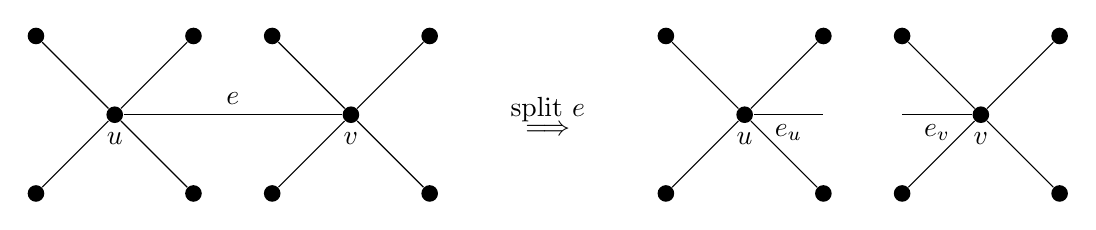
\begin{tikzpicture}
        % Left graph
        \node[circle, fill, inner sep=1pt, minimum size=6pt] (lu) at (0, 0) {};
        \node[circle, fill, inner sep=1pt, minimum size=6pt] (lv) at (3, 0) {};
        \node[circle, fill, inner sep=1pt, minimum size=6pt] (l1) at (-1, 1) {};
        \node[circle, fill, inner sep=1pt, minimum size=6pt] (l2) at (-1, -1) {};
        \node[circle, fill, inner sep=1pt, minimum size=6pt] (l3) at (1, 1) {};
        \node[circle, fill, inner sep=1pt, minimum size=6pt] (l4) at (1, -1) {};
        \node[circle, fill, inner sep=1pt, minimum size=6pt] (l5) at (4, 1) {};
        \node[circle, fill, inner sep=1pt, minimum size=6pt] (l6) at (4, -1) {};
        \node[circle, fill, inner sep=1pt, minimum size=6pt] (l7) at (2, 1) {};
        \node[circle, fill, inner sep=1pt, minimum size=6pt] (l8) at (2, -1) {};
    
        \draw (lu) -- (l1);
        \draw (lu) -- (l2);
        \draw (lu) -- (l3);
        \draw (lu) -- (l4);
        \draw (lu) -- (lv) node[midway, above] {$e$};
        \draw (lv) -- (l5);
        \draw (lv) -- (l6);
        \draw (lv) -- (l7);
        \draw (lv) -- (l8);

        \node at (0, -0.3) {$u$};
        \node at (3, -0.3) {$v$};

        % Arrow
        \node at (5.5, 0) {$\stackrel{\mbox{split $e$}}{\Longrightarrow}$};
    
        % Right graph (left part)
        \node[circle, fill, inner sep=1pt, minimum size=6pt] (ru1) at (8, 0) {};
        \node[circle, fill, inner sep=1pt, minimum size=6pt] (r1) at (7, 1) {};
        \node[circle, fill, inner sep=1pt, minimum size=6pt] (r2) at (7, -1) {};
        \node[circle, fill, inner sep=1pt, minimum size=6pt] (r3) at (9, 1) {};
        \node[circle, fill, inner sep=1pt, minimum size=6pt] (r4) at (9, -1) {};
        % \node[draw, circle, fill=black] (re1) at (7, 0) {};

        \draw (ru1) -- (r1);
        \draw (ru1) -- (r2);
        \draw (ru1) -- (r3);
        \draw (ru1) -- (r4);
        \draw (ru1) -- (9, 0) node[midway, below] {$e_u$};

        \node at (8, -0.3) {$u$};
    
        % Right graph (right part)
        \node[circle, fill, inner sep=1pt, minimum size=6pt] (rv1) at (11, 0) {};
        \node[circle, fill, inner sep=1pt, minimum size=6pt] (r5) at (10, 1) {};
        \node[circle, fill, inner sep=1pt, minimum size=6pt] (r6) at (10, -1) {};
        \node[circle, fill, inner sep=1pt, minimum size=6pt] (r7) at (12, 1) {};
        \node[circle, fill, inner sep=1pt, minimum size=6pt] (r8) at (12, -1) {};
        % \node[draw, circle, fill=black] (re2) at (8, 0) {};

        \draw (rv1) -- (r5);
        \draw (rv1) -- (r6);
        \draw (rv1) -- (r7);
        \draw (rv1) -- (r8);
        \draw (rv1) -- (10, 0) node[midway, below] {$e_v$};

        \node at (11, -0.3) {$v$};
    \end{tikzpicture}
    \caption{an example of splitting the edge $e = \set{u, v}$.}
    \label{fig:splitting-edge}
\end{figure}
    
    \begin{itemize}
    \item Let $G^{(0)} = \left(V, E^{(0)} = E \setminus \set{e} \cup \set{e_u, e_v}\right)$. Let $\Phi^{(0)} = \left(G^{(0)}, \vecf\right)$.
    \item Let $G^{(1)} = \left(V, E^{(1)} = E \setminus \set{e} \cup \set{e_v}\right)$. Let $\vecf^{(1)} \triangleq \set{f_w^{(1)}}_{w \in V}$ where $f_w^{(1)} = f_w$ for each $w \neq u$ and $f_u^{(1)}(i) = f_u(i + 1)$ for each $0 \le i < \deg_G(u)$. Let $\Phi^{(1)} = \left(G^{(1)}, \vecf^{(1)}\right)$.
    \item Let $G^{(2)} = \left(V, E^{(2)} = E \setminus \set{e} \cup \set{e_u}\right)$. Let $\Phi^{(2)} = \left(G^{(2)}, \vecf\right)$.
    \end{itemize}
    Moreover, we have the following properties:
    \begin{itemize}
    \item All of $\Delta\left(G^{(0)}\right), \Delta\left(G^{(1)}\right)$ and $\Delta\left(G^{(2)}\right)$ are no more than $\Delta$;
    \item By $f_u(1)>0$, we have $f_u^{(1)}(i) >0$. Combined with  $\Phi = (G,\vecf)$ satisfies~\Cref{cond:Holant-condition}, one can verify that $\left(\Phi^{(1)},(e_v\leftarrow 1),(e_v\leftarrow 0),v\right)$ satisfies~\Cref{cond-instancepair}.
    Similarly, we have $\left(\Phi^{(2)},(e_u\leftarrow 1),(e_u\leftarrow 0),u\right)$ satisfies~\Cref{cond-instancepair};
    % $\Phi = (G,\vecf)$ satisfies~\Cref{cond:Holant-condition}, one can verify that both $\left(\Phi^{(1)},(e_v\leftarrow 1),(e_v\leftarrow 0),v\right)$ and \\$\left(\Phi^{(2)},(e_u\leftarrow 1),(e_u\leftarrow 0),u\right)$ satisfy~\Cref{cond-instancepair};
    \item Recall the definitions of $r_{\max}$ in \eqref{eq-def-rmax} and $B$ in \eqref{eq-def-bmin}. We have 
    \[r_{\max}(\Phi^{(1)}) = \max_{w \in V} \frac{f^{(1)}_w(1)}{f^{(1)}_w(0)} = \max\left\{\max_{w\neq v} \frac{f_w(1)}{f_w(0)},\frac{f_u(2)}{f_u(1)}\right\} \leq \max\left\{\max_{w\neq v} \frac{f_w(1)}{f_w(0)},\frac{f_u(1)}{f_u(0)}\right\} = r_{\max}(\Phi),\]
    where the inequality is by $f_u$ is log-concave.
    By \eqref{eq:local-polynomial}, we have 
    $P_{f_v}(r_{\max})$

    
    Similarly, we also have $r_{\max}(\Phi^{(2)}) \le r_{\max}(\Phi)$. 
    \end{itemize}
    Set $\varepsilon_1 = \varepsilon_2 = \varepsilon/3$.
    Combined these properties with \Cref{thm:LP-ratio-estimator}, we have that $\wh{R}_1$ can be obtained within time 
    \[\qgl{O\left(\varepsilon_1^{-\poly\left(\Delta(G^{(1)}),1/B\left(\Phi^{(1)}\right)\right)}\right) = O\left(\abs{V} \cdot \varepsilon^{-\poly(\Delta(G),r_{\max}(\Phi))}\right),}\]
    where 
    \begin{align}\label{eq-rhat1}
        (1 - \varepsilon')R_{\Phi^{(1)}}(e_v) \leq \wh{R}_1 \leq (1 + \varepsilon')R_{\Phi^{(1)}}(e_v), 
    \end{align}
    Similarly, $\wh{R}_2$ can be obtained within time 
    \[\qgl{O\left(\abs{V} \cdot \varepsilon_2^{-\poly(\Delta(G^{(2)}),r_{\max}(\Phi^{(2)}))}\right) = O\left(\abs{V} \cdot \varepsilon^{-\poly(\Delta(G),r_{\max}(\Phi))}\right),}\]
    where 
    \begin{align}\label{eq-rhat2}
   (1 - \varepsilon')R_{\Phi^{(2)}}(e_u) \leq \wh{R}_2 \leq (1 + \varepsilon')R_{\Phi^{(2)}}(e_u).
    \end{align}
    Let $\wh{R} = \wh{R}_1 \cdot \wh{R}_2$. 
    Note that
    \begin{equation}\label{eq-rphi-rphi12}
    \begin{aligned}
        R_{\Phi}(e) &= \frac{\Pr[X \sim \mu_{\Phi}]{X(e) = 1}}{\Pr[X \sim \mu_{\Phi}]{X(e) = 0}} \\
        &= \frac{\Pr[X \sim \mu_{\Phi^{(0)}}]{X(e_u) = X(e_v) = 1 \mid X(e_u) = X(e_v)}}{\Pr[X \sim \mu_{\Phi^{(0)}}]{X(e_u) = X(e_v) = 0 \mid X(e_u) = X(e_v)}} \\
        &= \frac{\Pr[X \sim \mu_{\Phi^{(0)}}]{X(e_u) = X(e_v) = 1}}{\Pr[X \sim \mu_{\Phi^{(0)}}]{X(e_u) = X(e_v) = 0}} \\
        &= \frac{\Pr[X \sim \mu_{\Phi^{(0)}}]{X(e_u) = 1 \land X(e_v) = 1}}{\Pr[X \sim \mu_{\Phi^{(0)}}]{X(e_u) = 1 \land X(e_v) = 0}} \cdot \frac{\Pr[X \sim \mu_{\Phi^{(0)}}]{X(e_u) = 1 \land X(e_v) = 0}}{\Pr[X \sim \mu_{\Phi^{(0)}}]{X(e_u) = 0 \land X(e_v) = 0}} \\
        &= \frac{\Pr[X \sim \mu_{\Phi^{(0)}}]{X(e_v) = 1 \mid X(e_u) = 1}}{\Pr[X \sim \mu_{\Phi^{(0)}}]{X(e_v) = 0 \mid X(e_u) = 1}} \cdot \frac{\Pr[X \sim \mu_{\Phi^{(0)}}]{X(e_u) = 1 \mid X(e_v) = 0}}{\Pr[X \sim \mu_{\Phi^{(0)}}]{X(e_u) = 0 \mid X(e_v) = 0}} \\
        &= \frac{\Pr[X \sim \mu_{\Phi^{(1)}}]{X(e_v) = 1}}{\Pr[X \sim \mu_{\Phi^{(1)}}]{X(e_v) = 0}} \cdot \frac{\Pr[X \sim \mu_{\Phi^{(2)}}]{X(e_u) = 1}}{\Pr[X \sim \mu_{\Phi^{(2)}}]{X(e_u) = 0}} \\
        &= R_{\Phi^{(1)}}(e_v) \cdot R_{\Phi^{(2)}}(e_u).
    \end{aligned}
    \end{equation}
    We emphasize that all the denominators in above inequalities are not $0$ because all of $f_u(0),f_v(0), f_u(1),f_v(1)$ are larger than $0$.
    Thus, we have
    \begin{align*}
        \wh{R} &= \wh{R}_1 \cdot \wh{R}_2\\
        \left(\text{by \eqref{eq-rhat1} and \eqref{eq-rhat1}}\right)\quad&\ge (1 - \varepsilon_1)\cdot(1 - \varepsilon_2)\cdot R_{\Phi^{(1)}}(e_v) \cdot R_{\Phi^{(2)}}(e_u) \\
        \left(\text{by $\varepsilon_1 = \varepsilon_2 =\varepsilon/3$}\right) \quad &=         (1 - \varepsilon/3)^2 \cdot R_{\Phi^{(1)}}(e_v) \cdot R_{\Phi^{(2)}}(e_u) \\
       \left(\text{by $\epsilon\in (0,1/4)$ and \eqref{eq-rphi-rphi12}}\right)\quad & \ge (1 - \varepsilon) R_{\Phi}(e).
    \end{align*}
    Similarly, we also have 
    $\wh{R} \le (1 + \varepsilon) R_{\Phi}(e)$. 
    In summary, we have $(1 - \varepsilon) R_{\Phi}(e) \le \wh{R} \le (1 + \varepsilon) R_{\Phi}(e)$. 
    
    
    \qgl{At last, we consider the time cost for calculating $\wh{R}$.
    One can verify that the time cost for constructing $\Phi^{(1)}$ and $\Phi^{(2)}$ is $O(\abs{V}\cdot \Delta(G))$.
    Recall that the time cost for calculating $\wh{R}_1$ and $\wh{R}_2$ is 
    $O\left(\abs{V} \cdot \varepsilon^{-\poly(\Delta(G),r_{\max}(\Phi))}\right)$.
    In summary, the total time cost for calculating $\wh{R}$ is 
    $ O\left(n \cdot \varepsilon^{-\poly(\Delta(G),r_{\max}(\Phi))}\right)$.
    The theorem is proved.}
\end{proof}

% \begin{proof}[Proof of~\Cref{thm:Holant-marginal-estimator}]
%     Firstly we show how to design an estimator for the marginal ratio in the instance $\Phi$ satisfying~\Cref{cond:Holant-condition} by the algorithm in~\Cref{thm:Holant-marginal-ratio-estimator}, and then approximate the marginal probability via this ratio estimator.

%     Given an instance $(\Phi = (G, \vecf), \Delta, r)$ satisfying~\Cref{cond:Holant-condition} and an edge $e = \set{u, v} \in E(G)$, when $f_u(1) = 0$ or $f_v(1) = 0$, it holds that $R_\Phi(e) = 0$ and nothing remains to do. Otherwise $\Pr[X \sim \mu_\Phi]{X(e) = 1} > 0$. Now we split $e$ into two half-edges and construct two instances satisfying~\Cref{cond-instancepair}. Formally speaking, let $e_u = \set{u}$ and $e_v = \set{v}$ be two half-edges. Let $G^{(0)} = \left(V(G), E^{(0)} = E(G) \setminus \set{e} \cup \set{e_u, e_v}\right)$, $G^{(1)} = \left(V(G), E^{(1)} = E(G) \setminus \set{e} \cup \set{e_v}\right)$ and $G^{(2)} = \left(V(G), E^{(2)} = E(G) \setminus \set{e} \cup \set{e_u}\right)$. Then we know that $\Delta(G^{(0)}), \Delta(G^{(1)})$ and $\Delta(G^{(2)})$ are at most $\Delta$.

% \begin{figure}[htbp]
%     \centering
%     \begin{tikzpicture}
%         % Left graph
%         \node[circle, fill, inner sep=1pt, minimum size=6pt] (lu) at (0, 0) {};
%         \node[circle, fill, inner sep=1pt, minimum size=6pt] (lv) at (3, 0) {};
%         \node[circle, fill, inner sep=1pt, minimum size=6pt] (l1) at (-1, 1) {};
%         \node[circle, fill, inner sep=1pt, minimum size=6pt] (l2) at (-1, -1) {};
%         \node[circle, fill, inner sep=1pt, minimum size=6pt] (l3) at (1, 1) {};
%         \node[circle, fill, inner sep=1pt, minimum size=6pt] (l4) at (1, -1) {};
%         \node[circle, fill, inner sep=1pt, minimum size=6pt] (l5) at (4, 1) {};
%         \node[circle, fill, inner sep=1pt, minimum size=6pt] (l6) at (4, -1) {};
%         \node[circle, fill, inner sep=1pt, minimum size=6pt] (l7) at (2, 1) {};
%         \node[circle, fill, inner sep=1pt, minimum size=6pt] (l8) at (2, -1) {};
    
%         \draw (lu) -- (l1);
%         \draw (lu) -- (l2);
%         \draw (lu) -- (l3);
%         \draw (lu) -- (l4);
%         \draw (lu) -- (lv) node[midway, above] {$e$};
%         \draw (lv) -- (l5);
%         \draw (lv) -- (l6);
%         \draw (lv) -- (l7);
%         \draw (lv) -- (l8);

%         \node at (0, -0.3) {$u$};
%         \node at (3, -0.3) {$v$};

%         % Arrow
%         \node at (5.5, 0) {$\stackrel{\mbox{split $e$}}{\Longrightarrow}$};
    
%         % Right graph (left part)
%         \node[circle, fill, inner sep=1pt, minimum size=6pt] (ru1) at (8, 0) {};
%         \node[circle, fill, inner sep=1pt, minimum size=6pt] (r1) at (7, 1) {};
%         \node[circle, fill, inner sep=1pt, minimum size=6pt] (r2) at (7, -1) {};
%         \node[circle, fill, inner sep=1pt, minimum size=6pt] (r3) at (9, 1) {};
%         \node[circle, fill, inner sep=1pt, minimum size=6pt] (r4) at (9, -1) {};
%         % \node[draw, circle, fill=black] (re1) at (7, 0) {};

%         \draw (ru1) -- (r1);
%         \draw (ru1) -- (r2);
%         \draw (ru1) -- (r3);
%         \draw (ru1) -- (r4);
%         \draw (ru1) -- (9, 0) node[midway, below] {$e_u$};

%         \node at (8, -0.3) {$u$};
    
%         % Right graph (right part)
%         \node[circle, fill, inner sep=1pt, minimum size=6pt] (rv1) at (11, 0) {};
%         \node[circle, fill, inner sep=1pt, minimum size=6pt] (r5) at (10, 1) {};
%         \node[circle, fill, inner sep=1pt, minimum size=6pt] (r6) at (10, -1) {};
%         \node[circle, fill, inner sep=1pt, minimum size=6pt] (r7) at (12, 1) {};
%         \node[circle, fill, inner sep=1pt, minimum size=6pt] (r8) at (12, -1) {};
%         % \node[draw, circle, fill=black] (re2) at (8, 0) {};

%         \draw (rv1) -- (r5);
%         \draw (rv1) -- (r6);
%         \draw (rv1) -- (r7);
%         \draw (rv1) -- (r8);
%         \draw (rv1) -- (10, 0) node[midway, below] {$e_v$};

%         \node at (11, -0.3) {$v$};
%     \end{tikzpicture}
%     \caption{an example of splitting the edge $e = \set{u, v}$.}
%     \label{fig:splitting-edge}
% \end{figure}
    
%     Now we consider the following three instances:
%     \begin{itemize}
%         \item $\Phi^{(0)} = \left(G^{(0)}, \vecf\right)$.
%         \item $\Phi^{(1)} = \left(G^{(1)}, \vecf^{(1)}\right)$ where $\vecf^{(1)} = \set{f_w^{(1)}}_{w \in V}$ is constructed as $f_w^{(1)} = f_w$ for $w \neq u$ and $f_u^{(1)}(i) = f_u(i + 1)$ for every $0 \le i < \deg_G(u)$.
%         \item $\Phi^{(2)} = \left(G^{(2)}, \vecf\right)$.
%     \end{itemize}
%     Note that $f_u^{(1)}(1)$ might be $0$. In this case $f_u^{(1)}(i) = 0$ for every $1 \le i < \deg_G(u)$ since $f_u$ is positive log-concave. And we can safely remove $u$ and edges incident to $u$ from $G^{(1)}$ and the marginal ratio in $\Phi^{(1)}$ keeps invariant.
%     Assume that $\Phi^{(1)}$ is the Holant instance after necessary removal. By definition, we have $\Phi^{(1)}$ and $\Phi^{(2)}$ both satisfy~\Cref{cond-instancepair} and $r_{\max}(\Phi^{(1)}) \le r$, $r_{\max}(\Phi^{(2)}) \le r$. By computation,
%     \begin{align*}
%         R_{\Phi}(e) &= \frac{\Pr[X \sim \mu_{\Phi}]{X(e) = 1}}{\Pr[X \sim \mu_{\Phi}]{X(e) = 0}} \\
%         &= \frac{\Pr[X \sim \mu_{\Phi^{(0)}}]{X(e_u) = X(e_v) = 1 \mid X(e_u) = X(e_v)}}{\Pr[X \sim \mu_{\Phi^{(0)}}]{X(e_u) = X(e_v) = 0 \mid X(e_u) = X(e_v)}} \\
%         &= \frac{\Pr[X \sim \mu_{\Phi^{(0)}}]{X(e_u) = X(e_v) = 1}}{\Pr[X \sim \mu_{\Phi^{(0)}}]{X(e_u) = X(e_v) = 0}} \\
%         &= \frac{\Pr[X \sim \mu_{\Phi^{(0)}}]{X(e_u) = 1 \land X(e_v) = 1}}{\Pr[X \sim \mu_{\Phi^{(0)}}]{X(e_u) = 1 \land X(e_v) = 0}} \cdot \frac{\Pr[X \sim \mu_{\Phi^{(0)}}]{X(e_u) = 1 \land X(e_v) = 0}}{\Pr[X \sim \mu_{\Phi^{(0)}}]{X(e_u) = 0 \land X(e_v) = 0}} \\
%         &= \frac{\Pr[X \sim \mu_{\Phi^{(0)}}]{X(e_v) = 1 \mid X(e_u) = 1}}{\Pr[X \sim \mu_{\Phi^{(0)}}]{X(e_v) = 0 \mid X(e_u) = 1}} \cdot \frac{\Pr[X \sim \mu_{\Phi^{(0)}}]{X(e_u) = 1 \mid X(e_v) = 0}}{\Pr[X \sim \mu_{\Phi^{(0)}}]{X(e_u) = 0 \mid X(e_v) = 0}} \\
%         &= \frac{\Pr[X \sim \mu_{\Phi^{(1)}}]{X(e_v) = 1}}{\Pr[X \sim \mu_{\Phi^{(1)}}]{X(e_v) = 0}} \cdot \frac{\Pr[X \sim \mu_{\Phi^{(2)}}]{X(e_u) = 1}}{\Pr[X \sim \mu_{\Phi^{(2)}}]{X(e_u) = 0}} \\
%         &= R_{\Phi^{(1)}}(e_v) \cdot R_{\Phi^{(2)}}(e_u).
%     \end{align*}
%     Now we get an $\varepsilon/2$-approximation to $R_\Phi(e)$ with $\+A_\bot$ in~\Cref{thm:Holant-marginal-ratio-estimator}.
%     Set $\varepsilon' = \varepsilon/6$. We employ $\+A_\bot$ in~\Cref{thm:Holant-marginal-ratio-estimator} to obtain $\varepsilon'$-approximations $\wh{R}_1$ and $\wh{R}_2$ to $R_{\Phi^{(1)}}(e_v)$ and $R_{\Phi^{(2)}}(e_u)$ respectively. Then let $\wh{R} = \wh{R}_1 \cdot \wh{R}_2$. By~\Cref{thm:Holant-marginal-ratio-estimator}, we have that
%     \begin{align*}
%         \wh{R} \ge (1 - \varepsilon/6)^2 R_{\Phi^{(1)}}(e_v) \cdot R_{\Phi^{(2)}}(e_u) \ge (1 - \varepsilon/2) R_{\Phi}(e)
%     \end{align*}
%     and
%     \begin{align*}
%         \wh{R} \le (1 + \varepsilon/6)^2 R_{\Phi^{(1)}}(e_v) \cdot R_{\Phi^{(2)}}(e_u) \le (1 + \varepsilon/2) R_{\Phi}(e).
%     \end{align*}

%     Now we approximate $\Pr[X \sim \mu_{\Phi}]{X(e) = 0}$ from $\wh{R}$. Recall that $\wh{R}$ is an $(\varepsilon/2)$-approximation to $R_{\Phi}(e)$. Since $\Pr[X \sim \mu_{\Phi}]{X(e) = 0} = \frac{1}{1 + R_\Phi(e)}$, set $\wh{P} = \frac{1}{1 + \wh{R}}$ and it holds that
%     \begin{align*}
%         \wh{P} \ge \frac{1}{1 + (1 + \varepsilon/2) R_{\Phi}(e)} \ge \frac{1}{1 + \varepsilon/2} \frac{1}{1 + R_{\Phi}(e)} \ge (1 - \varepsilon) \Pr[X \sim \mu_{\Phi}]{X(e) = 0}
%     \end{align*}
%     and
%     \begin{align*}
%         \wh{P} \le \frac{1}{1 + (1 - \varepsilon/2) R_{\Phi}(e)} \le \frac{1}{1 - \varepsilon/2} \frac{1}{1 + R_{\Phi}(e)} \le (1 + \varepsilon) \Pr[X \sim \mu_{\Phi}]{X(e) = 0}
%     \end{align*}
%     where we use inequalities $\frac{1}{1 + x} \ge 1 - 2x$ for every $x \ge 0$ and $\frac{1}{1 - x} \le 1 + 2x$ for every $0 \le x \le \frac{1}{2}$. Hence we conclude an $\varepsilon$-approximation to the marginal probability.

%     Now we consider the running time. Note that in the estimating process, we only make $2$ calls to $\+A_\bot$ with tolerance error $\varepsilon/6$. Then we can obtain $\wh{P}$ within time $\poly\left((6/\varepsilon)^{C(\Delta, r)}\right) = \poly\left((1/\varepsilon)^{C_{\ref{thm:Holant-marginal-estimator}}}\right)$ where the coefficients of the polynomial and $C_{\ref{thm:Holant-marginal-estimator}}$ depend only on $\Delta$ and $r$.
% \end{proof}

\section{Approximate Counting}

Now we give our deterministic algorithm to approximately count the partition function of instances satisfying~\Cref{cond:Holant-condition} via the marginal ratio estimator in~\Cref{thm:Holant-marginal-ratio-estimator}.

\begin{proof}[Proof of~\Cref{thm:counting-Holant}]
    Without loss of generality, assume that $\varepsilon < 1/4$, $\abs{E} = m$ and $E = \{E = e_1, \ldots, e_m\}$. For each $ i \in [m + 1]$, define $G_i \triangleq (V, E_i)$ where $E_i = E \setminus \set{e_1, \ldots, e_{i - 1}}$ 
    and $\Phi_i \triangleq (G_i, \vecf)$. We remark that $G_1 = G$, $G_{m + 1} = (V, \emptyset)$ and $\Delta(G_i)\leq \Delta(G)$ for each $i\in [m+1]$.     
    By $\Phi$ satisfies~\Cref{cond:Holant-condition}, we also have 
    $\Phi_i$ satisfies~\Cref{cond:Holant-condition} for each $i \in [m+1]$. 
    Thus, we have 
    \begin{equation}
    \begin{aligned}\label{eq-z-decompose}
        Z_{\Phi} &= Z_{\Phi}^{e_1 \gets 0} + Z_{\Phi}^{e_1 \gets 1} \\
\left(\text{by \eqref{def-rphie}}\right) \quad       &= \left(1 + R_{\Phi}(e_1)\right) Z_{\Phi}^{e_1 \gets 0} \\
\left(\text{by definitions of $\Phi_1,\Phi_2$}\right) \quad        &= \left(1 + R_{\Phi_1}(e_1)\right) Z_{\Phi_2} \\
        &= \left(1 + R_{\Phi_1}(e_1)\right) \left(Z_{\Phi_2}^{e_2 \gets 0} + Z_{\Phi_2}^{e_2 \gets 1}\right) \\
\left(\text{by \eqref{def-rphie}}\right) \quad        &= \left(1 + R_{\Phi_1}(e_1)\right) \left(1 + R_{\Phi_2}(e_2)\right) Z_{\Phi_2}^{e_2 \gets 0} \\
\left(\text{by definitions of $\Phi_2,\Phi_2$}\right) \quad         &= \left(1 + R_{\Phi_1}(e_1)\right) \left(1 + R_{\Phi_2}(e_2)\right) Z_{\Phi_3} \\
        &= \cdots \\
        &= Z_{\Phi_{m + 1}}\prod_{i = 1}^{m} \left(1 + R_{\Phi_i}(e_i)\right) \\
\left(\text{by $E_{m + 1} = \emptyset$}\right) \quad        &= \prod_{v \in V} f_v(0) \prod_{i = 1}^{m} \left(1 + R_{\Phi_i}(e_i)\right).
    \end{aligned} 
    \end{equation}
For each $1 \le i \le m$, we run the algorithm $\+A$ in~\Cref{thm:Holant-marginal-ratio-estimator} with tolerance error $\varepsilon/(2m)$ on the input $\Phi_i, e_i$ to obtain an $\wh{R}_i$
where 
\begin{align}\label{eq-condition-ri}
(1-\varepsilon/(2m))R_{\Phi_i}(e_i) \leq \wh{R}_i \leq (1+\varepsilon/(2m))R_{\Phi_i}(e_i).
\end{align}
Define 
\begin{align}\label{eq-def-z}
\wh{Z} \triangleq \prod_{v \in V} f_v(0) \prod_{i = 1}^{m} (1 + \wh{R}_i).
\end{align}
Thus, we have 
 \begin{align*}
    &\frac{\wh{Z}}{Z_\Phi} \\
\left(\text{by \eqref{eq-z-decompose} and \eqref{eq-def-z}}\right)\quad    = &\prod_{i = 1}^{m} \left( \frac{1 + \wh{R}_i}{1 + R_{\Phi_i}(e_i)}\right)\\ 
\left(\text{by \eqref{eq-condition-ri}}\right)\quad    \ge &\prod_{i = 1}^{m}  \left( \frac{1+(1-\varepsilon/(2m))R_{\Phi_i}(e_i) }{1 + R_{\Phi_i}(e_i)}\right)\\
 \ge &\prod_{i = 1}^{m} \left(1- \frac{\varepsilon\cdot R_{\Phi_i}(e_i)}{2m(1 + R_{\Phi_i}(e_i))}\right)\\ 
  \ge &\prod_{i = 1}^{m} \left(1- \frac{\varepsilon}{2m}\right)\\
\left(\text{by $\varepsilon\in (0,1/4)$}\right)\quad   \ge & 1 - \varepsilon.
\end{align*}
Similarly, we also have 
\begin{align*}
     &\frac{\wh{Z}}{Z_\Phi} \\
\left(\text{by \eqref{eq-z-decompose} and \eqref{eq-def-z}}\right)\quad    = &\prod_{i = 1}^{m} \left( \frac{1 + \wh{R}_i}{1 + R_{\Phi_i}(e_i)}\right)\\ 
\left(\text{by \eqref{eq-condition-ri}}\right)\quad    \leq &\prod_{i = 1}^{m}  \left( \frac{1+(1+\varepsilon/(2m))R_{\Phi_i}(e_i) }{1 + R_{\Phi_i}(e_i)}\right)
\\ \leq &\prod_{i = 1}^{m} \left(1+ \frac{\varepsilon\cdot R_{\Phi_i}(e_i)}{2m(1 + R_{\Phi_i}(e_i))}\right)\\ 
\leq&\prod_{i = 1}^{m} \left(1+ \frac{\varepsilon}{2m}\right) \\
\left(\text{by $\varepsilon\in (0,1/4)$}\right)\quad\le& 1 + \varepsilon.
\end{align*}

Now we turn to the running time of the algorithm.
Firstly we can obtain $\prod_{v \in V} f_v(0)$ in time $O(\abs{V})$. For every $i \in [m]$, by~\Cref{thm:Holant-marginal-ratio-estimator}, we can obtain $\wh{R}_i$ in time \hktodo{$\poly\left((m/\varepsilon)^{C(\Delta, r)}\right)\leq $}. Hence we can calculate $\wh{Z}$ in time \hktodo{$\poly\left((m/\varepsilon)^{C(\Delta, r)}\right)$}. 
The theorem is proved.
\end{proof}

The algorithm for counting $b$-matchings comes directly from~\Cref{thm:counting-Holant}.

\hktodo{the proof here}
\begin{proof}[Proof of~\Cref{thm:counting-b-matchings}]
    For any graph $G = (V, E)$ and any positive integer $b \le \Delta(G)$, we view $b$-matchings as a Holant instance $\Phi_{G, b} = (G, \vecf)$. Formally speaking, we associate every $v \in V$ with $f_v$ defined as $f_v(i) = \id{i \le b}$ for every $0 \le i \le \Delta$. By definition, the instance $\left(\Phi_{G, b}, \Delta, 1\right)$ satisfies~\Cref{cond:Holant-condition}. Applying~\Cref{thm:counting-Holant} on input $\Phi_{G, b}$ with tolerance error $\varepsilon$, we obtain an $\varepsilon$-approximation to $\abs{\Omega_{G, b}}$ in time $\poly\left((\abs{E} \cdot \varepsilon^{-1})^{C}\right)$ where $C$ depends only on $\Delta$.
\end{proof}

\section{Counterexample}
\zdtodo{move this part to the end of the construction of the coupling tree.}
\zdtodo{mentioned in the introduction and LP section}

In this section, we give a counterexample to show that the updated edge cannot be arbitrarily chosen in the coupling process.

Let $G = (V, E)$ be the graph shown in~\Cref{fig:edge-selection-counterexample} with $V = \set{v_\bot, v_1, v_2, v_3, v_4, v_5}$ and $E = \set{e_1, e_2, e_3, e_4, e_5, e_6, e_\bot}$ consisting of normal edges $e_1 = \{v_\bot, v_1\}, e_2 = \{v_\bot, v_2\}, e_3 = \{v_\bot, v_3\}, e_4 = \{v_1, v_4\}, e_5 = \{v_3, v_5\}, e_6 = \{v_4, v_5\}$ and a half-edge $e_\bot = \set{v_\bot}$.
Let $t$ be a large positive integer which will be picked later. We assign signatures $\vecf = \set{f_v}_{v \in V}$ as $f_{v_\bot} = [1, 1, 1]$, $f_{v_2} = [1, 1]$ and $f_{v_1} = f_{v_3} = f_{v_4} = f_{v_5} = [1, t]$.

\begin{figure}[htbp]
    \centering
    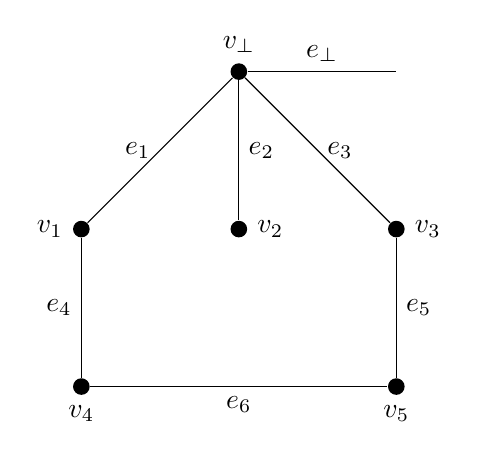
\begin{tikzpicture}
        % Vertices
        \node (v0) at (0, 3) [circle, fill, inner sep=1pt, minimum size=6pt, label=above:$v_\bot$] {};
        \node (v1) at (-2, 1) [circle, fill, inner sep=1pt, minimum size=6pt, label=left:$v_1$] {};
        \node (v2) at (0, 1) [circle, fill, inner sep=1pt, minimum size=6pt, label=right:$v_2$] {};
        \node (v3) at (2, 1) [circle, fill, inner sep=1pt, minimum size=6pt, label=right:$v_3$] {};
        \node (v4) at (-2, -1) [circle, fill, inner sep=1pt, minimum size=6pt, label=below:$v_4$] {};
        \node (v5) at (2, -1) [circle, fill, inner sep=1pt, minimum size=6pt, label=below:$v_5$] {};
        % Edges
        \draw (v0) -- (2, 3) node[midway, above] {$e_{\bot}$};
        \draw (v0) -- (v1) node[midway, left] {$e_1$};
        \draw (v0) -- (v2) node[midway, right] {$e_2$};
        \draw (v0) -- (v3) node[midway, right] {$e_3$};
        \draw (v1) -- (v4) node[midway, left] {$e_4$};
        \draw (v3) -- (v5) node[midway, right] {$e_5$};
        \draw (v4) -- (v5) node[midway, below] {$e_6$};
    \end{tikzpicture}
    \caption{The counterexample of the edge selection.}
    \label{fig:edge-selection-counterexample}
\end{figure}

Let $\sigma = (e_\bot \gets 0)$ and $\tau = (e_\bot \gets 1)$. It is easy to verify that the instance $(\Phi = (G, \vecf), \sigma, \tau, v_\bot)$ satisfies~\Cref{cond-instancepair}. Consider the marginals of $e_2 = \set{v_\bot, v_2}$. By direct calculation, we have $\Ham(\sigma, E_{v_\bot}) < \Ham(\tau, E_{v_\bot})$ and
$$
    \mu_{e_2}^{\sigma}(1) = \frac{t^4 + 4t^3 + 3t^2 + 2t + 1}{3t^4 + 8t^3 + 7t^2 + 4t + 2}, \quad \mu_{e_2}^{\tau}(1) = \frac{t^4 + 3t^2 + 1}{2t^4 + 4t^3 + 6t^2 + 2t + 2}.
$$
Pick $t = 10$, and it holds that
$$
    \mu_{e_2}^{\sigma}(1) = \frac{14321}{38742} < \frac{10301}{24622} = \mu_{e_2}^{\tau}(1),
$$
meaning that there exists an instance $(\Phi, \sigma, \tau, v)$ and an edge $e \in E_v^\sigma$ such that $\Ham(\sigma, E_v) < \Ham(\tau, E_v)$ and $\mu_{e}^{\sigma}(1) < \mu_{e}^{\tau}(1)$.

% Let $G = (V,E)$ with $V  = \{v_0,v_1,v_2,v_3,v_4,v_5\}$
% and $E=\{e_1,e_2,e_3,e_4,e_5,e_6\}$ where 
% % $e_1 = \{v_0,v_1\},e_2 = \{v_0,v_2\},e_3 = \{v_0,v_3\},e_4 = \{v_1,v_4\},e_5 = \{v_3,v_5\},e_6=\{v_4,v_5\}$.
% Moreover, let $t$ be a large integer.
% $f_{v_0} = [1,1,1]$, $f_{v_2} = [1,1]$,
% $f_{v_1} = f_{v_3} = f_{v_4} = f_{v_5} = [1,t]$.

% One can verify that only three subgraphs of $G$ with a weight larger than $t^4$.

% The first one is the graph 
% $G_1 = (V,E_1)$ where $E_1 = (e_1,e_3,e_6)$. And the weight is $t^4$.

% The second one is the graph 
% $G_2 = (V,E_2)$ where $E_2 = (e_4,e_5)$. And the weight is $t^4$.

% The second one is the graph 
% $G_3 = (V,E_3)$ where $E_2 = (e_2,e_4,e_5)$. And the weight is $t^4$.

% When $t$ goes into infinity, only these three subgraphs are valid.
% Thus, the probability that the edge $e_2$ occurs is 1/3.

% Consider another $f'_{v_0} = [1,1]$.
% One can verify that when $t$ goes into infinity, only $G_2$ and $G_3$ are valid.
% Thus, the probability that the edge $e_2$ occurs is 1/2,
% larger than 1/3.

% In the first instance:
% $$
%     \mu^{e_\bot = 0}_{e_2}(1) = \frac{t^4 + 4t^3 + 3t^2 + 2t + 1}{3t^4 + 8t^3 + 7t^2 + 4t + 2}
% $$
% while in the second instance:
% $$
%     \mu^{e_\bot = 1}_{e_2}(1) = \frac{t^4 + 3t^2 + 1}{2t^4 + 4t^3 + 6t^2 + 2t + 2}.
% $$

\bibliographystyle{alpha}
\bibliography{refs}

\appendix

\section{Proofs for Properties of Holant Instances} \label{sec:proof-Holant-properties}

Now we complete the deferred proofs for properties of Holant instances. Recall that $\Phi = (G = (V, E = E_1 \cup E_2), \vecf = \set{f_v})$ is a binary symmetric log-concave Holant instance satisfying~\Cref{cond:Holant-condition} and $\mu = \mu_\Phi$ is its Gibbs distribution.

\subsection{Feasibility of partial assignments}

We recall the theorem for the feasibility of partial assignments.
\PartialFeasibility*

To show the feasibility of a partial assignment $\sigma$, we first make the following claim.
\begin{claim} \label{claim:partial-assignment-feasibility}
    A partial assignment $\sigma$ is feasible if and only if the assignment $\sigma'$ on $E$ is feasible where $\sigma'$ is defined as
    \begin{align} \label{eq:0-assignment}
        \sigma'(e) = \begin{cases}
            \sigma(e) & \sigma \in \Lambda(\sigma) \\
            0 & \mbox{otherwise}
        \end{cases}\;.
    \end{align}
\end{claim}
\begin{proof}
    When $\sigma'$ is feasible, obviously $\sigma$ is feasible since $\sigma' \in \sigma$. To see the other side, when $\sigma$ is feasible, there exists $\tau : E \to \set{0, 1}$, $\tau \in \sigma$ such that $\mu(\tau) > 0$. Hence we have $\prod_{v \in V} f_v\left(\abs{\tau(E_v)}\right) > 0$ meaning that $f_v\left(\abs{\tau(E_v)}\right) > 0$ for every $v \in V$. Since $f_v$ is log-concave, $f_v(0) > 0$ and $\abs{\sigma'(E_v)} \le \abs{\tau(E_v)}$, it holds that $f_v\left(\abs{\sigma'(E_v)}\right) > 0$. Therefore we obtain that $\mu(\sigma') > 0$ by the definition of $\mu(\sigma')$.
\end{proof}

\begin{proof}[Proof of~\Cref{lem:partial-assignment-feasibility}]
    By~\Cref{claim:partial-assignment-feasibility}, we check the feasibility of $\sigma'$ defined as~\eqref{eq:0-assignment}. In other words, we check whether $f\left(\abs{\sigma'(E_v)}\right) > 0$ for every $v \in V$. By definition, for every $v \in V$, $\abs{\sigma'(E_v)} = \Ham(\sigma, v)$ and thus $f\left(\abs{\sigma'(E_v)}\right) = f\left(\Ham(\sigma, v)\right)$. When $\Lambda(\sigma) \cap E_v = \emptyset$, we need to do nothing from the assumption $f_v(0) > 0$. Let $V(\sigma) \defeq \set{v \in V \cmid \Lambda(\sigma) \cap E_v \neq \emptyset}$. It is not hard to see that we can find $V(\sigma)$ and compute $\Ham(\sigma, v)$ for every $v \in V(\sigma)$ in time $O(\abs{\Lambda(\sigma)})$ by enumerating all edges in $\Lambda(\sigma)$. Hence we can check the feasibility of a partial assignment $\sigma$ in time $O(\abs{\Lambda(\sigma)})$. 
\end{proof}

\subsection{Marginal ratio bounds}

In this part, we prove the upper bound for marginal ratios.

% \MarginalBound*
\MarginalRatioBound*
\begin{proof}
    Let $v$ be the unique vertex incident to $e$. Since $f_v$ is log-concave and $f_v(0) > 0$, it holds that $f_v(i + 1) \le r_{\max}(\Phi) f_v(i)$. Hence we have, for every $\sigma \in \set{0, 1}^E$ with $\sigma(e) = 1$, $\prod_{u \in V} f_u\left(\abs{\sigma(E_u)}\right) \le r_{\max}(\Phi) \prod_{u \in V} f_u\left(\abs{\sigma'(E_u)}\right)$ where $\sigma'(e') = \sigma(e')$ for every $e' \in E \setminus \set{e}$ and $\sigma'(e) = 0$. Then by direct calculation,
    \begin{align*}
        R_{\Phi}(e) &= \frac{Z_{\Phi}^{e \gets 1}}{Z_{\Phi}^{e \gets 0}} \\
        &= \frac{\sum_{\sigma \in \set{0, 1}^E : \sigma(e) = 1} \prod_{u \in V} f_u\left(\abs{\sigma(E_u)}\right)}{\sum_{\sigma \in \set{0, 1}^E : \sigma(e) = 0} \prod_{u \in V} f_u\left(\abs{\sigma(E_u)}\right)} \\
        &\le \frac{r_{\max}(\Phi) \sum_{\sigma \in \set{0, 1}^E : \sigma(e) = 0} \prod_{u \in V} f_u\left(\abs{\sigma(E_u)}\right)}{\sum_{\sigma \in \set{0, 1}^E : \sigma(e) = 0} \prod_{u \in V} f_u\left(\abs{\sigma(E_u)}\right)} \le r_{\max}(\Phi).
    \end{align*}
    Then we conclude the upper bound.
\end{proof}

\section{Omitted proofs}\label{sec:omitted Proofs}

% \OneroundDecay*
% \begin{proof}
% Let $\ell$ denote $\abs{E_v^\sigma}$. 
% % Let $\ell$ denote the number of times the while loop is executed in $\!{Couple}(\Phi, \sigma, \tau, v)$.
% % We remark that $\ell$ is a random variable.
% For each $i>0$,
% let $e_i, \sigma_i,\tau_i,\sigma_{e_i},\tau_{e_i}$ be the random variables $e,\sigma,\tau,\sigma_{e},\tau_{e}$ in Line \ref{line-edge-sample} of the $i$-th iteration of the while loop, respectively.
% Let $\+E$ denote the event that 
% $\land_{i\in [\ell]}(\sigma_{e_i} = \tau_{e_i} = ( e_i\leftarrow 0))$.
% We remark that this event is well-defined.
% Because for each $1< i \leq \ell$,
% under the condition that $\sigma_{e_{i-1}} = \tau_{e_{i-1}} = (e_{i-1}\leftarrow 0)$, Line \ref{line-recursive-call} of Algorithm \ref{algo:Couple} is skiped.
% In addition, we have $E^{\sigma_{i}}_v\neq \emptyset$, because only $i-1<\ell$ edges in $E_v^\sigma$ are assigned in $\sigma_{i}$.
% Thus, the $i$-th iteration of the while loop must be performed
% and $\sigma_{e_i}$ and $\tau_{e_i}$ are well-defined.
% Therefore, $\+E$ is also well-defined.


% For any $1<i\leq  \ell$, under the condition $\left(\sigma_{e_{1}}=\tau_{e_{1}} = (e_1\leftarrow 0)\right)\land \cdots\land \left(\sigma_{e_{i-1}} = \tau_{e_{i-1}}=(e_{i-1}\leftarrow 0)\right)$,
% we have $\!{Ham}\left(\sigma_i, {E_v}\right) = \!{Ham}\left(\sigma, {E_v}\right) > \!{Ham}\left(\tau, {E_v}\right) = \!{Ham}\left(\tau_i, {E_v}\right)$.
% Thus, we have $e_i$ satisfies 
%                     $\mu^{\sigma_i}_e(1) \leq \mu^{\tau_i}_e(1)$
% by Line \ref{line:pick-dominating-edge-2} of Algorithm \ref{algo:Couple}.
% Therefore, $\mu^{\sigma_i}_e(0) = 1 - \mu^{\sigma_i}_e(1) \geq 1 - \mu^{\tau_i}_e(1)  = \mu^{\tau_i}_e(0)$.
% Moreover, according to Line \ref{line-edge-sample},
% we have 
% $(\sigma_{e_i}, \tau_{e_i})$ is sampled from an optimal coupling of $(\mu^{\sigma_i}_{e_i}, \mu^{\tau_i}_{e_i})$.
% Thus, we have 
% \begin{align*}
% &\symbolwidth \Pr{\sigma_{e_{i}} = \tau_{e_{i}} = (e_i\leftarrow 0)\mid \left(\sigma_{e_{1}}=\tau_{e_{1}} = (e_1\leftarrow 0)\right)\land \cdots\land \left(\sigma_{e_{i-1}} = \tau_{e_{i-1}}=(e_{i-1}\leftarrow 0)\right)}
% \\
% &= \min\left\{\mu^{\sigma_i}_e(0), \mu^{\tau_i}_e(0)\right\} = \mu^{\tau_i}_e(0),
% \end{align*}
% where the last inequality is by $\mu^{\sigma_i}_e(0) \geq \mu^{\tau_i}_e(0)$.
% Similarly, one can also prove that 
% \begin{align*}
% \Pr{\sigma_{e_{1}} = \tau_{e_{1}} = (e_1\leftarrow 0)} = \mu^{\tau_1}_e(0) = \mu^{\tau}_e(0).
% \end{align*}
% Therefore, we have 
% \begin{equation*}
% \begin{aligned}
% &\symbolwidth \Pr{\+E} = \prod_{i\in [\ell]}\Pr{\sigma_{e_{i}} = \tau_{e_{i}} = (e_i\leftarrow 0)\mid \left(\sigma_{e_{1}}=\tau_{e_{1}} = (e_1\leftarrow 0)\right)\land \cdots\land \left(\sigma_{e_{i-1}} = \tau_{e_{i-1}}=(e_{i-1}\leftarrow 0)\right)}
% \\
% &= \prod_{i\in [\ell]}\mu^{\tau_i}_{e_i}(0)
% =\mu^{\tau}_{e_1}(0)\cdot \mu^{\tau\land (e_1\leftarrow 0)}_{e_2}(0)\cdots \mu^{\tau\land (e_1\leftarrow 0)\cdots\land (e_{\ell-1}\leftarrow 0)}_{e_{\ell}}(0)
% = \mu_{E_v^\tau}^{\tau}(\zero)
% \geq  B(\Phi),
% \end{aligned}
% \end{equation*}
% where the last inequality is by \Cref{lem:marginal-bound}.
% In addition, we claim that if $\+E$ happens, then $\!{Couple}(\cdot)$ is not called in $\!{Couple}(\Phi, \sigma, \tau, v)$.
% Thus, we have 
% \begin{equation*}
% \begin{aligned}
% &\symbolwidth\Pr{\!{Couple}(\cdot) \text{ is recursively called in Line \ref{line-recursive-call} of $\!{Couple}(\Phi, \sigma, \tau, v)$}}
% \\&=1-\Pr{\!{Couple}(\cdot) \text{ is never called in Line \ref{line-recursive-call} of $\!{Couple}(\Phi, \sigma, \tau, v)$}}
% \\&\leq 1- \Pr{\+E}
% \\&\leq 1- B(\Phi).
% \end{aligned}
% \end{equation*}

% At last, we prove the claim that $\!{Couple}(\cdot)$ is not called in $\!{Couple}(\Phi, \sigma, \tau, v)$ if $\+E$ happens.
% Then the lemma is immediate.
% Assume $\+E$ happens.
% We have $\sigma_{e_i} = \tau_{e_i}$ for each $i\in [\ell]$,
% Then Line \ref{line-recursive-call} of Algorithm \ref{algo:Couple} is skiped in the $i$-th iteration of the while loop.
% {Moreover, we have $E^{\sigma_{\ell}\land \sigma_{e_\ell}}_v=\emptyset$, because all the edges 
% $e_1,\cdots,e_{\ell}$ in $E_v^\sigma$ are assigned in $\sigma_{\ell}\land \sigma_{e_\ell}$.}
% Thus, the $(\ell+1)$-th iteration of the while loop will not be performed.
% Thus, $\!{Couple}(\cdot)$ in Line \ref{line-recursive-call} is never called in $\!{Couple}(\Phi, \sigma, \tau, v)$.
% The claim is proved, which finishes the proof of the lemma.


% \end{proof}


\PropertyDefrpc*
\begin{proof}
To prove this lemma, it is sufficient to prove that for each $(\sigma, \tau, \seqS,v,t)$,
\begin{align}\label{eq-def-trp-perperty-sigma-delete-vt}
\Pr[\!{cp}]{(\sigma, \tau, \seqS,v,t)}\leq \mu^{\sigma_{\bot}}_{\seqS}(\sigma).
\end{align}
Similarly, one can also prove that $\Pr[\!{cp}]{(\sigma, \tau, \seqS,v,L)}\leq \mu^{\tau_{\bot}}_{\seqS}(\tau)$.
Thus, \eqref{eq-def-trp-perperty-sigma} is proved.
Meanwhile, for each $e\in E^{\sigma}_v$,
by \Cref{def-notation-trp} and \eqref{eq-def-trp-perperty-sigma-delete-vt}, 
we have
\begin{align*}
\Pr[\!{cp}]{(\sigma, \tau, \seqS,v,L,e)} \leq  \Pr[\!{cp}]{(\sigma, \tau, \seqS,v,L)} \leq \mu^{\sigma_{\bot}}_{\seqS}(\sigma).
\end{align*}
Similarly, one can also prove that $\Pr[\!{cp}]{(\sigma, \tau, \seqS,v,L,e)}\leq \mu^{\tau_{\bot}}_{\seqS}(\tau)$.
Thus, \eqref{eq-def-trp-perperty-sigma-e} is also proved and the lemma is immediate.

In the following, we prove \eqref{eq-def-trp-perperty-sigma-delete-vt} by induction on the length of $\seqS$.
The induction basis is when $\seqS = \varnothing$.
In this case, by \eqref{eq-def-pro-stsvl} we have 
\begin{align*}
 \Pr[\!{cp}]{(\sigma, \tau, \seqS,v,L)} = \Pr{\left(T\geq 0\right)\land \left((\sigma, \tau, \seqS, v, L) = (\sigma_\bot, \tau_\bot, \varnothing, v_\bot, 0)\right)}\leq 1 = \mu^{\sigma_{\bot}}_{\seqS}(\sigma).
\end{align*}
% If $\sigma = \sigma_\bot$, we have 
% \begin{align*}
%  \Pr[\!{cp}]{(\sigma, \tau, \seqS, v, L)} \leq 1 = \mu^{\sigma_{\bot}}_{\seqS}(\sigma).
% \end{align*}
% Otherwise, $\sigma \neq \sigma_\bot$. We have 
% \begin{align*}
%  \Pr[\!{cp}]{(\sigma, \tau, \seqS, v, L)} = 0 \leq \Pr[X \sim \mu]{X \in \sigma \mid X(e_\bot) = 1}.
% \end{align*}
The base case is proved. For the induction step,  assume $\abs{\seqS} = t>0$, $\seqS = \seqS'\circ e$, $\sigma = \sigma'\land(e\leftarrow a)$, $\tau = \tau'\land(e\leftarrow b)$ for some $e\in E(G),a,b\in \{0,1\}$.
By \eqref{eq-def-pro-stsvl} we have 
\begin{align*}
 \Pr[\!{cp}]{(\sigma, \tau, \seqS, v, L)} 
 = \Pr{\left(T\geq t\right)\land \left((\sigma, \tau, \seqS, v, L) = (\sigma_t, \tau_t, \seqS_t, v_t, L_t)\right)}.
\end{align*}
In addition, by \Cref{def:truncated-random-process},
we have the event $\left(T\geq t\right)\land \left((\sigma, \tau, \seqS, v, L) = (\sigma_t, \tau_t, \seqS_t, v_t, L_t)\right)$ happens only if 
\begin{itemize}
\item the event $\+E\triangleq \left(T\geq t-1\right)\land \left((\sigma', \tau', \seqS', v(\sigma',\tau'), L(\sigma',\tau')) = (\sigma_{t-1}, \tau_{t-1}, \seqS_{t-1}, v_{t-1}, L_{t-1})\right)$ happens;
\item the chosen edge in the state $(\sigma_{t-1}, \tau_{t-1}, \seqS_{t-1}, v_{t-1}, L_{t-1})$ is $e$ and the sample $(\sigma_e,\tau_e)$ from an optimal coupling of $(\mu_e^{\sigma_{t-1}},\mu_e^{\tau_{t-1}})$ is $(a,b)$.
\end{itemize}
Thus, we have
\begin{align*}
 &\symbolwidth \Pr[\!{cp}]{(\sigma, \tau, \seqS, v, L)}\\ 
 &= \Pr{\left(T\geq t\right)\land \left((\sigma, \tau, \seqS, v, L) = (\sigma_t, \tau_t, \seqS_t, v_t, L_t)\right)}\\
&\leq 
\Pr{\+E}\cdot\Pr{(\sigma_e,\tau_e) =(a,b)\mid \+E}
\\&\leq \Pr{\left(T\geq t-1\right)\land \left((\sigma', \tau', \seqS', v(\sigma',\tau'), L(\sigma',\tau')) = (\sigma_{t-1}, \tau_{t-1}, \seqS_{t-1}, v_{t-1}, L_{t-1})\right)}\cdot\Pr{(\sigma_e,\tau_e) =(a,b)\mid \+E}
\\&\leq \mu^{\sigma_{\bot}}_{\seqS'}(\sigma')\cdot\Pr{(\sigma_e,\tau_e) =(a,b)\mid \+E},
\end{align*}
where the last inequality is by the induction hypothesis.
Moreover, we have 
\begin{equation*}
\begin{aligned}
\Pr{(\sigma_e,\tau_e) =(a,b)\mid \+E}
\leq \Pr{\sigma_e =a\mid \+E}
= \mu_e^{\sigma_{t-1}}\left(a \mid \+E\right)
= \mu_e^{\sigma'}(a),
\end{aligned}
\end{equation*}
where the first equality is by $(\sigma_e,\tau_e)$ is a coupling of $(\mu_e^{\sigma_{t-1}},\mu_e^{\tau_{t-1}})$ and the second equality is by $\sigma_{t-1} = \sigma'$ if $\+E$ happens.
Therefore, we have 
\begin{align*}
\Pr[\!{cp}]{(\sigma, \tau, \seqS, v, L)}\leq \mu^{\sigma_{\bot}}_{\seqS'}(\sigma')\cdot \mu_e^{\sigma'}(a) = \mu^{\sigma_{\bot}}_{\seqS}(\sigma).
\end{align*}
This completes the induction step.
Then \eqref{eq-def-trp-perperty-sigma-delete-vt} is proved and the lemma is immediate.
\end{proof}


\PropertyTruncateTree*

\begin{proof}
    \underline{Proof of (1).} By \Cref{def:truncated-coupling-tree},  each infeasible node is a leaf in $\+T$.
    Formally, $V(\+T) \setminus \+V \subseteq \+L$.
    Thus,  $V(\+T) \setminus \+L \subseteq \+V$.
    Therefore, $V(\+T) \setminus \+L \subseteq \+V\setminus \+L$.
    Combined with $\+V\subseteq V(\+T)$, we have $V(\+T) \setminus \+L = \+V\setminus \+L$.
    \vspace{0.2cm}
    
    \underline{Proof of (2).} 
    Let $(\sigma_0,\tau_0,\seqS_0,v_0,L_0),\cdots,(\sigma_t,\tau_t,\seqS_t,v_t,L_t)$ be a path from the root to any leaf in $\+T$, where $(\sigma_0,\tau_0,\seqS_0,v_0,L_0)$ is the root $(\sigma_\bot, \tau_\bot, \varnothing, v_\bot, 0)$ and $(\sigma_t,\tau_t,\seqS_t,v_t,L_t)$ is the leaf.
    At first, we prove the bound on the depth of $\+T$.
    According to ~\Cref{def:truncated-coupling-tree}, for each $0\leq i <t$, one can verify that either $L_{i+1}= L_{i} + 1$ or the following holds:
    \[L_{i+1} = L_{i}, v_{i+1} = v_{i}, \Lambda(\sigma_{i+1}) = \Lambda(\sigma_{i})\cup \{e_{i+1}\}, e_{i}\in \Lambda(\sigma_{i}) \text{ for some } e_{i}\in E_{v_i},e_{i+1}\in E^{\sigma_i}_{v_i}.\]
    Thus, for any $j>i$ where $L_j = L_i$, by induction
    one can verify that  
    $\Lambda(\sigma_{j}) = \Lambda(\sigma_{i})\cup S$ where $\abs{S} = j-i$ and $S\subseteq E^{\sigma_i}_{v_i}$. 
    In addition, by $E^{\sigma_i}_{v_i}\subseteq E_{v_i} \setminus \{e_i\}$, we have $\abs{E^{\sigma_i}_{v_i}}\leq \abs{E_{v_i}\setminus \{e_i\}} = \Delta - 1$.
    Thus, we have $j - i= \abs{S} \leq \Delta - 1$.
    Therefore, $j\leq i+\Delta - 1$.
    Thus, for each $0\leq i <t$ and each $i+\Delta \leq k\leq t$, we have $L_{k}>L_{i}$.
    Therefore, $L_{t}\geq 0 + \lfloor t/\Delta\rfloor$.
    In addition, by ~\Cref{def:truncated-coupling-tree} we have $L_t\leq \ell$.
    Thus, we have $t\leq \Delta\ell$.
    Therefore, the depth of $\+T$ is no more than $\Delta\ell$.

    Now we prove the conclusion $\abs{\Lambda(\sigma)} = \abs{\Lambda(\tau)} \leq \Delta \ell + 1$ for each node $(\sigma,\tau,\seqS,v,L)\in \+T$.
    By $\abs{\Lambda(\sigma_{0})} = 1$ and $\abs{\Lambda(\sigma_{i+1})} = \abs{\Lambda(\sigma_{i})} + 1$ for each 
    $0\leq i <t \leq \Delta\ell$, we have $\abs{\Lambda(\sigma_{i+1})} \leq \Delta\ell + 1$.
    Combined with \Cref{condition-sigma-tau},
    we also have $\abs{\Lambda(\tau_{i+1})} = \abs{\Lambda(\sigma_{i+1})} \leq \Delta\ell + 1$. 
    The conclusion is proved.

    
    In the next, we prove the bound on the degree of $\+T$.
    For each $0\leq i <t$, assume \emph{w.l.o.g.} ${\!{Ham}\left(\sigma_i,{E_{v_i}}\right)}<{\!{Ham}\left(\tau_i,{E_{v_i}}\right)}$.
    According to ~\Cref{def:truncated-coupling-tree},     
    one can verify that there exists some $e\in E^{\sigma_i}_{v_i}$ such that
    \[\seqS_{i+1} = \seqS_{i}\circ e, (\sigma_{i+1},\tau_{i+1})\in \{(\sigma_i\land(e\leftarrow 0),\tau_i\land(e\leftarrow 0)),(\sigma_i\land(e\leftarrow 1),\tau_i\land(e\leftarrow 0)),(\sigma_i\land(e\leftarrow 1),\tau_i\land(e\leftarrow 1))\}.\]
    Moreover, by \Cref{condition-sigma-tau} we have $v_{i+1} = v(\sigma_{i+1},\tau_{i+1})$ and
    $L_{i+1} = L(\sigma_{i+1},\tau_{i+1})$.
    Thus, by $\abs{E^{\sigma_i}_{v_i}}\leq \abs{E_{v_i}}\leq \Delta$, we have $(\sigma_{i+1},\tau_{i+1},\seqS_{i+1},v_{i+1},L_{i+1})$ has at most $3\Delta$ possibilities for each fixed  $(\sigma_{i},\tau_{i},\seqS_{i},v_{i},L_{i})$.
    Therefore, the degree of $\+T$ is no more than $3\Delta$.
    
    Finally, $\abs{V(\+T)}\leq \left(3\Delta\right)^{\Delta \ell + 1}$ is immediate by the depth of $\+T$ is at most $\Delta \ell$ and the degree is at most $3\Delta$.
 
    \vspace{0.2cm}
    \underline{Proof of (3).} For each node $(\sigma, \tau, \seqS,v,L) \in \+L_{\!{good}}\cap \+V$, 
    define a mapping $g:\left\{x\mid x\in \sigma\right\}\rightarrow \{0,1\}^E$ as follows.
    For every $x \in \sigma$, 
    \begin{align}\label{eq-def-g}
        (g(x))(e) \triangleq \begin{cases}
            \tau(e) & e \in \Lambda(\tau) \\
             x(e)& \mbox{otherwise}
        \end{cases}\;.
    \end{align}
    % By \Cref{condition-sigma-tau}, we have $\Lambda(\sigma) = \Lambda(\tau)$. Thus, one can verify that $(g(x))(e)$ is well-defined. 
    % Moreover, 
    We claim that $g(\cdot)$ is a bijection between $\left\{x\mid x\in\sigma\right\}$ and $\left\{y\mid x\in\tau\right\}$.
    Because for each $x\in \sigma$, by \eqref{eq-def-g} we have $g(x)\in \tau$.
    In addition, by \Cref{condition-sigma-tau} we have $\Lambda(\sigma) = \Lambda(\tau)$. 
    Thus, one can also verify that for each $y\in \tau$, there exists a unique $x\in \sigma$ such that $g(x) = y$.  

    By \Cref{condition-sigma-tau}, we have $\abs{\sigma(E_u)} = \Ham(\sigma, E_u) = \Ham(\tau, E_u) = \abs{\tau(E_u)}$ for each $u \in V \setminus \set{v}$.
     Thus, we have
     \begin{equation*}
      \begin{aligned}\label{eq-xemu-eq-gxemu}
   & \abs{x(E_u)} \\
\left(\text{by $x\in \sigma$}\right) \quad   = &\abs{\sigma(E_u)} + \sum_{e\in E_u\setminus \Lambda(\sigma)}x(e) \\
\left(\text{by $\abs{\sigma(E_u)} = \abs{\tau(E_u)}, \Lambda(\sigma) = \Lambda(\tau)$}\right) \quad  = & \abs{\tau(E_u)} + \sum_{e\in E_u\setminus \Lambda(\tau)}x(e) \\
\left(\text{by \eqref{eq-def-g}}\right) \quad  = & \abs{(g(x))(E_u)}.
    \end{aligned}
    \end{equation*}
    Therefore, we have 
    \begin{align}\label{eq-mapping-g}
            \sum_{x\in \sigma} \prod_{u \in V\setminus \{v\}} f_u\left(\abs{x ({E_u})}\right)            =\sum_{x\in \sigma} \prod_{u \in V\setminus \{v\}} f_u\left(\abs{(g(x))({E_u})}\right)
            =\sum_{y\in \tau} \prod_{u \in V\setminus \{v\}} f_u\left(\abs{y({E_u})}\right),
        \end{align}
    where the last equality is by that $g(\cdot)$ is a bijection between $\left\{x\mid x\in \sigma\right\}$ and $\left\{y\mid y\in \tau\right\}$.
    
    Meanwhile, by $(\sigma, \tau, \seqS,v,L) \in \+L_{\!{good}}\cap \+V$, 
    we have $L<\ell$ and $(\sigma, \tau, \seqS,v,L)$ is a feasible leaf in $\+T$.
    Combing with \Cref{def:truncated-coupling-tree},
    we have $E_v^{\sigma} = \emptyset$. 
    Therefore, $x(E_v) = \sigma(E_v)$ for each $x\in \sigma$.
    Thus, by \eqref{def-holant-mu} we have
    \begin{equation}\label{eq-z-mu-sigma}
    \begin{aligned}
        Z\cdot \mu(\sigma)&= \sum_{x\in \sigma} \prod_{u \in V} f_u\left(\abs{x ({E_u})}\right)=\sum_{x\in \sigma} f_v\left(\abs{x ({E_v})}\right)\prod_{u \in V\setminus v} f_u\left(\abs{x ({E_u})}\right)\\
        &=f_v\left(\abs{\sigma ({E_v})}\right)\sum_{x\in \sigma} \prod_{u \in V\setminus \{v\}} f_u\left(\abs{x ({E_u})}\right).
    \end{aligned}
    \end{equation}
    Similarly, by $E_v^{\sigma} = \emptyset$ and $\Lambda(\sigma) = \Lambda(\tau)$, we have $E_v^{\tau} = \emptyset$. 
    Therefore, $y(E_v) = \tau(E_v)$ for each $y\in \tau$.
    Thus, by \eqref{def-holant-mu} we have 
    \begin{equation}\label{eq-z-mu-tau}
      \begin{aligned}
        Z\cdot\mu(\tau)&= \sum_{y\in \tau} \prod_{u \in V} f_u\left(\abs{y ({E_u})}\right)=\sum_{y\in \tau} f_v\left(\abs{y ({E_v})}\right)\prod_{u \in V\setminus v} f_u\left(\abs{y ({E_u})}\right)\\
        &=f_v\left(\abs{\tau ({E_v})}\right)\sum_{y\in \tau} \prod_{u \in V\setminus \{v\}} f_u\left(\abs{y ({E_u})}\right).
    \end{aligned}
    \end{equation}
    Moreover, recall that $(\sigma,\tau,\seqS,v,L)$ is feasible.
    We have $\mu(\sigma)>0$. Combined with \eqref{eq-mapping-g}, \eqref{eq-z-mu-sigma} and \eqref{eq-z-mu-tau}, we have
    $$
        \frac{\mu(\tau)}{\mu(\sigma)} =  \frac{f_v\left(\abs{\tau(E_v)}\right)}{f_v\left(\abs{\sigma({E_v})}\right)}.
    $$
\end{proof}


\LinearConstraints*
\begin{proof}
\underline{Proof of (1).} 
    We prove $p^{\sigma}_{\sigma, \tau, \seqS}\in [0,1]$ by considering two separate cases:
    \begin{itemize}
    \item $(\sigma, \tau, \seqS)\in \+V$. By \eqref{eqn-marginal-all} and \eqref{eq-def-trp-perperty-sigma}, we have 
    \begin{align*}
        p^{\sigma}_{\sigma, \tau, \seqS} = \frac{\Pr[\!{cp}]{(\sigma,\tau, \seqS)}}{\mu^{\sigma_{\bot}}_{\seqS}(\sigma)}\leq 1.
    \end{align*}
    Moreover, by $\Pr[\!{cp}]{(\sigma,\tau, \seqS)}\geq 0$ and $\mu^{\sigma_{\bot}}_{\seqS}(\sigma)>0$,
    we also have $p^{\sigma}_{\sigma, \tau, \seqS}\geq 0$.
    Therefore, we have $p^{\sigma}_{\sigma, \tau, \seqS} \in [0,1]$.  Similarly, we also have $p^{\tau}_{\sigma, \tau, \seqS} \in [0,1]$. 
    \item $(\sigma, \tau, \seqS)\in V(\+T)\setminus \+V$.  we have $p^{\sigma}_{\sigma, \tau, \seqS} =  p^{\tau}_{\sigma, \tau, \seqS} = 0$.
    \end{itemize}
    In summary, we always have $p^{\sigma}_{\sigma, \tau, \seqS} \in [0,1]$. Similarly, one can also prove that 
    $p^{\tau}_{\sigma, \tau, \seqS},p^{\sigma}_{\sigma, \tau, \seqS,e},p^{\tau}_{\sigma, \tau, \seqS,e}\in [0,1]$.
    Moreover, note that
    $\Pr[\!{cp}]{(\sigma_\bot, \tau_\bot, \varnothing)} = 1$.
    Combining with $\mu^{\sigma_{\bot}}_{\varnothing}(\sigma_\bot)$ = 1,
    we have 
    \[p^{\sigma_\bot}_{\sigma_\bot, \tau_\bot, \varnothing} = \frac{\Pr[\!{cp}]{(\sigma_\bot, \tau_\bot, \varnothing)}}{\mu^{\sigma_{\bot}}_{\varnothing}(\sigma_\bot)} = \frac{1}{1} = 1 .\]
    Similarly, we also have $p^{\tau_\bot}_{\sigma_\bot, \tau_\bot, \varnothing} = 1$.

    % For the second item, similar to the proof of $p^{\sigma}_{\sigma, \tau, \seqS},p^{\tau}_{\sigma, \tau, \seqS} \in [0,1]$, one can also prove $p^{\sigma}_{\sigma, \tau, \seqS,e},p^{\tau}_{\sigma, \tau, \seqS,e} \in [0,1]$.
    
    \underline{Proof of (2).} 
    It is sufficient to prove 
    \begin{align}\label{eqn-inter-sum1-first}
    p^{\sigma}_{\sigma,\tau,\seqS} = \sum_{e \in E_v^{\sigma}} p^{\sigma}_{\sigma, \tau, \seqS, e}.
    \end{align}
    Similarly, one can also prove 
    \[
    p^{\tau}_{\sigma,\tau,\seqS}=\sum_{e \in  E_v^{\sigma}} p^{\tau}_{\sigma,\tau, \seqS, e}.
    \]
    Then \eqref{eqn-inter-sum1} is immediate.
    In the following, we prove \eqref{eqn-inter-sum1-first}.
    For each $(\sigma, \tau, \seqS)$ in $\+V\setminus \+L$ and each $e \in E_v^{\sigma}$, we claim that 
    \begin{align}\label{eq-pr-stsvl-sum-stsvle}
    \Pr[\!{cp}]{(\sigma, \tau, \seqS)} = \sum_{e\in E_v^{\sigma}}\Pr[\!{cp}]{(\sigma, \tau, \seqS,e)}.
    \end{align}  
    Combining with \eqref{eqn-marginal-all} and \eqref{eqn-marginal-inner}, \eqref{eqn-inter-sum1-first} is immediate. 
    At last, we prove \eqref{eq-pr-stsvl-sum-stsvle}, which completes the proof of \eqref{eqn-inter-sum1-first}.
     We prove \eqref{eq-pr-stsvl-sum-stsvle} by considering two separate cases.
    \begin{itemize}
    \item $\Pr[\!{cp}]{(\sigma, \tau, \seqS)} = 0$.
    By \eqref{eq-def-pro-stsvl} and \eqref{eq-def-pro-stsvle} we have
    \[\forall e\in E_v^{\sigma},\quad \Pr[\!{cp}]{(\sigma, \tau, \seqS, e)}\leq \Pr[\!{cp}]{(\sigma, \tau, \seqS)} = 0 .\]
    Therefore,
    \begin{align*}
    \Pr[\!{cp}]{(\sigma, \tau, \seqS)} = 0 = \sum_{e\in E_v^{\sigma}}\Pr[\!{cp}]{(\sigma, \tau, \seqS,e)}.
    \end{align*}  
    Thus, \eqref{eq-pr-stsvl-sum-stsvle} is immediate.
    \item $\Pr[\!{cp}]{(\sigma, \tau, \seqS)} > 0$. Assume \emph{w.l.o.g.} that ${\!{Ham}\left(\sigma, {E_{v}}\right)} < {\!{Ham}\left(\tau, {E_{v}}\right)}$.
    By \Cref{def:truncated-random-process},
    if $e$ is the first edge in $E_{v}^{\sigma}$ with 
            $\mu^{\sigma}_e(1) \geq \mu^{\tau}_e(1)$,
    then 
    \begin{align*}
\Pr[\!{cp}]{(\sigma, \tau, \seqS,e)} &= \Pr{\left(T > t\right)\land \left((\sigma, \tau, \seqS) = (\sigma_t, \tau_t, \seqS_t)\right)\land \left(\seqS_{t+1} =\seqS\circ e\right) }\\
&=\Pr{\left(T > t\right)\land \left((\sigma, \tau, \seqS) = (\sigma_t, \tau_t, \seqS_t)\right)}\\
&=\Pr[\!{cp}]{(\sigma, \tau, \seqS)}.
\end{align*}
    Otherwise, $\Pr[\!{cp}]{(\sigma, \tau, \seqS,e)} = 0$.
    Thus, \eqref{eq-pr-stsvl-sum-stsvle} is immediate.
    \end{itemize}

    \underline{Proof of (3).} It is sufficient to prove \eqref{eqn-inner-child-sum1}. Then \eqref{eqn-inner-child-sum2}, \eqref{eqn-inner-child-sum3} and \eqref{eqn-inner-child-sum4} can be proved similarly.
   In the following, we prove \eqref{eqn-inner-child-sum1}.
   
   Assume 
   ${\!{Ham}\left(\sigma, {E_v}\right)} < {\!{Ham}\left(\tau,{E_v}\right)}$ and $\abs{\seqS} =t$.
   Let $\sigma^0 = \sigma \land (e\gets 0)$, 
   $\sigma^1 = \sigma \land (e\gets 1)$, $\tau^0 = \tau \land (e\gets 0)$, 
   $\tau^1 = \tau \land (e\gets 1)$, $\seqS'=\seqS\circ e$.
   By \Cref{def:truncated-random-process}, under the condition that $(\sigma_t,\tau_t,\seqS_t) = (\sigma,\tau,\seqS)$ and the chosen edge at this state is $e$, we have $\mu^{\sigma_t}_e(1) \geq \mu^{\tau_t}_e(1)$.
   Thus, for each $(\sigma_e,\tau_e)$ sampling from an optimal coupling of $(\mu_e^{\sigma_t},\mu_e^{\tau_t})$,
   we have 
   \[\Pr{\sigma_e = \tau_e = 0} = \mu^{\sigma_t}_e(0) = \mu^{\sigma}_e(0),\quad \Pr{(\sigma_e = \tau_e = 1)\lor(\sigma_e = 1,\tau_e = 0)} = \mu^{\sigma_t}_e(1) = \mu^{\sigma}_e(1).\]
   Formally,
   \[\Pr{(\sigma_{t+1},\tau_{t+1}) = (\sigma^0,  \tau^0)\mid \left(T > t\right)\land \left((\sigma, \tau, \seqS) = (\sigma_t, \tau_t, \seqS_t)\right)\land \left(\seqS_{t+1} =\seqS\circ e\right) } = \mu^{\sigma}_e(0),\]
   \[\Pr{(\sigma_{t+1},\tau_{t+1}) \text{ is } (\sigma^1,  \tau^1)  \text{ or } (\sigma^1,  \tau^0) \mid \left(T > t\right)\land \left((\sigma, \tau, \seqS) = (\sigma_t, \tau_t, \seqS_t)\right)\land \left(\seqS_{t+1} =\seqS\circ e\right) } = \mu^{\sigma}_e(1).\]
   Therefore, we have 
   \begin{equation}\label{eq-expansion-tplus1-te}
   \begin{aligned}
   &\symbolwidth \Pr{\left(T> t\right)\land \left((\sigma^0, \tau^0, \seqS') = (\sigma_{t+1}, \tau_{t+1}, \seqS_{t+1})\right)} \\
   &=\Pr{\left(T > t\right)\land \left((\sigma, \tau, \seqS) = (\sigma_t, \tau_t, \seqS_t)\right)\land \left(\seqS_{t+1} =\seqS\circ e\right) }\cdot \mu^{\sigma}_e(0),
   \end{aligned}
   \end{equation}
    \begin{equation}\label{eq-expansion-tplus1-te-one}
   \begin{aligned}
   &\symbolwidth \Pr{\left(T> t\right)\land \left( (\sigma_{t+1}, \tau_{t+1}, \seqS_{t+1}) \text{ is } (\sigma^1, \tau^1, \seqS') \text{ or } (\sigma^1, \tau^0, \seqS'\right)} \\
   &=\Pr{\left(T > t\right)\land \left((\sigma, \tau, \seqS) = (\sigma_t, \tau_t, \seqS_t)\right)\land \left(\seqS_{t+1} =\seqS\circ e\right) }\cdot \mu^{\sigma}_e(1),
   \end{aligned}
   \end{equation}

   At first, we prove 
   \[p^{\sigma}_{\sigma,\tau, \seqS,e} = p^{\sigma \land (e\gets 0)}_{\sigma \land (e\gets 0),\tau\land (e\gets 0), \seqS \circ e}.\]
   Note that 
   \begin{equation}\label{eq-pr-stsprime-pr-stse}
    \begin{aligned}
   &\symbolwidth \Pr[\!{cp}]{(\sigma^0, \tau^0, \seqS')}\\
   (\text{by \eqref{eq-def-pro-stsvl}})\quad&= \Pr{\left(T\geq t+1\right)\land \left((\sigma^0, \tau^0, \seqS') = (\sigma_{t+1}, \tau_{t+1}, \seqS_{t+1})\right)}\\
   (\text{by \eqref{eq-expansion-tplus1-te}})\quad&= \Pr{\left(T > t\right)\land \left((\sigma, \tau, \seqS) = (\sigma_t, \tau_t, \seqS_t)\right)\land \left(\seqS_{t+1} =\seqS\circ e\right) }\cdot \mu^{\sigma}_e(0)\\
   (\text{by \eqref{eq-def-pro-stsvle}})\quad   &=\Pr[\!{cp}]{(\sigma, \tau, \seqS,e)}\cdot \mu^{\sigma}_e(0).
   \end{aligned}
   \end{equation}
   Moreover, we also have 
   \begin{align}\label{eq-xsimmu-sigmaprime-sigma}
   \mu^{\sigma_{\bot}}_{\seqS'}(\sigma^0) =\mu^{\sigma_{\bot}}_{\seqS}(\sigma) \cdot \mu^{\sigma}_e(0).
   \end{align}
   Thus, we have 
   \begin{align*}
    &\symbolwidth p^{\sigma}_{\sigma,\tau, \seqS,e} \\
(\text{by \eqref{eqn-marginal-inner}})\quad    &= \Pr[\!{cp}]{(\sigma, \tau, \seqS,e)}/\mu^{\sigma_{\bot}}_{\seqS}(\sigma)\\
 (\text{by \eqref{eq-pr-stsprime-pr-stse}})\quad&= \Pr[\!{cp}]{(\sigma^0, \tau^0, \seqS')}/\left(\mu^{\sigma_{\bot}}_{\seqS}(\sigma^0)\cdot \mu^{\sigma}_e(0)\right) \\
 (\text{by \eqref{eq-xsimmu-sigmaprime-sigma}})\quad&= \Pr[\!{cp}]{(\sigma^0, \tau^0, \seqS')}/\mu^{\sigma_{\bot}}_{\seqS'}(\sigma^0) 
 \\(\text{by \eqref{eqn-marginal-all}})\quad&= p^{\sigma^0}_{\sigma^0,\tau^0, \seqS'}\\
 &= p^{\sigma \land (e\gets 0)}_{\sigma \land (e\gets 0),\tau\land (e\gets 0), \seqS \circ e}.
   \end{align*}

    In the next, we prove 
    \[
    p^{\sigma}_{\sigma, \tau, \seqS, e}=p^{\sigma\land (e\gets 1)}_{\sigma\land (e\gets 1),\tau\land (e\gets 0), \seqS\circ e} + p^{\sigma\land (e\gets 1)}_{\sigma\land (e\gets 1),\tau\land (e\gets 1),\seqS \circ e}.\]
    By \eqref{eq-def-pro-stsvl}, we have
    \begin{equation}\label{eq-pr-stsprime-pr-stse-11}
    \begin{aligned}
    \Pr[\!{cp}]{(\sigma^1, \tau^1, \seqS')}= \Pr{\left(T\geq t+1\right)\land \left((\sigma^1, \tau^1, \seqS') = (\sigma_{t+1}, \tau_{t+1}, \seqS_{t+1})\right)}
   \end{aligned}
   \end{equation}
   Similarly, we also have 
     \begin{equation}\label{eq-pr-stsprime-pr-stse-10}
    \begin{aligned}
   \Pr[\!{cp}]{(\sigma^1, \tau^0, \seqS')}
   = \Pr{\left(T\geq t+1\right)\land \left((\sigma^1, \tau^0, \seqS') = (\sigma_{t+1}, \tau_{t+1}, \seqS_{t+1})\right)}
   \end{aligned}
   \end{equation}
   Thus, we have
     \begin{equation}\label{eq-pr-stsprime-pr-stse-11-10}
    \begin{aligned}
   &\symbolwidth \Pr[\!{cp}]{(\sigma^1, \tau^1, \seqS')} + \Pr[\!{cp}]{(\sigma^1, \tau^0, \seqS')}\\
   (\text{by \eqref{eq-pr-stsprime-pr-stse-11}, \eqref{eq-pr-stsprime-pr-stse-10} and \eqref{eq-expansion-tplus1-te-one}})\quad&= \Pr{\left(T > t\right)\land \left((\sigma, \tau, \seqS) = (\sigma_t, \tau_t, \seqS_t)\right)\land \left(\seqS_{t+1} =\seqS\circ e\right) }\cdot \mu^{\sigma}_e(1)\\
   (\text{by \eqref{eq-def-pro-stsvle}})\quad   &=\Pr[\!{cp}]{(\sigma, \tau, \seqS,e)}\cdot \mu^{\sigma}_e(1).
   \end{aligned}
   \end{equation}
   Moreover, we also have 
   \begin{align}\label{eq-xsimmu-sigmaprime-sigma-1}
   \mu^{\sigma_{\bot}}_{\seqS'}(\sigma^1)
   = \mu^{\sigma_{\bot}}_{\seqS}(\sigma) \cdot \mu^{\sigma}_e(1).
   \end{align}
   Thus, we have 
   \begin{align*}
    &\symbolwidth p^{\sigma}_{\sigma,\tau, \seqS,e} \\
(\text{by \eqref{eqn-marginal-inner}})\quad    &= \Pr[\!{cp}]{(\sigma, \tau, \seqS,e)}/\mu^{\sigma_{\bot}}_{\seqS}(\sigma)\\
 (\text{by \eqref{eq-pr-stsprime-pr-stse-11-10}})\quad&= \left(\Pr[\!{cp}]{(\sigma^1, \tau^1, \seqS')}+\Pr[\!{cp}]{(\sigma^1, \tau^0, \seqS')}\right)/\left(\mu^{\sigma_{\bot}}_{\seqS}(\sigma) \cdot \mu^{\sigma}_e(1)
 \right)\\
 (\text{by \eqref{eq-xsimmu-sigmaprime-sigma-1}})\quad&= \left(\Pr[\!{cp}]{(\sigma^1, \tau^1, \seqS')}+\Pr[\!{cp}]{(\sigma^1, \tau^0, \seqS')}\right)/\mu^{\sigma_{\bot}}_{\seqS'}(\sigma^1)
 \\(\text{by \eqref{eqn-marginal-all}})\quad&= p^{\sigma^1}_{\sigma^1,\tau^1, \seqS'}+p^{\sigma^1}_{\sigma^1,\tau^0, \seqS'}\\
 &=p^{\sigma\land (e\gets 1)}_{\sigma\land (e\gets 1),\tau\land (e\gets 0), \seqS\circ e} + p^{\sigma\land (e\gets 1)}_{\sigma\land (e\gets 1),\tau\land (e\gets 1),\seqS \circ e}.
   \end{align*}
   
 \underline{Proof of (4).} By \eqref{eqn-marginal-all}, we have 
\begin{align*}
    p^{\tau}_{\sigma, \tau, \seqS} \cdot \frac{\mu_{e_{\bot}}(1)}{\mu_{e_{\bot}}(0)}\cdot \frac{ \mu(\tau)}{ \mu(\sigma)} = \frac{\Pr[\!{cp}]{(\sigma, \tau, \seqS)}\cdot\mu_{e_{\bot}}(1)\cdot\mu(\tau)}{\mu^{\tau_{\bot}}_{\seqS}(\tau)\cdot\mu_{e_{\bot}}(0) \cdot\mu(\sigma)}= \frac{\Pr[\!{cp}]{(\sigma, \tau, \seqS)}\cdot\mu_{e_{\bot}(1)}}{\mu(\sigma)}= \frac{\Pr[\!{cp}]{(\sigma,\tau, \seqS)}}{\mu^{\sigma_{\bot}}_{\seqS}(\sigma)}= p^{\sigma}_{\sigma, \tau, \seqS}.
\end{align*}
\end{proof}


\BuildingCost*
\begin{proof}
    To prove this lemma, it is sufficient to show that the LP can be constructed in time $\poly\left(\Delta^{\Delta \ell}\right)$. 
    Thus, the total number of variables and constraints in the LP is no more than $\poly\left(\Delta^{\Delta \ell}\right)$.
    Therefore, the feasibility of the LP can be checked in time $\poly\left(\Delta^{\Delta \ell}\right)$, because LP has polynomial-time algorithms.

    In the following, we show the LP can be constructed in time $\poly\left(\Delta^{\Delta \ell}\right)$. 
    By \Cref{lem:partial-assignment-feasibility},
    the feasibility of each node $(\sigma,\tau,\seqS)\in V(\+T)$ can be checked within time $O(\abs{\Lambda(\sigma)}+\abs{\Lambda(\tau)})$.
    Combined with Item~\eqref{item:CT-property-size} in~\Cref{prop:property-of-truncated-tree}, we have 
    $O(\abs{\Lambda(\sigma)}+\abs{\Lambda(\tau)})\leq O(\Delta\ell)$.
    Thus, the feasibility of each node in $\+T$ can be checked within time $O(\Delta\ell)$.
    In addition, by Item~\eqref{item:CT-property-size} of~\Cref{prop:property-of-truncated-tree}, 
    we have $\abs{V(\+T)}\leq \left(3\Delta\right)^{\Delta \ell + 1}$.
    Thus, by \Cref{def:truncated-coupling-tree}, $\+T$ can be constructed within cost $O\left(\Delta \ell \cdot \BuildTime\right) = \BuildTime$,
    where the term $\Delta \ell$ is due to the cost of checking the feasibility of a node, and the term
    $\BuildTime$ is due to the size of $\+T$.
    In the process of constructing $\+T$,
    one can also obtain the set $V(\+T),\+V,\+L$ and $\+L_{\good}$.
    
    % we can build the $\ell$-truncated coupling tree in time $\BuildTime$ and the feasibility of each $(\sigma, \tau, \seqS)$ can be checked in time $O(\abs{\seqS}) = O(\Delta \ell)$. Then the sets $\+V, \+L$ and $\+L_{\good}$ with $\+T$ can be obtained in time $O\left(\Delta \ell \cdot \BuildTime\right) = \BuildTime$.

    Note that the number of variables in the LP is no more than $4\abs{V(\+T)}$, because each pair of variables $\widehat{p}_{\sigma, \tau, \seqS}^{\sigma}$ and $\widehat{p}_{\sigma, \tau, \seqS}^{\tau}$ are corresponding to a node $(\sigma,\tau,\seqS)\in V(\+T)$,
    and each pair of variables $\widehat{p}_{\sigma,\tau,\seqS,e}^{\sigma}$ and $\widehat{p}_{\sigma,\tau,\seqS,e}^{\tau}$ where $e\in E_{v(\sigma,\tau)}^{\sigma}$
    are corresponding to a node $(\sigma\land(e\leftarrow 0),\tau\land(e\leftarrow 0),\seqS\circ e)\in V(\+T)$.
    Combined with $\abs{V(\+T)}\leq \left(3\Delta\right)^{\Delta \ell + 1}$, we have
    Constraint~\ref{item-first-LP} can be constructed in time $\BuildTime$.
    Similarly, one can also verify that Constraints~\ref{item-second-LP}, \ref{item-third-LP} and \ref{item-sixth-LP} can be constructed in time $\BuildTime$.
    Now we turn to Constraint~\ref{item-forth-LP}.
    For any $(\sigma, \tau, \seqS) \in \+L_{\!{good}} \cap \+V$, by Item~\eqref{item:CT-property-ratio} in~\Cref{prop:property-of-truncated-tree}, 
    we have $\mu(\tau)/\mu(\sigma) = f_v\left(\abs{\tau(E_v)}\right)/f_v\left(\abs{\sigma(E_v)}\right)$.
    Thus, one can verify that $\mu(\tau)/\mu(\sigma)$ can be calculated in time $O(\abs{E_v}) = O(\Delta)$.
    Thus Constraint~\ref{item-forth-LP} can be constructed in time 
    $O(\Delta)\cdot \abs{V(\+T)} = \poly\left(\Delta^{\Delta \ell}\right)$.
    At last, we consider Constraint~\ref{item-fifth-LP}.
    For each node $(\sigma,\tau,\seqS)\in \+V\setminus\+L$, we claim that the set $\+D(\sigma,\tau,\seqS)$ can be constructed in time $O(\Delta\ell\cdot V(\+T)) = \poly\left(\Delta^{\Delta \ell}\right)$. 
    Thus, Constraints~\ref{item-fifth-LP} can be constructed in time $\poly\left(\Delta^{\Delta \ell}\right)\cdot \poly\left(\Delta^{\Delta \ell}\right) = \poly\left(\Delta^{\Delta \ell}\right)$.
    In the following, we prove the claim that $\+D(\sigma,\tau,\seqS)$ can be constructed in time $O(\Delta\ell\cdot V(\+T))$.
    Note that $\+D(\sigma,\tau,\seqS)\subseteq V(\+T)$.
    In addition, for each $(\sigma',\tau',\seqS')\in V(\+T)$,
    by \Cref{def-notation-v-tct} and Item~\eqref{item:CT-property-size} in~\Cref{prop:property-of-truncated-tree}, one can check whether $(\sigma',\tau',\seqS')\in \+D(\sigma,\tau,\seqS)$ within time $O(\Lambda(\sigma) + \Lambda(\tau) + \Lambda(\sigma') + \Lambda(\tau') + 2\Delta) = O(\Delta\ell)$.
    Therefore, the time cost for constructing $\+D(\sigma,\tau,\seqS)$ is $O(\Delta\ell\cdot V(\+T))$.
    In summary, the LP can be constructed in time $\poly\left(\Delta^{\Delta \ell}\right)$. The lemma is proved.
    
\end{proof}

\end{document}
